\documentclass[12pt,twoside]{muthesis}

  %% this block is for solitons tables

\usepackage{listings}


\usepackage{multirow}



\usepackage{float}

\usepackage{amsmath}
\usepackage{amsthm}
\usepackage{cite}
\usepackage{amscd,amssymb,amsmath,nccmath,microtype}
\usepackage{calligra,mathrsfs}
\usepackage{graphicx}
\usepackage[hyphens]{url}
\usepackage{hyperref}
\usepackage{changepage}
\usepackage{caption}
\usepackage{listings}
\usepackage{amssymb}
\usepackage{amsfonts}
\usepackage{nicefrac}
\usepackage{stmaryrd}

\usepackage[hyphens]{url}
\usepackage{hyperref}
%\PassOptionsToPackage{gray}{xcolor}
\usepackage{xcolor}
\usepackage{colortbl}
\usepackage[most]{tcolorbox}
\usepackage{booktabs}
\usepackage{longtable}

\usepackage{xypic}

\usepackage{tikz}
\usepackage{multirow}
\usepackage{hyperref}
\usepackage{subcaption} 
\usepackage{mathtools}
\usepackage[draft,multiuser,layout={margin,index}]{fixme}
\usepackage{pifont}


\usepackage{tikz-cd}

\usepackage{tikz-3dplot}
\tdplotsetmaincoords{70}{110}

\usepackage{subcaption}

\usetikzlibrary{shapes.geometric}
\usepackage{mathrsfs}
\usetikzlibrary{arrows}



\makeatletter
\newcommand*{\@rowstyle}{}

\newcommand*{\rowstyle}[1]{% sets the style of the next row
  \gdef\@rowstyle{#1}%
  \@rowstyle\ignorespaces%
}

\newcolumntype{=}{% resets the row style
  >{\gdef\@rowstyle{}}%
}

\newcolumntype{+}{% adds the current row style to the next column
  >{\@rowstyle}%
}

\makeatother


\newtheorem*{ttheorem}{Tian's criterion}
\newtheorem{theorem}{Theorem}
\newtheorem{corollary}{Corollary}
\newtheorem{construction}{Construction}
\newtheorem{definition}{Definition}
\newtheorem{example}{Example}
\newtheorem{remark}{Remark}
\newtheorem{lemma}{Lemma}
\newtheorem{proposition}{Proposition}


\newcommand{\cmark}{\ding{51}}%
\newcommand{\xmark}{\ding{55}}%
\newcommand{\pt}{\{\mathbf{pt}\}}
\renewcommand{\Vert}{\mathcal{V}}
\newcommand{\Hor}{\mathcal{H}}
%\newcommand{\QGIT}{/^{^{\mathsf{GIT}}}}
\newcommand{\QGIT}{{\!/\!\!/}}
\newcommand{\tXn}{{\widetilde{X}^\circ}}
\newcommand{\Xn}{{X^\circ}}
\newcommand{\tX}{{\widetilde{X}}}
\newcommand{\tD}{{\widetilde{D}}}
\newcommand{\tL}{{\widetilde{\L}}}
\newcommand{\T}{{\mathcal{T}}}
\newcommand{\tY}{{\widetilde{Y}}}
\newcommand{\CC}{\mathbb{C}}
\renewcommand{\L}{\mathcal{L}}
\newcommand{\RR}{\mathbb{R}}
\newcommand{\B}{\mathcal{B}}
\newcommand{\QQ}{\mathbb{Q}}
\newcommand{\ZZ}{\mathbb{Z}}
\newcommand{\NN}{\mathbb{N}}
\newcommand{\PP}{\mathbb{P}}
\newcommand{\A}{\mathbb{A}}
\newcommand{\m}{\mathfrak{m}}
\newcommand{\lin}[1]{\text{span}\,(#1)}
\newcommand{\equivn}{{\stackrel{\scriptscriptstyle\text{num}}{\sim}}}
\newcommand{\KK}{k}
\newcommand{\xx}{\mathrm{x}}

\newcommand{\savefootnote}[2]{\footnote{\label{#1}#2}}
\newcommand{\repeatfootnote}[1]{\textsuperscript{\ref{#1}}}

\newcommand{\fan}{\Xi}
\newcommand{\CO}{{\mathcal{O}}}
\newcommand{\f}{{\mathfrak{f}}}
\newcommand{\h}{{\mathfrak{h}}}
\newcommand{\cA}{{\mathcal{A}}}
\newcommand{\X}{{\mathcal{X}}}
\newcommand{\Y}{{\mathcal{Y}}}
\newcommand{\Z}{{\mathcal{Z}}}
\newcommand{\D}{{\mathfrak{D}}}
\newcommand{\R}{{\mathcal{R}}}
\newcommand{\bphi}{\bar \Phi}
\newcommand{\sufficient}{valuable }
\renewcommand{\O}{\mathcal{O}}
\renewcommand{\div}{\text{div}}
\DeclareMathOperator{\TV}{TV}
\DeclareMathOperator{\barycenter}{bary}
\DeclareMathOperator{\DF}{DF}
\DeclareMathOperator{\Sl}{Sl}
\DeclareMathOperator{\GIT}{GIT}
\DeclareMathOperator{\GL}{GL}
\DeclareMathOperator{\Bl}{Bl}
\DeclareMathOperator{\Loc}{Loc}
\DeclareMathOperator{\ray}{ray}
\DeclareMathOperator{\codim}{codim}
\DeclareMathOperator{\NE}{NE}
\DeclareMathOperator{\face}{face}
\DeclareMathOperator{\quot}{Quot}
\DeclareMathOperator{\rk}{rank}
\DeclareMathOperator{\relint}{relint}
\DeclareMathOperator{\tail}{tail}
\DeclareMathOperator{\SF}{SF}
\DeclareMathOperator{\tcadiv}{T-CaDiv}
\DeclareMathOperator{\tdiv}{T-Div}
\DeclareMathOperator{\PD}{PD}
\DeclareMathOperator{\im}{im}
\DeclareMathOperator{\coker}{coker}
\DeclareMathOperator{\Hom}{Hom}
\DeclareMathOperator{\divisor}{div}
\DeclareMathOperator{\cadiv}{CaDiv}
\DeclareMathOperator{\wdiv}{Div}
\DeclareMathOperator{\pic}{Pic}
\DeclareMathOperator{\spec}{Spec}
\DeclareMathOperator{\proj}{Proj}
\DeclareMathOperator{\ord}{ord}
\DeclareMathOperator{\supp}{supp}
\DeclareMathOperator{\Pol}{Pol}
\DeclareMathOperator{\loc}{Loc}
\DeclareMathOperator{\SPEC}{\mathbf{Spec}}
\DeclareMathOperator{\conv}{conv}
\DeclareMathOperator{\pos}{pos}
\DeclareMathOperator{\vol}{vol}
\DeclareMathOperator{\cl}{Cl}
\DeclareMathOperator{\num}{NS}
\DeclareMathOperator{\syz}{Rel}
\DeclareMathOperator{\Aut}{Aut}
\DeclareMathOperator{\lct}{g\bf{lct}}
\DeclareMathOperator{\init}{in}
\DeclareMathOperator{\numq}{NS_{\hspace{.2pt}\QQ}}
\DeclareMathOperator{\Div}{div}
\DeclareMathOperator{\Cox}{Cox}
\DeclareMathOperator{\Cl}{Cl}
\DeclareMathOperator{\Ric}{Ric}
\DeclareMathOperator{\PGL}{PGL}
\DeclareMathOperator{\glct}{glct}


\providecommand{\Ric}{\mathop{\rm Ric}\nolimits}
\providecommand{\bc}{\mathop{\rm bc}\nolimits}
\providecommand{\Aut}{\mathop{\rm Aut}\nolimits}
\providecommand{\DF}{\mathop{\rm DF}\nolimits}

\providecommand{\inte}{\text{int}}
\renewcommand{\L}{\mathcal{L}}
\providecommand{\vol}{\mathop{\rm vol}\nolimits}

\def\diagram1{

\definecolor{wrwrwr}{rgb}{0.3803921568627451,0.3803921568627451,0.3803921568627451}
\definecolor{rvwvcq}{rgb}{0.08235294117647059,0.396078431372549,0.7529411764705882}

\begin{tikzpicture}[scale=0.4,line cap=round,line join=round,>=triangle 45,x=1cm,y=1cm]
\clip(-8.69388785352341,-6.85149354395804) rectangle (12.217649006953684,5.977670174126094);
\fill[line width=0.4pt,color=rvwvcq,fill=rvwvcq,fill opacity=0.10000000149011612] (3.95,-3.22) -- (-4.499755258769425,-0.465188547516475) -- (-4.021306091512521,1.7101502921524365) -- (3.8019942792933907,3.9467619721580767) -- (9.206358516755902,2.6979556386504635) -- (7.16248304580607,-1.3101637913940103) -- cycle;
\draw [line width=0.4pt,color=wrwrwr] (-4.499755258769425,-0.465188547516475)-- (-4.021306091512521,1.7101502921524365);
\draw [line width=0.4pt,color=wrwrwr] (-4.021306091512521,1.7101502921524365)-- (3.8019942792933907,3.9467619721580767);
\draw [line width=0.4pt,color=wrwrwr] (-4.499755258769425,-0.465188547516475)-- (3.95,-3.22);
\draw [line width=0.4pt,color=wrwrwr] (2.4376800090649002,0.7867993541259463)-- (-16.628346540838827,-10.065412601807587);
\draw [line width=0.4pt,color=rvwvcq] (3.95,-3.22)-- (-4.499755258769425,-0.465188547516475);
\draw [line width=0.4pt,color=rvwvcq] (-4.499755258769425,-0.465188547516475)-- (-4.021306091512521,1.7101502921524365);
\draw [line width=0.4pt,color=rvwvcq] (-4.021306091512521,1.7101502921524365)-- (3.8019942792933907,3.9467619721580767);
\draw [line width=0.4pt,color=rvwvcq] (3.8019942792933907,3.9467619721580767)-- (9.206358516755902,2.6979556386504635);
\draw [line width=0.4pt,color=rvwvcq] (9.206358516755902,2.6979556386504635)-- (7.16248304580607,-1.3101637913940103);
\draw [line width=0.4pt,color=rvwvcq] (7.16248304580607,-1.3101637913940103)-- (3.95,-3.22);
\draw [line width=0.4pt,color=wrwrwr] (-4.499755258769425,-0.465188547516475)-- (-6.0703572252974505,-0.590007254352775);
\draw [line width=0.4pt,color=wrwrwr,domain=-8.69388785352341:12.217649006953684] plot(\x,{(-7.125388691254146-1.5706019665280255*\x)/0.12481870683630003});
\draw [line width=0.4pt,color=wrwrwr] (-0.2748776293847124,-1.8425942737582377)-- (-0.6233328024886629,-2.9114009714819993);
\draw (2.430829827729521,1.0842605845140028) node[anchor=north west] {$b$};
\draw (-4.2953174358945745,-2.746161154171117) node[anchor=north west] {$p_w$};
\draw (-2,-1.4) node[anchor=north west] {$q$};
\draw (-0.65,-2.471250503069314) node[anchor=north west] {$n$};
\draw (-8.3,4) node[anchor=north west] {$\Pi(w,a)$};
\draw [->,line width=0.05pt,color=wrwrwr] (-0.2748776293847124,-1.8425942737582377) -- (-0.6233328024886629,-2.9114009714819993);
\draw [->,line width=0.05pt,color=wrwrwr] (-4.499755258769425,-0.465188547516475) -- (-6.0703572252974505,-0.590007254352775);
\draw (-6.3296562540479115,-0.505) node[anchor=north west] {$w$};
\draw (-0.20831242284778076,2.0372841750002526) node[anchor=north west] {$\Huge{P}$};
\draw (-0.4648956972094629,-0.5652033220968145) node[anchor=north west] {$O$};
\draw (-4.533573333516137,0.2) node[anchor=north west] {$a$};
\begin{scriptsize}
\draw [fill=wrwrwr] (-4.499755258769425,-0.465188547516475) circle (1.5pt);
\draw [fill=wrwrwr] (-0.4676952405849731,-0.8669142782450808) circle (1.5pt);
\draw [fill=wrwrwr] (2.4376800090649002,0.7867993541259463) circle (1.5pt);
\draw [fill=wrwrwr] (-4.294715291030033,-3.0452198962684096) circle (2pt);
\draw [fill=wrwrwr] (-1.4873591410315417,-1.4472978596114847) circle (1.5pt);
\end{scriptsize}
\end{tikzpicture}
}

\begin{document}

\title{Stability of varieties with a torus action}
\author{Jacob Cable}
% Faculty of Life Sciences people should comment the next line out
\school{Mathematics}
\faculty{Science and Engineering}
\def\wordcount{: lots}


\beforeabstract

In this thesis we study several problems related to the existence problem of invariant canonical metrics on Fano orbifolds in the presence of an effective algebraic torus action. The first chapter gives an introduction. The second chapter reviews the existing theory of \(T\)-varieties and reviews various stability thresholds and \(K\)-stability constructions which we make use of to obtain new results. In the third chapter we find new K\"ahler-Einstein metrics on some general arrangement varieties. In the fourth chapter we present a new formula for the greatest lower bound on Ricci curvature, an invariant which is now known to coincide with Tian's delta invariant. In the fifth chapter we discuss joint work with my supervisor to find new K\"ahler-Ricci solitons on smooth Fano threefolds admitting a complexity one torus action. 

\afterabstract

\prefacesection{Acknowledgements}
(to be added)
\afterpreface

\chapter{Introduction}


\chaptermark{intro}
In this thesis we explore several new results relating to the existence of special metrics on certain compact K\"ahler manifolds admitting an effective algebraic torus action action. Our goal is to provide new examples to work with in the field, and further the understanding of canonical metrics on these types of manifolds. A K\"ahler manifold is a smooth manifold \(X\) adorned with mutually compatible Riemannian, complex, and symplectic structures. In this situation we call the Riemannian metric \(g\) the \textit{K\"ahler metric} on \(X\), and the symplectic form \(\omega\) the \textit{K\"ahler form}. An orbifold may be thought of as a generalization of a manifold, where we allow for very mild singularities, and the K\"ahler condition generalizes easily.

There are many reasons to study K\"ahler geometry. From the standpoint of algebraic geometry, every smooth complex projective variety inherits a K\"ahler structure. From a differential geometric perspective, K\"ahler manifolds are a particularly well-behaved class of Riemannian manifolds, and are a rich enough class to contain many interesting examples. There are also motivations from theoretical physics: the various models of our universe in string theory ask for extra planck-scale dimensions, and certain K\"ahler manifolds are the best fit for the shape of these dimensions.

Historically it has been an important problem in K\"ahler geometry to investigate which K\"ahler manifolds admit nice K\"ahler metrics. Generally what we mean here by ``nice" depends on context. For naive motivation consider the real 2-sphere see Figure 1. Most would have in their mind the standard embedding \(S^2 = \{ x^2+y^2+z^2 = 1 \} \subset \RR^3\). There are however many choices of smooth embedding, each one corresponding to a different choice of Riemannian metric on \(S^2\). What sets our favourite embedding apart is that the induced metric is one of constant curvature.

This is a special case of a wider phenonemon if we identify the sphere as a Riemann surface \(S^2 \cong \PP_\CC^1\). The uniformization theorem, originally proven by Poincar\'e \cite{poincare1908uniformisation} and Koebe \cite{koebe1909uniformisierung, koebe1910uniformisierung}, tells us that any Riemann surface admits a metric of constant scalar curvature. The obvious question is then: what happens in higher dimensions?


\begin{figure*}[h!] \label{fig1}
    \centering
    \begin{subfigure}[t]{0.4\textwidth}
        \centering
        \includegraphics[height=\textwidth]{sphere}
        \caption{Constant scalar curvature}
    \end{subfigure}%
    ~ 
    \begin{subfigure}[t]{0.4\textwidth}
        \centering
        \includegraphics[height=\textwidth]{notsphere}
        \caption{non-constant scalar curvature}
    \end{subfigure}
    \caption{two choices of metric on \(S^2\)}
\end{figure*}


In \cite{calabi54,calabi57}, Calabi proved certain results for compact K\"ahler manifolds which lead to a famous conjecture. Fix a compact K\"ahler manifold \((X,\omega)\). Recall that the Ricci curvature form \(\Ric(\omega)\) is a real \((1,1)\)-form and defines a characteristic class \(c_1(X) = \frac{1}{2 \pi} [ \Ric(\omega)] \) of the manifold, known as the first Chern class. Calibi asked whether, given a real \((1,1)\)-form \( \eta \) representing the first Chern class of \(X\), can we find a unique K\"ahler metric \(\omega'\) in the same cohomology class as \(\omega\) such that \(\Ric(\omega') = 2 \pi \eta\)?

A related conjecture asked whether all compact K\"ahler manifolds \((X,\omega)\) admit a K\"ahler-Einstein metric, or more specifically whether they admit a K\"ahler form \(\omega'\) in the same cohomology class as \(\omega\) with \(\Ric \omega' = \lambda \omega'\), for some real constant \(\lambda\). This equation is known as the Einstein condition\footnote{as it is analogous to Einstein's field equations in a vacuum.}, and the K\"ahler metric corresponding to \(\omega'\) is called a K\"ahler-Einstein metric. (metric of constant scalar curvature) It follows that for \(X\) to admit such a metric, \(\Ric \omega'\) must be a definite \((1,1)\)-form. This separates the problem into three cases: positive definite, zero, and negative definite. In the first two cases K\"ahler-Einstein metrics on \(X\) are precisely the metrics of constant scalar curvature, and so one may see this as a direct generalization of the uniformization theorem for Riemann surfaces.

Aubin \cite{Aubin1976} and Yau \cite{Yau1977} settled the negative definite case first. Calibi's conjecture was also proven by Yau in \cite{Yau1977}, later contributing to him being awarded the fields medal. This left the positive definite case, which correspond to smooth Fano varieties under the Kodeira embedding theorem. It was already known however, due to Matsushima \cite{matsushima1957structure}, that not all Fano manifolds were K\"ahler-Einstein. It then became an objective to find suitable criterion for the existence of a K\"ahler-Einstein metric on a Fano manifold.

Matsushima had shown that necessary condition for a K\"ahler-Einstein metric was reductivity of the automorphism group of the manifold. In \cite{futaki1983obstruction} Futaki introduced a new invariant whose vanishing was also a necessary condition. In \cite{tian1987kahler} Tian introduced a sufficient condition in terms of another invariant, known now as \textit{Tian's alpha invariant}.
Tian's alpha invariant is a generalization of the complex singularity exponent of a polynomial \(f \in \CC[z_1,\dots,z_n]\), which is defined as follows:
\[
c_O(f) := \sup \{ \epsilon | \ |f|^{-2 \epsilon} \text{ integrable  in a neighborhood of } O \in \CC^n \} .
\]
The Yau-Tian-Donaldson conjecture suggested the notion of \textit{ \(K\)-stability} as a necessary and sufficient K\"ahler-Einstein criterion\footnote{In full, the YTD talks of csck metrics, which are equivalent to KE in the Fano case}. This was proven in the trilogy of papers \cite{chen2015kahler1,chen2015kahler2,chen2015kahler3}.

A generalization of the notion of a K\"ahler-Einstein metric is a K\"ahler-Ricci soliton. To understand how, recall that K\"ahler Einstein metrics may be seen as generalized fixed point solutions under the K\"ahler-Ricci flow:
\[
\frac{d}{dt} \omega_t = -2 \Ric(\omega_t)
\]
In that under this flow they will remain unchanged up to some scaling factor. A K\"ahler-Ricci soliton is a generalized fixed point of the flow in the sense that it will remain unchanged up to some diffeomorphism (biholomorphism? check). (references for different things here)

A further generalization are twisted K\"ahler-Einstein metrics and twisted K\"ahler-Ricci solitons. These arise in continuity method arguments, see \cite{datar2016kahler} for example, and depend on a parameter \(t \in [0,1]\). Here we start with a Calibi-Yau type solution \(\omega_0\) at \(t=0\), and consider the existence of solutions \(\omega_t\) along a line segment to the target K\"ahler-Einstein or K\"ahler-Ricci soliton equation at \(t= 1\) respectively. The supremum of the set of \(t\) for which a solution exists turns out to be independent of \(\omega_0\), and of a lot of interest as an invariant of \(X\). It is often called the beta invariant, or the greatest lower bound on Ricci curvature. We will denote this invariant by \(R(X)\).

Although \(K\)-stability is a criterion for the existence of K\"ahler-Einstein metrics and various generalizations, it is not an effective one. In general the \(K\)-stability of a Fano manifold is difficult to calculate. The alpha invariant approach also has limitations in practice. Fortunately equivariant versions of \(K\)-stability and Tian's alpha invariant exist, which, as we will see, provide an effective approach in classes of manifolds and orbifolds with lots of symmetry.

One class in particular we will explore is the class of Fano manifolds and orbifolds which are also \(T\)-varieties. A \(T\)-variety is a normal variety which admits the effective action of an algebraic torus \(T = (\CC^*)^r\). These are a generalization of toric varieties, where \(\dim T = \dim X\). In general we call the difference \(\dim X - \dim T\) the complexity of the torus action.

In the toric case it is well-established that studying \(X\) is equivalent to studying some associated combinatorial data: a fan of cones in a vector space built from the cocharacter lattice of \(T\). Thanks to the work of many authors (Altmann, Hausen, Ilten, Petersen, S\"u\ss, Vollmert to name a few) this combinatorial description extends to higher complexity.

Equivariant methods have been used to provide some effective criteria for canonical metrics on low complexity \(T\)-varieties. If \(X\) is a Fano toric variety then the problem is completely solved. In \cite{wang2004} it was shown that \(X\) is K\"ahler-Einstein if and only if the Futaki character vanishes. They showed also that the Futaki character coincides with the barycenter of the lattice Polytope corresponding to \(X\). Wang et al did not use \(K\)-stability for this result, but the result was later reproven as an application of the main theorem of \cite{datar2016kahler}.

In \cite{ilten2015}, Suess and Ilten considered the \(K\)-stability of \(T\)-varieties of complexity one. We recall this in detail in Section~\ref{prelim:twisted}. Complexity one Fano \(T\)-varieties have a combinatorial description. They obtained a combinatorial criterion for \(K\)-stability, generalizing the results of \cite{wang2004}. S\"u\ss had also used the equivariant version of Tian's alpha invariant to find new K\"ahler-Einstein metrics on complexity one \(T\)-varieties admitting additional symmetries in \cite{suss2013kahler}.

In complexity two and above, even equivariant \(K\)-stability remains an ineffective criterion. In the next section we will give a summary of the new results presented in this thesis, one of which are some new examples of K\"ahler-Einstein \(T\)-manifolds of complexity two. As far as the author is aware, these are first complexity examples to be obtained through equivariant methods.

\section{Content of the Thesis} \label{content}
Here I list the new results presented in this thesis. Some of the content of this thesis has been published and/or submitted to journals, which I will reference. I also make clear, in the case of my coauthored work, the scope of my contribution to the original paper. Chapters 4 and 5 summarize results obtained in my first and second years of my PhD respectively, and are included for completeness and context.
\subsection*{Chapter 3 - New K\"ahler-Ricci solitons on Fano threefolds} \label{content:riccisolitons}
In Chapter~\ref{chap:sol} we consider Fano threefolds admitting an effective \(2\)-torus action within the classification of \cite{mori1981classification}. In \cite{suss2013fano} a not necessarily complete list of such threefolds together with their combinatorial description was given. We extend the results of \cite{ilten2015}, providing new examples of threefolds admitting a non-trivial K\"ahler-Ricci soliton. Recall that a K\"ahler-Ricci soliton on a Fano manifold \((X,\omega)\) is a pair \((\omega',v)\) satisfying:
\[
\Ric(\omega') - L_v \omega' = \omega'
\]
We apply some real interval arithmentic approximations to the complexity one formula for the Futaki invariant of Ilten and Suess (see Section~\ref{subsec:IS}) to check the existence criterion \cite{datar2016kahler} (see Section~\ref{prelim:twisted}). We include the relevant Sagemath code in Appendix~\ref{App:code}.
\subsection*{Chapter 4 - The greatest lower bound on Ricci curvature in complexity one} \label{content:R(X)}
In Chapter~\ref{chap:R(X)} we present an explicit effective formula obtained for the greatest lower bound on Ricci curvature \(R(X)\) for a complexity one \(T\)-variety \(X\). We follow the authors work \cite{cable2019greatest}. These results generalize a result of Li \cite{li2009greatest}, but the proof uses results of \(G\)-equivariant \(K\)-stability from \cite{datar2016kahler}. The invariant \(R(X)\) is often denoted \(\beta(X)\) and is referred to as Tian's beta invariant. By \cite{} is now known to coincide with another important invariant, \(\delta(X)\).
\subsection*{Chapter 5 - New K\"ahler-Einstein metrics on symmetric general arrangement varieties} \label{content:generalarrangement}
In Chapter~\ref{chap:gav}, we discuss recent results obtaining new K\"ahler-Einstein metrics on some symmetric complexity two general arrangement varieties. General arrangement varieties are \(T\)-varieties where the torus quotient is a projective space, and the critical values of the quotient map form a general arrangement of hyperplanes in that projective space. Smooth general arrangement varieties of complexity and Picard rank \(2\) were classified according to their Cox ring in \cite{hausen2018torus}. Following the methods of \cite{Su13}, we find three new examples of K\"ahler-Einstein metrics. As far as we are aware, these are the first examples of K\"ahler-Einstein metrics found on \(T\)-varieties of complexity greater than one by way of equivariant methods.

%\chapter{Preliminaries}

\section{K\"ahler geometry}

In this section we recall the basics of K\"ahler geometry. We then review some important results on the existence of canonical metrics on compact K\"ahler manifolds. A good reference for the material here is (ref) and (ref).

Let \(X\) denote a compact real manifold of dimension \(2n\). Suppose we have an almost complex structure \(J\) on \(X\), that is an automorphism \(J\) of \(T_\RR X\) such that \(J^2 = - \text{Id}\). Recall that the complexified tangent bundle \(T_\CC X := T_\RR X \otimes \CC\) decomposes via eigenspaces of \(J\):
\[
T_\CC X = T^{1,0} X \oplus T^{0,1} X,
\]
where \(T^{(1,0)} X\) has local generators \(\frac{\partial}{\partial z_i} = \frac{1}{2} \left( \frac{\partial}{\partial x_i}  - \sqrt{-1} \frac{\partial}{\partial y_i}  \right) \), and \(T^{(0,1)} X = \overline{T^{(1,0)} X}\) has local generators \(\frac{\partial}{\partial \bar{z}_i} = \frac{1}{2} \left( \frac{\partial}{\partial x_i}  + \sqrt{-1} \frac{\partial}{\partial y_i}  \right)\).

Recall we have a natural isomorphism of real vector bundles \(T_\RR X \to T^{(1,0)}\), given by the composition \(T_\RR X \to T_\CC \to T^{1,0}X\), and note by definition the action of \(J\) is described by  multiplying by \(\sqrt{-1}\) on \(T^{1,0} X\). The decomposition above induces a decomposition of the complexified cotangent bundle \(T^*_\CC X = T^*_{1,0} X \oplus T^*_{0,1} X\), and moreover a decomposition:
\[
\bigwedge^n T^*_\CC X = \bigoplus_{p+q = n} \left(\bigwedge^p T^*_{1,0} X \otimes \bigwedge^q T^*_{0,1} X   \right)
\]
We will denote \(A^n(X):= H^0(X,\bigwedge^n T^*_\CC X)\) and \(A^{p,q}(X) := H^0 \left( X, \ \left(\bigwedge^p T^*_{1,0} X \otimes \bigwedge^q T^*_{0,1} X   \right) \right) \).

A form \(\alpha \in A^{p,q}(X)\) is said to be \textit{of type \((p,q)\)}. We have the decomposition:
\[
A^n(X) = \bigoplus_{p+q = n} A^{p,q}(X).
\]
A Hermitian metric is given by a smooth choice of positive definite hermitian inner product on the fibers of \(T^{(1,0)}X\), i.e an element of \(H^0(X, T^*_{1,0} X \otimes T^*_{0,1} X) \). Locally we write:
\[
h(z) = \sum h_{ij}(z) dz_i \otimes d\bar{z}_j.
\]

Given a Hermitian metric \(h\) on \(X\), under the isomorphisms \(T_\RR X \cong T^{1,0}X \cong \overline{T^{1,0}X}\) we may consider the real and imaginary parts of \(h\) as real tensors on the underlying real manifold. The real part \(g = \Re h\) is a Riemannian metric on \(X\), called the induced Riemannian metric of \(h\). Locally we have:
\[
g_z = \sum h_{ij}(z) ( dx_i \otimes d x_j + dy_i \otimes dy_j)
\]
We may realize \(\omega = - \Im h\) as an alternating form on the real tangent bundle \(T_\RR X\) via \(T^{1,0}X \cong \overline{T^{1,0}X}\). Set \(\omega ( v \wedge w ) :=  - \Im h(v, \bar{w}) = - \frac{i}{2} ( h - \bar{h} )  \). We call \(\omega\) the associated \((1,1)\)-form of \(h\). Locally we have:
\[
\omega_z = \sqrt{-1} \sum h_{ij}(z) dz_i \wedge d\bar{z}_j = \sqrt{-1} \sum h_{ij}(z) ( dx_i \otimes dy_j - dy_i \otimes dx_j). 
\]
By definition we see \(g(v,w) = g(Jv,Jw)\) and \(\omega(v,w) = g(Jv,w) \) for any \(v,w \in T_\RR X\). In fact we may reconstruct \(h\) from any Riemannian metric \(g\) with \(g(v,w) = g(Jv,Jw)\) or alternatively any real \((1,1)\)-form \(\omega\) satisfying the positive definite condition:
\[
\omega( v \wedge v)  > 0 \text{ for all } v \in T_\RR X.
\]

We may now recall the definition of a K\"ahler manifold.
\begin{definition}
A Hermitian metric is K\"ahler if the associated \((1,1)\)-form \(\omega\) is closed, i.e \(d \omega = 0\) where \(d: A^2(X,\RR) \to A^3(X,\RR)\) is the usual exterior differential.
\end{definition}
We will bow to convention and refer to \(\omega\) as a K\"ahler metric on \(X\) in this context. The standard first example of a compact K\"ahler manifold is complex projective space:
\begin{example}
Consider complex projective space \(\PP^n\). Let \(s\) be a section of the projection map \(\pi: \CC^{n+1} \backslash \{0\} \to \PP^n\) over some open set \(U \subset \PP^n\). The Fubini-Study metric \(\omega_{FS}\) is then defined to be
\[
\omega_{FS} := i \partial \bar{\partial} \log  ||s||^2
\]
This is well-defined as any two sections differ on their shared domain by a non-vanishing holomorphic function, \(s' = fs\). It is clearly closed (since \(d = \partial + \bar{\partial}\)). For the standard section on \(U_0\) with holomorphic coordinates \(z_1,\dots,z_n\) we have:
\[
\omega_{FS} := i \partial \bar{\partial} \log ( 1 + |z_1|^2 + \dots + |z_n|^2)
\]
and at \([1,0,\dots,0] \in U_0\) we have:
\[
\omega_{FS} = i \sum dz_j \wedge d \bar{z}_j
\]
This is positive definite.
\end{example}
\begin{example}
The restriction of \(\omega_{FS}\) to any closed submanifold \(Y \subseteq \PP^n\) produces a K\"ahler structure on \(Y\), as the exterior differential commutes with pulling back differential forms.
\end{example}
\subsection{Line bundles and Kodeira Embedding}
Recall that we can extend the notion of Hermitian metric to an arbitrary complex vector bundle \(E\). A Hermitian metric on \(E\) is an element \(h \in H^0(X, E \otimes \bar{E})^* \).

Recall that a connection is a map
\[
\nabla: H^0(X,E) \to H^0(X,E \otimes T^* X)
\]
satisfying the Liebniz rule \(\nabla(s f) = \nabla s f + s \otimes df\). There is a unique way to extend a connection to and exterior derivative on \(E\)-valued differential forms.
\[
d^\nabla: \Omega^r(E) \to \Omega^{r+1}(E).
\]
The curvature of a connection is the \(2\)-form
\[
F^\nabla \in H^0(X, \text{End}  E \otimes \wedge^2 T^* X),
\]
given by
\[
F^\nabla(u,v)(s) = \nabla_u \nabla_v s - \nabla_v \nabla_u s - \nabla_{[u,v]} s.
\]
There is a canonical connection on the tangent bundle of any Riemannian manifold known as the Levi-Civita connection, satisfying \(\nabla g = 0\) and \(\nabla_u v - \nabla_v u = [u,v]\). We have a similar situation for any Hermitian vector bundle on a complex manifold:	
\begin{example}
Let \(E\) be a Hermitian vector bundle on a complex manifold \(X\) equipped with a holomorphic structure. There is a unique connection \(\nabla\) on \(E\) such that 
\begin{itemize}
\item  \(\pi_{1,0} \nabla s = \bar{\partial} s\)
\item For any smooth vector field \(v\) and smooth sections \(s,t\). \(v \langle s,t \rangle = \langle \nabla_v s , t \rangle + \langle s, \nabla_v t \rangle\) 
\end{itemize}
\end{example}
K\"ahler manifolds may be characterized as those manifolds for which the Levi-Civita connection and Chern connection on the tangent bundle coincide.

We now recall the definition of the first Chern class of a Hermitian line bundle, which may be used to define positivity of curvature. 
\begin{definition}
The first Chern class of a Hermitian line bundle \(L\) is the real cohomology class
\[
c_1(L) = \frac{1}{2 \pi} [  - \sqrt{-1} \partial \bar{\partial} \log(h) ] \in H^2(X, \RR)
\]
\end{definition}
Prop: Every real \((1,1)\)-form in \(c_1(L)\) is the curvature of some Hermitian metric on \(L\).
\begin{example}
Suppose \((X,g)\) is a K\"ahler manifold. Then \(g\) induces a Hermitian metric on the holomorphic cotangent bundle \(\Omega^{1,0} X\), which in turn induces a Hermitian metric on the canonical line bundle \(K_X = \wedge^{n} \Omega^{1,0} X\), denoted \(\det(g)\). The curvature of the associated Chern connection to this Hermitian line bundle is called the Ricci curvature form of the manifold, given by
\[
\Ric(\omega) = - \sqrt{-1} \partial \bar{\partial} \log( \det(g) ).
\]
The real cohomology class \(c_1(K_X) = \frac{1}{2 \pi} [  - \sqrt{-1} \partial \bar{\partial} \log( \det(g) ]  \) is called the first Chern class of the K\"ahler manifold \((X,g)\), and is often denoted just by \(c_1(X)\).
\end{example}
We now recall the definition of a positively curved line bundle.
\begin{definition}
A real \((1,1)\)-form is called positive if the associated symmetric bilinear form defined for real tangent vectors is positive definite. A real cohomology class is called positive if it can be represented by a positive \((1,1)\) form. A line bundle \(L\) is called positive if its first Chern class is positive.
\end{definition}
The following theorem characterizes positive curvature as the same thing as ampleness. Recall that we say \(L\) is very ample if for some global sections \(s_0,\dots,s_n \in H^0(X,L)\) we obtain a well-defined closed embedding into a projective space, given by:
\[
\varphi_L: p \mapsto [s_0(p),\dots,s_n(p)] \in \PP^n
\]
We say \(L\) is ample if some multiple of \(L\) is very ample.
\begin{theorem}[Kodeira Embedding Theorem]
A holomorphic line bundle over a compact complex manifold \(X\) is ample if and only if it is positive.
\end{theorem}
Paired with the following theorem of Chow, this allows us to interchange between talking about compact K\"ahler manifolds and polarized projective algebraic varieties.
\begin{theorem}[Chow Theorem]
A closed complex submanifold of projective space is a projective algebraic subvariety.
\end{theorem}
Now suppose \(X\) is a compact K\"ahler manifold. With example () in mind, either \(K_X = 0\) (etc)
\section{Canonical metrics on K\"ahler manifolds}
As put by Li \cite{li06}, a canonical metric is a choice of metric dependent only on the complex structure of the manifold, and unique up to biholomorphic automorphisms.

Recall the following important result, telling us that any two K\"ahler forms of the same class differ by some real valued function.
\begin{lemma}
If \(\omega, \eta\) are two real \((1,1)\)-forms of the same cohomology class then there is a real function \(f: X \to \RR\) such that \(\omega - \eta = \sqrt{-1} \partial \bar{\partial} f\).
\end{lemma}
\begin{definition}
Let \(X\) be a K\"ahler manifold. A K\"ahler-Einstein metric on \(X\) is a K\"ahler metric \(\omega\) such that \(\Ric \omega = \lambda \omega\) for some real constant \(\lambda\).
\end{definition}
For context we recall the situation in the case of negative and zero Ricci curvature:
\begin{theorem}[Calabi-Yau Theorem]
Let \((X,\omega)\) be a compact K\"ahler manifold. Let \(\alpha\) be a real \((1,1)\)-form representing \(c_1(X)\). Then there exists a real \((1,1)\)-form \(\omega'\) with \([\omega'] = [\omega]\) such that \(\Ric(\omega) = 2 \pi \alpha \)
\end{theorem}
\begin{theorem}[Aubin-Yau]
Let \(X\) be a compact K\"ahler manifold with \(c_1(X) < 0 \). Then there exists a unique K\"ahler metric \(\omega \in -2 \pi c_1(X)\) such that \(\Ric(\omega) = -\omega\).
\end{theorem}
However the following counterexample (Tian) shows us we cannot expect as much in the Fano case.
\begin{example}

\end{example}
In fact the following theorem was also known, giving us a necessary condition for a K\"ahler-Einstein metric.
\begin{theorem}
Matsushima
\end{theorem}
We now introduce the most general form of canonical metric we will consider. This matches the definition given in (Datar and Szekylehidi)
\begin{definition} \label{def:tKRS}
A twisted K\"ahler-Ricci soliton on a Fano manifold \((X,\omega_0)\) is a triple \((\omega,v, t)\) where \(\omega \in 2 \pi c_1(X)\) is a K\"ahler metric, \(v\) is a holomorphic vector field, and \(t \in [0,1]\), such that
\[
\Ric(\omega) - \mathcal{L}_v \omega = t \omega + (1-t) \omega_0
\]
When \(t = 0\) we omit it from the notation and call \((\omega,v)\) a K\"ahler-Ricci soliton. Similarly when \(v\) is trivial we call \((\omega,t)\) a twisted K\"ahler-Einstein metric. When both hold then we talk about \(\omega\) being a K\"ahler-Einstein metric as usual.
\end{definition}
As mentioned in the introduction, K\"ahler-Ricci solitons may be seen as a generalization of K\"ahler-Einstein metrics as they are more general forms of fixed points under the K\"ahler-Ricci flow. The twisted versions of K\"ahler-Einstein metrics and K\"ahler-Ricci solitons originates from the continuity path approach to the respective existence problems.

In chapter () we will see various criteria for the existence of such metrics in an equivariant setting, but first we must recall some basic tools and language from algebraic geometry.
\section{Tools from algebraic geometry} \label{basics}
In this chapter we recall some definitions as we will be understanding them in this thesis.
\subsection{The algebraic torus}
Fix an algebraic torus \(T = (\CC^*)^k\). We have mutually dual character and cocharacter lattices \(M := \Hom(T,\CC^*), \ N = \Hom(\CC^*,N)\) respectively. We denote by \(M_\mathbb{K} := M \otimes_\ZZ \mathbb{K}, \ N_\mathbb{K} := N \otimes_\ZZ \mathbb{K} \) the associated vector spaces, for \(\mathbb{K} = \QQ, \RR\). There is a perfect pairing \(M \times N \to \ZZ\) which extends to a bilinear pairing \(M_\mathbb{K} \times N_\mathbb{K} \to \mathbb{K}\). We often make the identification \( T \cong \spec \CC[M] \cong N \otimes \CC^*. \) Additionally we may identify the real Lie algebra \(\mathfrak{k}\) of the maximal compact subtorus \(K \subset T\) as \( N_\RR = N \otimes \RR.\)
\subsection{Linearizations} \label{basics:linearizations}
\begin{definition}
 Let \(X\) be a projective scheme together with an action \( \lambda : G \times X \to X\) of a reductive algebraic group \(G\). A linearization of the action \(\lambda\) on \(L\) is an action \(\tilde{\lambda}\) on \(L\) such that:
\begin{itemize}
\item The projection \(\pi\) is \(G\)-equivariant, \(\pi \circ \tilde{\lambda} = \lambda \circ \pi \)
\item For \(g \in G\) and \(x \in X\), the induced map \(L_x \mapsto L_{g \cdot x}\) is linear.
\end{itemize}
\end{definition}
%
%
%
Note a linearization to \(L\) naturally induces linearizations to \(L^\vee\) and \(L^{\otimes r}\) for \(r \in \mathbb{N}\).
%
%
%
\begin{example}
A linearization of the trivial bundle on a projective variety \(X\) must be of the form
\[
g \cdot (x,z) = (g \cdot x, \chi(x,z)z)
\]
for some \(\chi \in H^0(G \times X, \mathcal{O}_{G \times X}^*) \cong H^0(G, \mathcal{O}_G^*) = \mathfrak{X}(G).\)
\end{example}
The above example tells us that any two linearizations \(\lambda_1,\lambda_2\) of an action to the same line bundle differ by multiplication by some character \(\chi\) of \(G\): fiberwise we have \(\tilde{\lambda}_1 = \chi(x,z) \tilde{\lambda}_2\). When \(G \cong T\) is an algebraic torus we may identify the set of linearizations with the character lattice \(M\).
\begin{example}
Recall that an action of \(G\) on \(X\) induces a canonical linearization on the tangent and cotangent bundles of \(X\), and so induces a canonical linearization on the anti-canonical bundle \(-K_X\) as the top exterior power of the cotangent bundle.
\end{example}
\subsection{Hamiltonian actions and moment maps} \label{basics:momentmaps}
Here we recall some basic notions of Hamiltonian actions and moment maps. We will follow conventions of \cite{da2006symplectic} and \cite{berman2014complex}. We illustrate the theory with relevant examples of algebraic torus actions. Let \((X,\omega)\) be a real symplectic manifold.
\begin{definition}
Let \(\theta: X \to \RR\) be a smooth function. A vector field \(v\) such that  \(\iota_v \omega = d \theta\) is a hamiltonian vector field with hamiltonian function \(\theta\). 
\end{definition}
\begin{definition}
Let \(K\) be a real Lie group, with Lie algebra \(\mathfrak{k}\), acting smoothly on \(X\). This action is said to be Hamiltonian if there exists a map \(\mu: X \to \mathfrak{k}^*\) such that:
\begin{itemize}
\item For any \(\xi \in \mathfrak{k}\) the map \(\mu^\xi : X \to \RR\) given by \(\mu^\xi(p) := \langle \mu(p), \xi \rangle \) is a hamiltonian function for the vector field \(v\) generated by the one-parameter subgroup \(\exp(t \xi) \subset K\).
\item The map \(\mu\) is equivariant with respect to the action of \(K\) on \(X\) and with respect to the coadjoint action.
\end{itemize}
\end{definition}
Let \(X \subseteq \PP^N\) be a nonsingular complex projective variety and let \(G\) be reductive algebraic group acting effectively on \(\PP^N\), restricting to an action on \(X\). Let \(K\) be the maximal compact subgroup in \(G\), with Lie algebra \(\mathfrak{k}\). The action of \(G\) is given by a representation \(\rho: G \to \text{GL}(N+1)\), and by choosing appropriate coordinates we may assume \(K\) maps to \(U(N+1)\) and so preserves the Fubini-Study form. It can be checked that a moment map \(\mu: X \to \mathfrak{k}^*\) for the \(K\)-action is given by:
\begin{equation}\label{eq:mu}
\mu([x]) \cdot a := \frac{x^t \rho_*(a) \hat{x}}{ |x|^2}
\end{equation}
Where \(x\) is any representative of \([x] \in X \subseteq \PP^N\). This moment map is unique up to translations in \(\mathfrak{k}^*\). A different choice of linearization in this setting corresponds to multiplying \(\rho\) by some character \(\chi \in \mathfrak{X}(G)\).

Since \(\chi(K)\) is compact it sits inside \(S^1 \subset \CC^*\), and hence we do not need to change coordinates when considering the effect on the moment map. When we plug this into (\ref{eq:mu}) we see that we have translated the moment map by \(\chi \in \mathfrak{X}(G) \otimes \RR \cong \mathfrak{k}^*\). Moreover, taking the \(r\)th power of \(L\) corresponds to scaling the moment map by a factor of \(r\). This gives a correspondence between rational elements \(\chi \in \mathfrak{X}(G) \otimes \QQ \subset \mathfrak{k}^*\) and linearizations of powers of \(L\).
\begin{example}
Suppose \(G = T\) is an algebraic torus with character and cocharacter lattices \(M,N\) respectively. Then \(\rho\) is a diagonal matrix of characters \(u_0,\dots,u_{N}\) and we obtain:
\[
\mu([x]) = \frac{\sum_{j=0}^N |x_i|^2 u_i}{|x|^2} \in M
\]
Then, by Atiyah, \cite{atiyah1982convexity}, and Guillemin-Sternberg, \cite{guillemin1982convexity}, the image of \(\mu\) is a convex polytope \(P \subset M\). Here we see that for each one-parameter subgroup \(w \in N\) we have Hamiltonian function
\[
\theta_w([x]) := \langle \mu([x]), w \rangle  
\]
\end{example}
\subsection{Chow and GIT quotients} \label{basics:Chowquotients}
Here we recall the definition of GIT, Chow, and limit quotients of a projective variety by a reductive algebraic group \(G\). We also explain how, when \(G\) is a torus, they may be explicitely calculated via the Kempf-Ness theorem, and recall how GIT quotients behave under smooth blowup.
\subsubsection{GIT quotients}
Recall the basic setup of Mumford's geometric invariant theory, which provides a method for finding geometric quotients on open subsets of a scheme \(X\) when the acting algebraic group \(G\) is reductive. A good reference is \cite{mumford1994}.
%
%
%
In \cite{mumford1994} Mumford introduced the notion of a good categorical quotient, which can be shown to be unique if it exists.
%
%
%
\begin{definition}
A surjective \(G\)-equivariant morphism \(\pi : X \to Y\) is a good categorical quotient if the following hold:
\begin{enumerate}
\item We have \(\mathcal{O}_Y = (\pi_* \mathcal{O}_X)^G\);
\item if \(V\) is a closed \(G\)-invariant subset of \(X\) then \(\pi(V)\) is closed;
\item if \(V,W\) are closed \(G\)-invariant subsets of \(X\) and \(V \cap W = \emptyset\) then we have \(\pi(V) \cap \pi(W) = \emptyset\).
\end{enumerate}
\end{definition}
%
%
%
Good quotients do not always exist for a given scheme \(X\), but we might hope that there exists some dense open subset of \(X\) which does admit a good quotient. Consider the affine case, where \(X = \spec A\). For \(G\) reductive then it can be shown that \(X \sslash G : = \spec A^G\) is a good categorical quotient.

The same ansatz works in the projective case once we make a choice of a lift of the action to the ring of sections of a given ample line bundle. This choice is known as a linearization of the group action.
%
%
%
%
%
%
A linearization \(u\) of a group action \(G\) on \(X\) to \(L\) induces an action of \(G\) on the ring of sections \(R(X,L) := \bigoplus_{j \ge 0} H^0(X,L^{\otimes j}) \). Consider the scheme \(X \sslash_u G := \proj R(X,L)^G\). Note we have a birational map from \(X\) to \(X \sslash_u G\), defined precisely at \(x \in X\) such that there exists some \(m> 0 \) and \(s \in R(X,L)^G_m\) such that \(s(x) \neq 0\). Such a point is said to be semi-stable. If in addition \(G \cdot x\) is closed and the stabilizer \(G_x\) is dimension zero, the point \(x\) is said to be stable. The set of semi-stable and stable points will be denoted by \(X^{ss}(u)\) and \(X^{s}(u)\) respectively.
%
%
%
\begin{construction}[{\cite[Chapter 1, Section 4]{mumford1994}}]
The canonical morphism \(X^{ss}(u) \to X\sslash_u G := \proj R(X,L)^G \) is a good categorical quotient.
\end{construction}
\subsubsection{Kempf-Ness approach to GIT quotients}
One approach to calculating GIT quotients is via the Kempf-Ness theorem. Let \(X \subseteq \PP^N\) be a nonsingular complex projective variety and let \(G\) be reductive algebraic group acting effectively on \(\PP^N\), restricting to an action on \(X\). Let \(K\) be the maximal compact subgroup in \(G\), with Lie algebra \(\mathfrak{k}\). The action of \(G\) is given by a representation \(\rho: G \to \text{GL}(N+1)\), and by choosing appropriate coordinates we may assume \(K\) maps to \(U(N+1)\) and so preserves the Fubini-Study form. It can be checked that a moment map \(\mu: X \to \mathfrak{k}^*\) is given by:
\begin{equation}\label{eq:mu}
\mu([x]) \cdot a := \frac{x^t \rho_*(a) \hat{x}}{ |x|^2}
\end{equation}
Where \(x\) is any representative of \([x] \in X \subseteq \PP^N\). Note we are now in the situation of the previous subsection, with \(L = \mathcal{O}_X(1)\) under the embedding \(X \subseteq \PP^N\). This moment map is unique up to translations in \(\mathfrak{k}^*\). A different choice of linearization in this setting corresponds to multiplying \(\rho\) by some character \(\chi \in \mathfrak{X}(G)\).

Since \(\chi(K)\) is compact it sits inside \(S^1 \subset \CC^*\), and hence we do not need to change coordinates when considering the effect on the moment map. When we plug this into (\ref{eq:mu}) we see that we have translated the moment map by \(\chi \in \mathfrak{X}(G) \otimes \RR \cong \mathfrak{k}^*\). Moreover, taking the \(r\)th power of \(L\) corresponds to scaling the moment map by a factor of \(r\). This gives a correspondence between rational elements \(\chi \in \mathfrak{X}(G) \otimes \QQ \subset \mathfrak{k}^*\) and linearizations of powers of \(L\).
\begin{example}
Suppose \(G = T\) is an algebraic torus with character and cocharacter lattices \(M,N\) respectively. Then \(\rho\) is a diagonal matrix of characters \(u_0,\dots,u_{N}\) and we obtain:
\[
\mu([x]) = \frac{\sum_{j=0}^N |x_i|^2 u_i}{|x|^2} \in M
\]
Then, by Atiyah, \cite{atiyah1982convexity}, and Guillemin-Sternberg, \cite{guillemin1982convexity}, the image of \(\mu\) is a convex polytope \(P \subset M\).
\end{example}
%
%
%
We will make use of the following theorem of Kempf and Ness. A proof is given in \cite[Chapter 8]{mumford1994}. See also the original work \cite{kempf1979}.
\begin{theorem}[{\cite[Theorem 8.3]{kempf1979}}]\label{thm:KN}
Let \(X \subseteq \PP^N\) be a nonsingular complex projective variety and let \(G\) be reductive algebraic group acting effectively on \(\PP^N\), restricting to an action on \(X\). Consider a linearization of some power of \(L\) corresponding to a rational element \(u \in \mathfrak{k}^*\).
\begin{enumerate}
\item \(X^{ss}(u) = \{ x \in X | \overline{Gx} \cap \mu^{-1}(u) \neq \emptyset \} \). \\
\item The inclusion of \(\mu^{-1}(u)\) into \(X^{ss}(u)\) induces a homeomorphism
\[
\mu^{-1}(u)/K \to X\sslash_u G
\]
where \(\mu^{-1}(u)/K\) is endowed with the quotient topology induced from the classical (closed submanifold topology) on \(\mu^{-1}(u)\), and \(X \sslash_u G\) is endowed with its classical (complex manifold) topology
\end{enumerate}
\end{theorem}
%
%
%
We can use Theorem~\ref{thm:KN} to calculate GIT quotients by inspection. To be explicit, suppose \(\mu^{-1}(u)/K\) has the structure of a complex projective variety and \(q: X^{ss}(u) \to \mu^{-1}(u)/K\) is a \(G\)-invariant morphism which restricts to the topological quotient map on the moment fibre, such that \(q_* \mathcal{O}_X^G = \mathcal{O}_Y\). The following fact is probably well known, but we prove it here for the reader's convenience.
\begin{lemma}\label{lem:catquot}
The morphism \(q\) is a good categorical quotient and hence is isomorphic to the GIT quotient map \(X \to X\sslash_u G\).
\end{lemma}
%
%
%
\begin{proof}
It is enough to show that \(q\) sends closed \(G\)-invariant subsets to closed subsets, and disjoint pairs of closed invariant subsets to disjoint pairs of closed subsets.

Firstly suppose that \(V\) is a  \(G\)-invariant Zariski-closed subset of \(X\). Then \(q(V) = q(V \cap \mu^{-1}(u))\), and \(V \cap \mu^{-1}(u)\) is \(K\)-invariant and closed in the classical topology of \(\mu^{-1}(u)\). This implies that \(q(V)\) is closed in the classical topology on \(\mu^{-1}(u)/K \simeq X\sslash_u G\). But \(q(V)\) is constructable, as the image of a Zariski-closed subset of \(X\), and so we may conclude that \(q(V)\) is Zariski-closed in \(\mu^{-1}(u)/K \simeq X\sslash_u G\).

Now suppose \(V,W\) are \(G\)-invariant and Zariski-closed in \(X\), with \(x \in V\) and \(y \in W\) such that \(q(x) = q(y)\). By \ref{thm:KN} we may take \({x'} \in \overline{Gx} \cap \mu^{-1}(u), \ {y'} \in \overline{Gy} \cap \mu^{-1}(u)\) such that \(q({x'}) = q({y'})\). These two points lie in the same \(K\)-orbit. By the \(G\)-invariance of \(V,W\) we have \(V \cap W \neq \emptyset\).
\end{proof}
%
%
%
%
%
%
%Consider the action of an algebraic torus \(T\) on complex projective space \(\PP^n\). Suppose we have some subvariety \(X \subseteq  \PP^n\) invariant under the \(T\) action. As usual we have character and cocharacter lattices \(M,N\) of \(T\). Putting homogeneous coordinates \(z_i\) on \(\PP^n\) suppose the action is given by weight \(u_i \in M\) on \(z_i\). A moment map for this action on \(\PP^n\) is given by
%\[
%[z_0:\dots : z_n] \mapsto \frac{\sum_i |z_i|^2 u_i}{\sum |z_i|^2}
%\]
%Any other moment map differs by a character \(u \in M \). The restriction, \(\mu, \) of this moment map to \(X\) serves as a moment map on \(X\). The image of \(X\) under \(\mu\) is a convex polytope \(P \subset M \).
%\begin{theorem}[ Cohomology of...]
%Take \(u \in M\). If \(x \in \mu^{-1}(u) \) then
%\[
%T \cdot x \cap \mu^{-1}(u) = S \cdot x
%\]
%\end{theorem}
%\begin{theorem}
%\end{theorem}
\subsubsection{GIT quotients under smooth blowup}
Here we recall some results from \cite{kirwan}, which we will use in the proof of Theorem~\ref{thm:KE2}. Let \(G\) be a reductive group acting on \(X\). Let \(L\) be an ample \(G\)-invariant line bundle on \(X\). Fix some linearization of the \(G\)-action to \(L\). Suppose \(V\) be a smooth closed \(G\)-stable subvariety of \(X\). Let \(\pi:W \to X\) be the blow-up of \(X\) along \(V\). The goal is to construct a linear action on \(W\) lifting that on \(X\) and describe the GIT quotient \(W^{ss} \to W \sslash G\) in terms of \(X^{ss} \to  \sslash G\) and \(\pi\).


Set \(L_d = \pi^* L^{\otimes d} \otimes \mathcal{O}(-E)\). For \(d\) sufficiently large this is an ample line bundle on \(W\). Denote the exceptional divisor of \(\pi\) by \(E\). Since \(E \cong \PP(N_{V,X})\) and \(\mathcal{O}(-E)_{|E} \cong \mathcal{O}_{\PP(N_{V,X})}(1)\) then the natural action of \(G\) on \(N_{V,X}\) induces an action on \(\mathcal{O}(-E)_{|E}\). We have \(W \backslash E \cong X \backslash V\) and \(\mathcal{O}(-E)_{|W \backslash E}\) is the trivial line bundle, so admits the product action.

The action of \(G\) on \(L\) lifts to \(\pi^* L^{\otimes d} \), and so we obtain a linear action on \(L_d\). By \cite[]{kirwan} sufficiently large \(d\) we have \(W^{ss} \subset X^{ss}\). There exists a line bundle on \(X \sslash G\) with pullback \(L^{\otimes e}\) for some positive integer \(e\), by \cite{Aubin1976}. Then we have:
\begin{lemma}[ {\cite[Lemma 3.11]{kirwan}}]
If \(d\) is a sufficiently large multiple of \(e\) then the geometric invariant theory quotient \(W \sslash G\) is the blowup of \(X \sslash G\) along the image \(V \sslash G\) of \(V\) in \(X \sslash G\). In particular if \(V \sslash G\) is a divisor on \(X \sslash G\) then \(W \sslash G \cong X \sslash G\).
\end{lemma}
\subsubsection{Chow and limit quotients}
Recall the definition of the Chow quotient, as introduced in \cite{kapranov1993}. If \(G\) is any connected linear algebraic group and \(X\) is a projective \(G\)-variety, then orbit closures of points are generically of the same dimension and degree, and so define points in the corresponding Chow variety. The Chow quotient of the \(G\)-action on \(X\) is the closure of this set of points.

We now recall the definition of the limit quotient, from \cite{mumford1994}. The limit quotient is discussed in detail in \cite{baker2012}. Let \(G\) be a reductive algebraic group, and \(X\) a projective \(G\)-variety. Suppose there are finitely many sets of semi-stable points \(X_1,\dots,X_r\) arising from \(G\)-linearized ample line bundles on \(X\).  Whenever \(X_i \subseteq X_j\) holds, there is a dominant projective morphism \(X_i \sslash G \to X_j \sslash G\) which turns the set of GIT quotients into an inverse system. The associated inverse limit \(Y\) admits a canonical morphism \(\bigcap_{i=1}^r X_i \to Y\). The closure of the image of morphism is the limit quotient.

When \(G\) is an algebraic torus there are indeed finitely many semi-stable loci. Moreover, by \cite[Corollary 2.7]{baker2012}, we may calculate the limit quotient by taking the inverse limit of the subsystem obtained by only considering linearizations of powers of one fixed ample line bundle \(L\).
%
%
%
In \cite[Proposition 2.5]{baker2012} it is shown that the Chow quotient and limit quotient coincide when \(G\) is an algebraic torus.

Let \(X\) be a \(T\)-variety. Let \(\pi:X \dashrightarrow Y\) be the Chow quotient map of \(X\) by its torus action. For any prime divisor \(Z\) on \(Y\), the generic stabilizer on a component of \(\pi^{-1}(Z)\) is a finite abelian group. The maximal order across these components is denoted \(m_Z\). We then obtain a boundary divisor for \(\pi\) given by:
\[
B := \sum_Z \frac{m_Z-1}{m_Z} \cdot Z
\]
We then call the pair \((Y,B)\) the Chow quotient pair of the \(T\)-variety \(X\).
\section{$T$-varieties} \label{prelim:Tvar}
In this section we briefly recall the theory of complex \(T\)-varieties. By a \(T\)-variety we will always mean a normal variety with an effective action of an algebraic torus \(T\). Recall the constructions from (algebraic torus section). Let us fix some definitions. By \textit{polyhedron} we shall mean the intersection of finitely many closed affine halfspaces of \(N_\QQ\). By a \textit{cone} we mean the intersection of finitely many closed linear halfspaces of \(N_\QQ\).
\subsection{Toric varieties}
First, for context, let us recall the toric situation. A cone \(\sigma \subset N_\RR\) has a dual cone \(\sigma^\vee := \{ \}\), and we may construct the normal toric variety \(\spec \CC[\sigma^\vee \cap M]\). Conversely, given a normal affine toric variety \(X\) with algebraic torus \(T\), \(\CC[X]\) is a semigroup subalgebra of \(\CC[M]\) of the form \(\CC[\sigma^\vee \cap M]\) for some strongly convex rational polyhedral cone \(\sigma \subset N_\RR\). We write \(\TV(\sigma,N):= \spec \CC[\sigma^\vee \cap M] \).

Face inclusions of cones correspond to equivariant open embeddings of varieties, and so from a complete fan of cones \(\Sigma\) we may construct a normal toric variety \(X_\Sigma\).
\begin{example}
Consider the toric variety \(\PP^1 \times \PP^1\), with action
\[
(s,t) \cdot ( [x_0,x_1],[y_0,y_1]) := ([sx_0,x_1],[ty_0,y_1])
\]
This is given by the following fan:
\begin{figure}[h]
\centering
  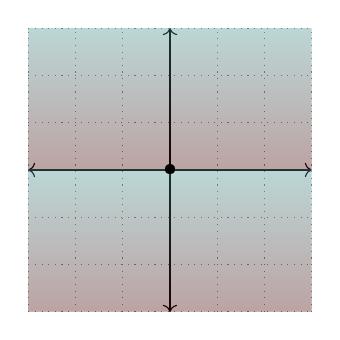
\begin{tikzpicture}[scale=0.6]
   	 \draw[dotted,step=1,gray,] (-3,-3) grid (3,3);
   	 \draw[->] (0,0) -- (0,3);
   	 \draw[->] (0,0) -- (0,-3);
   	 \draw[->] (0,0) -- (3,0);
   	 \draw[->] (0,0) -- (-3,0);
   	 	 \fill[bottom color=red!50!black, top color=cyan!50, opacity=0.2]
  (0,0) -- (3,0) -- (3,3) -- (0,3) -- (0,0);
   	 	 \fill[bottom color=red!50!black, top color=cyan!50, opacity=0.2]
  (0,0) -- (-3,0) -- (-3,3) -- (0,3) -- (0,0);
   	 	 \fill[bottom color=red!50!black, top color=cyan!50, opacity=0.2]
  (0,0) -- (3,0) -- (3,-3) -- (0,-3) -- (0,0);
    	 \fill[bottom color=red!50!black, top color=cyan!50, opacity=0.2]
  (0,0) -- (-3,0) -- (-3,-3) -- (0,-3) -- (0,0);
   	 \draw (0,0) node {\textbullet};
	\end{tikzpicture}
	\caption*{$\Sigma \subset N_\QQ$}
\end{figure}
\end{example}
We recall the combinatorial description of equivariant polarizations of toric varieties via convex polytopes. Suppose we have a complete fan \(\Sigma\), with rays \(\Sigma(1)\). Any Cartier divisor on \(X = \TV(\Sigma)\) is linearly equivalent to a \(T\)-equivariant one, and in summary we have the following exact sequence:
\[
0 \to M \to \cadiv_T(X) \cong \ZZ^{\Sigma(1)} \to \Cl(X) \to 0.
\]
and more explicitely we have the relations \(\div(\chi^u) = \sum_{\rho \in \Sigma(1)} \langle u, v_\rho \rangle D_\rho\).

Recall that to any lattice polytope \(P \subset M_\QQ\) we can associate a normal projective toric variety \(X_P\) given by its dual fan, and an ample divisor \(D_P\) given by coefficients on the ray generators of \(\Sigma(1)\) specified by the equations of halfspaces defining \(P\).
\begin{example}
If we start with \(P\) being the following polytope
\begin{figure}[h]
\centering
  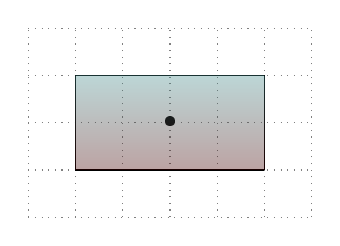
\begin{tikzpicture}[scale=0.6]
   	 \draw[dotted,step=1,gray,] (-3,-2) grid (3,2);
   	 \draw[] (2,-1) -- (2,1) -- (-2,1) -- (-2,-1) -- (2,-1);
   	 \draw (0,0) node {\textbullet};
   	 \fill[bottom color=red!50!black, top color=cyan!50, opacity=0.2]
  (2,-1) -- (2,1) -- (-2,1) -- (-2,-1) -- (2,-1);   	 
	\end{tikzpicture}
	\caption*{$P \subset M_\QQ$}
\end{figure}

Then the normal fan \(\mathcal{N}(P)\) is that of \(\PP^1 \times \PP^1\) as in example (ref). We can calculate the corresponding divisor as
\[
D_P = -2D_{e_1} - D_{e_2} -2 D_{-e_1} - D_{-e_2}  \sim -4 D_{e_1} -2 D_{e_2} 
\]
Where the coefficient at is given by () for example. We see that this divisor represents the line bundle \(\O(4,2)\). (check)
\end{example}
Moreover any equivariant polarization of a toric variety \((X,D)\) may be constructed from some polytope, via the exact sequence (ref).
\subsection{Complexity one $T$-varieties}
There is a successful program to extend the combinatorial dictionary of toric varieties to \(T\)-varieties of higher complexity. Roughly speaking, the combinatorial data lives over the Chow quotient of \(X\) by the \(T\)-action.

Recall that one may define an abelian semigroup structure on the set of all polyhedra via Minkowski addition:
\[
\Delta + \Delta' := \{ v + v' | v \in \Delta, \ v' \in \Delta' \}.
\]
It is well known that this gives a representation of any polyhedron \(\Delta = P + \sigma \) where \(P\) is a convex polytope and \(\sigma\). The cone \(\sigma\) is uniquely specified and is known as the tail cone of \(\Delta\). We will write \(\tail \Delta = \sigma\), and call \(\Delta\) a \(\sigma\)-tailed polyhedra in this situation.

The set of \(\sigma\)-tailed polyhedra form a sub-semigroup \(\Pol_\QQ^+(N,\sigma)\). We also include \(\emptyset\) here, with \(\emptyset + \Delta := \emptyset\) for any \(\Delta\). We may now recall the definition of a polyhedral divisor:
\begin{definition}
Let \(\sigma \subset N_\RR\) be a cone, and \(Y\) a normal projective variety over \(\CC\). A polyhedral divisor on \((Y,N)\) with tail cone \(\sigma\) is an element \(\mathcal{D} \in \Pol_\QQ^+(N,\sigma) \otimes \cadiv_\QQ^+(Y)\), where \(\cadiv_\QQ^+(Y)\) is the semigroup of effective \(\QQ\)-Cartier divisors on \(Y\). We write \(\tail \D = \sigma\).
\end{definition}
Let \(\Loc \D := Y \backslash \bigcup_{\D_Z = \emptyset} Z\). The evaluation of \(\D\) at \(u \in \sigma^\vee\) is defined to be the \(\QQ\)-Cartier divisor on \(Y\) given by:
\[
\D(u) :=  \sum_{\D \neq \emptyset} \min_{v \in \D_P} \langle v,u \rangle Z_{|\Loc \D}.
\]
\begin{definition}
A polyhedral divisor \(\D\), as defined above, is called a \(p\)-divisor if \(\D(u)\) is semiample for \(u \in \sigma^\vee\) and, in addition, big for \(u \in \text{int}(\sigma^\vee)\). Note if \(\Loc \D\) affine this is automatically satisfied.
\end{definition}

By \cite[Proposition 3.1]{hausen2018torus}, \(p\)-divisor defines an affine \(T\)-variety in the following manner. Note for \(u \in \sigma^\vee\) we have \(\D(u) + \D(u') \le \D(u+u')\). Consider the sheaf of \(N\)-graded algebras
\[
\mathcal{A} := \bigoplus_{w \in \sigma^{\vee}} \O_{\Loc \D} (\D(u)).
\]
Define \(\TV(\D) := \spec H^0(\Loc \D, \mathcal{A}) \). Note the semiample and big conditions in the definition of a \(p\)-divisor ensure that the algebra \(H^0(\Loc \D, \A)\) is finitely generated.

The resulting \(T\)-variety \(\TV(\D)\) remains unchanged if we pull back \(\D\) by some birational \(\varphi: Y' \to Y\), i.e if \(\D' := \) then \(\TV(\D') = \TV(\D)\). Moreover, modifying \(\D\) by an element in the image of the natural map
\[
N \otimes_\ZZ \CC(Y)^* \to \Pol_\QQ^+(N,\sigma) \otimes \cadiv_\QQ^+(Y)
\]
also does not change \(\TV(\D)\). Such an element is known as a \textit{principal polyhedral divisor}

In the converse direction, by \cite[Proposition 3.4]{hausen2018torus}, any affine \(T\)-variety \(X\) is of the form \(\TV(\D)\) for some \(p\)-divisor \(\D\). In fact one can define morphisms of \(p\)-divisors, and this correspondence turns out to be an equivlance of categories between affine \(T\)-varieties and \(p\)-divisors up to equivalence via the modifications mentioned above.
\begin{example}
downgrade situation, toric example,
\end{example}

In complexity one, \(Y\) is a curve. Here the degree polyhedron
\[
\deg \D :=
\]
plays an important role. Note the condition (ref) becomes X. Either \(\Loc \)... Therefore any complexity one normal affine \(\T\)-variety may be realized as \(\TV(\D)\) where \(\D\) is a \(p\)-divisor over \(\PP^1\).

By (ref) we have a method of gluing \(p\)-divisors in a natural way to construct general \(T\)-varieties, generalizing the notion of a fan of cones in the toric case. Here we recall the situation in complexity one, where this gluing data is simplified using degree polyhedra, 

By a \textit{complete polyhedral decomposition} we mean a decomposition of \(N_\QQ\) into a collection of polyhedra, closed under intersection. A complete polyhedral decomposition will have a \textit{tail fan}: a fan comprised of exactly the tail cones of the polyhedra in the decomposition. If \(\mathcal{G}\) is a polyhedral decomposition then we write \(\tail \mathcal{G}\) for its tail fan, and for \(\sigma \in \tail \mathcal{G}\) we write  \(\mathcal{G}^\sigma\) for the polyhedron in \(\mathcal{G}\) with tail cone \(\sigma\).

Minkowski addition of polyhedra lifts to the level of complete polyhedral decompositions with a prescribed tail fan. For a given fan \(\Sigma\) denote by \(\PD^+_\QQ(N,\Sigma)\) the corresponding semigroup.

\begin{definition}
A complete \(f\)-divisor is a pair \(\mathcal{S} = \left( \sum_{y \in \PP^1} S_y \otimes \{y\}, \ \deg \mathcal{S} \right)\) where
\[
\sum_{y \in \PP^1} S_y \otimes \{y\} \in \PD^+_\QQ(N,\Sigma) \otimes \cadiv_+(\PP^1)
\] such that for any \(\sigma \in \Sigma\) either \(\sigma \cap \deg \mathcal{S} = \emptyset \) or the polyhedral divisor \(S^\sigma := \sum S_y^\sigma \otimes \{y\}\) is a \(p\)-divisor. We call the finite collection of \(S_y \neq \Sigma\) the non-trivial slices of \(S\).
\end{definition}
\begin{example}
Here we give an example of an \(f\)-divisor describing a complexity one threefold. 
\begin{figure}[h]
\centering


\label{fig:fdivex}
\resizebox{0.9\linewidth}{!}{
\begin{subfigure}[b]{0.30\textwidth}
\centering
  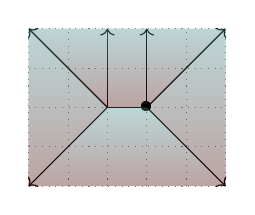
\begin{tikzpicture}[scale=0.5]
   	 \draw[dotted,step=1,gray,] (-3,-2) grid (2,2);
   	 \draw[->] (0,0) -- (0,2);
   	 \draw[] (0,0) -- (-1,0);
   	 \draw[->] (-1,0) -- (-1,2);
   	 \draw[->] (0,0) -- (2,2);
   	 \draw[->] (0,0) -- (2,-2);
   	 \draw[->] (-1,0) -- (-3,2);
   	 \draw[->] (-1,0) -- (-3,-2);
   	 \fill[bottom color=red!50!black, top color=cyan!50, opacity=0.2]
  (0,0) -- (2,-2) -- (2,2) -- (0,0);
   	 \fill[bottom color=red!50!black, top color=cyan!50, opacity=0.2]
  (0,0) -- (2,2) -- (0,2) -- (0,0);
   	 \fill[bottom color=red!50!black, top color=cyan!50, opacity=0.2]
  (0,0) -- (0,2) -- (-1,2) -- (-1,0) -- (0,0);
	 \fill[bottom color=red!50!black, top color=cyan!50, opacity=0.2]
  (-1,0) -- (-1,2) -- (-3,2) -- (-1,0);
  	 \fill[bottom color=red!50!black, top color=cyan!50, opacity=0.2]
  (-1,0) -- (-3,2) -- (-3,-2) -- (-1,0);
   	 \draw (0,0) node {\textbullet};
	 \fill[bottom color=red!50!black, top color=cyan!50, opacity=0.2]
  (0,0) -- (-1,0) -- (-3,-2) -- (2,-2) -- (0,0);
	\end{tikzpicture}
	\caption*{$\mathcal{S}_0$}
\end{subfigure}
\begin{subfigure}[b]{0.30\textwidth}
	\centering
  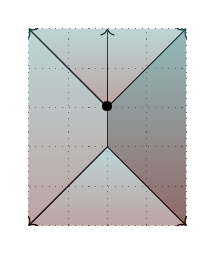
\begin{tikzpicture}[scale=0.5]
   	 \draw[dotted,step=1,gray,] (-2,-3) grid (2,2);
   	 \draw[->] (0,0) -- (0,2);
   	 \draw[] (0,0) -- (0,-1);
   	 \draw[->] (0,0) -- (2,2);
   	 \draw[->] (0,0) -- (-2,2);
   	 \draw[->] (0,-1) -- (2,-3);
   	 \draw[->] (0,-1) -- (-2,-3);
	 \fill[bottom color=red!50!black, top color=cyan!50, opacity=0.2]
  (0,0) -- (0,-1) -- (2,-3) -- (2,2) -- (0,0);
	 \fill[bottom color=red!50!black, top color=cyan!50, opacity=0.2]
  (0,0) -- (2,2) -- (0,2) -- (0,0);
	 \fill[bottom color=red!50!black, top color=cyan!50, opacity=0.2]
  (0,0) -- (0,2) -- (-2,2) -- (0,0);
  	 \fill[bottom color=red!50!black, top color=cyan!50, opacity=0.2]
  (0,0) -- (0,-1) -- (2,-3) -- (2,2) -- (0,0);
  	 \fill[bottom color=red!50!black, top color=cyan!50, opacity=0.2]
  (0,0) -- (-2,2) -- (-2,-3) -- (0,-1) -- (0,0);
  	 \fill[bottom color=red!50!black, top color=cyan!50, opacity=0.2]
  (0,-1) -- (2,-3) -- (-2,-3) -- (0,-1);
   	 \draw (0,0) node {\textbullet};
	\end{tikzpicture}
	\caption*{$\mathcal{S}_1$}
\end{subfigure}
\begin{subfigure}[b]{0.30\textwidth}
	\centering
  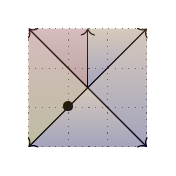
\begin{tikzpicture}[scale=0.5]
   	 \draw[dotted,step=1,gray,] (-1,-1) grid (2,2);
   	 \draw[->] (0.5,0.5) -- (2,2);
   	 \draw[->] (0.5,0.5) -- (0.5,2);
   	 \draw[->] (0.5,0.5) -- (-1,2);
   	 \draw[->] (0.5,0.5) -- (-1,-1);
   	 \draw[->] (0.5,0.5) -- (2,-1);
   	 \draw (0,0) node {\textbullet};
   	           \fill[bottom color=blue!50!black, top color=orange!50, opacity=0.2]
  (0.5,0.5) -- (2,2) -- (2,-1) -- (0.5,0.5);
   	           \fill[bottom color=yellow!50!black, top color=red!50, opacity=0.2]
  (0.5,0.5) -- (-1,2) -- (-1,-1) -- (0.5,0.5);
   	           \fill[bottom color=blue!50!black, top color=orange!50, opacity=0.2]
  (0.5,0.5) -- (2,2) -- (0.5,2) -- (0.5,0.5);
   	           \fill[bottom color=red!50!black, top color=red!50, opacity=0.2]
  (0.5,0.5) -- (-1,2) -- (0.5,2) -- (0.5,0.5);
   	           \fill[bottom color=blue!50!black, top color=orange!50, opacity=0.2]
  (0.5,0.5) -- (2,-1) -- (-1,-1) -- (0.5,0.5);
  
	\end{tikzpicture}
	\caption*{$\mathcal{S}_{\infty}$}
\end{subfigure}
\begin{subfigure}[b]{0.40\textwidth}
	\centering
  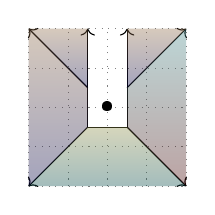
\begin{tikzpicture}[scale=0.5]
   	 \draw[dotted,step=1,gray,] (-2,-2) grid (2,2);
   	 \draw[] (-0.5,-0.5) -- (0.5,-0.5);
   	 \draw[->] (-0.5,-0.5) -- (-0.5,2);
   	 \draw[->] (0.5,-0.5) -- (0.5,2);
   	 \draw[->] (0.5,0.5) -- (2,2);
   	 \draw[->] (-0.5,0.5) -- (-2,2);
   	 \draw[->] (-0.5,-0.5) -- (-2,-2);
  	 \draw[->] (0.5,-0.5) -- (2,-2);
   	 \draw (0,0) node {\textbullet};
   	 \fill[bottom color=red!50!black, top color=cyan!50, opacity=0.2]
  (2,-2) -- (0.5,-0.5) -- (0.5,0.5) -- (2,2) -- (2,-2);
      \fill[bottom color=cyan!50!black, top color=yellow!50, opacity=0.2]
  (2,-2) -- (0.5,-0.5) -- (-0.5,-0.5) -- (-2,-2) -- (2,-2);
      \fill[bottom color=blue!50!black, top color=orange!50, opacity=0.2]
  (-2,-2) -- (-0.5,-0.5) -- (-0.5,0.5) -- (-2,2) -- (-2,-2);
        \fill[bottom color=blue!50!black, top color=orange!50, opacity=0.2]
  (0.5,0.5) -- (0.5,2) -- (2,2) -- (0.5,0.5);
          \fill[bottom color=blue!50!black, top color=orange!50, opacity=0.2]
  (-0.5,0.5) -- (-0.5,2) -- (-2,2) -- (-0.5,0.5);
	\end{tikzpicture}
	\caption*{$\deg \mathcal{S}$}
\end{subfigure}
}
\end{figure}
\end{example}

In complexity one there is a generalization of the correspondence between lattice polytopes and polarized projective toric varieties. We recall the definition of a divisorial polytope, which is used to generalize the polytope description of a polarized toric variety to the complexity one case.
\begin{definition}
A divisorial polytope is a function \(\Psi\) on a lattice polytope \(\Box \subset M_\RR\):
\[
\Psi: \Box \to \wdiv_\RR \PP^1, \ u \mapsto \Sigma_{y \in \PP^1} \Psi_y(u) \cdot \{y\},
\]
such that:
\begin{itemize}
\item For \(y \in \PP^1\) the function \(\Psi_y: \Box \to \RR\) is the minimum of finitely many  affine functions, and \(\Psi_y \equiv 0\) for all but finitely many \(y \in \PP^1\).
\item Each \(\Psi_y\) takes integral values at the vertices of the polyhedral decomposition its regions of affine linearity induce on \(\Box\).
\item \(\deg \Psi(u) > -2\) for \(u \in \text{int} (\Box)\);
\end{itemize}
A divisorial polytope is said to be Fano if additionally we have that:
\begin{itemize}
\item The origin is an interior lattice point of \(\Box\).
\item The affine linear pieces of each  \(\Psi_y\) are of the form \(u \mapsto \frac{\langle v,u \rangle - \beta + 1}{\beta}\) for some primitive lattice element \(v \in N\);
\item Every facet \(F\) of \(\Box\) with \((\deg \circ \Psi _{|F}) \neq -2\) has lattice distance \(1\) from the origin.
\end{itemize}
\end{definition}
Let \(\Psi\) be a divisorial polytope. We may construct a complexity one polarized \(T\)-variety from the graded ring \(S\) given by: 
\[
S_k := \bigoplus_{u \in \Box \cap \frac{1}{k} M} H^0(\PP^1, \mathcal{O}(\lfloor k \cdot ( \Psi(u) +D) \rfloor),
\]
where \(D\) is some integral divisor of degree \(2\). We may also recover a divisorial polytope \(\Psi\) from any polarized complexity one \(T\)-variety \((X,L)\) such that \( H^0(X,L^k) = S_k\). Moreover Fano divisorial polytopes correspond to Fano \(T\)-varieties \((X,-K_X)\). Thus all Fano complexity one \(T\)-varieties may be described in this way. For more details of this construction and the correspondence see \cite{suss2013fano}.

We now recall some basic terminology for divisorial polytopes, which we will make use of in later sections. The push-forward of the measure induced by \(\omega\) is known as the Duistermaat-Heckman measure, independent of the choice of \(\omega\) and which we denote by \(\nu\). Denote the standard measure on \(M_\RR\) by \(\eta\).

\begin{definition}
Let \(\Psi\) be a divisorial polytope.
\begin{itemize}
\item The degree of \(\Psi\) is the map \( \deg \Psi : \Box \to \RR\) given by \( u \mapsto \deg (\Psi(u))\).
\item The barycenter of \(\Psi\) is \(\bc(\Psi) \in \Box\), such that for all \(v \in N_\RR\):
\[
\langle \bc(\Psi), v \rangle = \int_\Box v \cdot \deg \Psi \ d \eta = \int_\Box v d \nu. 
\]
Note by the second equality we see \(\bc(\Psi) = \bc_\nu(\Box).\)
\item The volume of \(\Psi\) is defined to be:
\[
\vol \Psi = \int_\Box \deg \Psi \ d \eta = \int_\Box d \nu.
\]
\end{itemize}
\end{definition}

A Fano divisorial polytope fixes a distinguished representative of \(-K_X\) and specifies a linearisation of the action of \(T\) to \((X,-K_X)\). By the proof of \cite[Theorem 3.21]{petersen2011torus} it is seen that the linearisation coincides with the canonical linearisation of \((X,-K_X)\), and so the moment map specified by the divisorial polytope, with image \(\Box\), coincides with the moment specified by the canonical linearisation.

From here on let \((X,-K_X)\) be the polarized complexity one Fano \(T\)-manifold given by a fixed divisorial polytope \(\Psi: \Box \to \wdiv_\RR \PP^1\), with \(\bc_\nu(\Box) \neq 0\).

\section{Equivariant $K$-stability}
In this section we recall definitions of \(K\)-stability. In summary the \(K\)-stability criteria are concerned with the positivity of certain numerical invariants associated to \textit{test configurations} of our original space. We do not go into detail about how or why \(K\)-stability should relate to the existence of canonical metrics here, but give the definitions and theorems we will rely on later in the thesis.
\subsection{Twisted equivariant $K$-stability}
\label{prelim:twisted}
Here we recall notions of Twisted equivariant $K$-stability, following \cite{datar2016kahler}. Let \(X\) be a Fano manifold with the action of a complex reductive group \(G\) of automorphisms containing a maximal torus \(T\). Fix a \(T\)-invariant K\"ahler form \(\omega \in 2 \pi c_1(X)\) induced by the Fano condition. Recall that the Lie algebra \(\mathfrak{t}\) of the maximal compact torus in \(T\) may be identified with \(N_\RR = N \otimes \RR\).
\begin{definition}
A \(G\)-equivariant test configuration for \((X,L)\) is a \(\CC^*\)-equivariant flat family \(\X\) over the affine line equipped with a relatively ample equivariant \(\QQ\)-line bundle \(\mathcal{L}\) such that:
\begin{enumerate}
\item The \(\CC^*\)-action \(\lambda\) on \((\X, \mathcal{L})\) lifts the standard action on \(\mathbb{A}^1\);
\item The general fiber is isomorphic to \(X\) and \(\mathcal{L}\) is the relative anti-canonical bundle of \(\X \to \mathbb{A}^1\).
\item The action of \(G\) extends to \((\X,\mathcal{L})\) and commutes with the \(\CC^*\)-action \(\lambda\).
\end{enumerate}
A test configuration with \(\X \cong X \times \mathbb{A}^1\) is called a product configuration. If such an isomorphism exists and is \(\CC^*\)-equivariant then we call the test configuration trivial. Finally a test configuration with normal special fiber is called special.
\end{definition}
We work with \(G = T\) being a maximal torus in \(\Aut(X)\). We then have an induced \(T' = T \times \CC^*\)-action on the special fiber. The canonical lift of \(T'\)-action to \(-K_{\X_0}\) induces a canonical choice of moment map \(\mu: \X_0 \to M_\RR'\). The restriction of \(\lambda\) to \(\X_0\) is generated by the imaginary part of a \(T'\)-invariant vector field \(w\), and by an abuse of notation we also write \(w \in N'_\RR\) for the corresponding  one-parameter subgroup. The moment map \(\mu\) then specifies Hamiltonian functions \(\theta_w := \langle \mu, w \rangle: \X_0 \to \RR  \), as we have seen in Section~\ref{basics:momentmaps}.


\begin{definition}
The twisted Donaldson-Futaki character of a special test configuration \((\X, \mathcal{L}) \) is given by:
\[
\DF_{t,\xi}(\X,\mathcal{L},w) = \DF_{\xi}(\X,\mathcal{L},w) + \frac{(1-t)}{V} \int_{\X_0} ( \max_{\X_0} \theta_w - \theta_w)e^{\theta_\xi} \ \omega^n . 
\]
where \(V = \frac{1}{n!} \int_{\X_0} \omega^n\) is the volume of \(\X_0\), and \(\DF_\xi(\X,\L,w) = \frac{1}{V} \int_{\X_0} \theta_w \omega^n\) is the modified Donaldson-Futaki invariant of the configuration, in the form given in \cite[Lemma 3.4]{berman2014complex}.
\end{definition}
\begin{definition}
We say the triple  \((X,t,\xi)\) is \(G\)-equivariantly \(K\)-semistable if \( \DF_{t,\xi}(\X,\mathcal{L},w) \ge 0\) for all \(G\)-equivariant special configurations \((\X,\mathcal{L},w)\). We say \((X,t,\xi)\) is \(K\)-stable if in addition equality holds precisely for product configurations. 
\end{definition}
We will use the following theorem later:
\begin{theorem}[Berman-Witt-Nystrom] \label{thm:BWN}
If \((X,\xi)\) admits a K\"ahler-Ricci soliton then \((X,\xi)\) is \(K\)-stable.
\end{theorem}
From (Datar and Sze) we have a result in the converse direction:
\begin{theorem}[{\cite[Proposition 10]{datar2016kahler}} ] \label{thm:DS}
Let \(X\) be a polarized Fano manifold, with K\"ahler form \(\omega\). Let \(t \in [0,1]\) and \(\xi\) be a soliton candidate for \(X\). Then \((X,t)\) is \(G\)-equivariantly \(K\)-semistable only if for all \(s <t\)  there exists \(\omega_s \in 2 \pi c_1(X)\) such that \(\Ric(\omega_s) - \mathcal{L}_\xi \omega_s = s \omega_s + (1-s) \omega\).
\end{theorem}
\subsection{$K$-stability of $T$-varieties} \label{subsec:IS}
Here we review \(K\)-stability in complexity one. In \cite{ilten2015} Ilten and Suess described non-product special test configurations for a \(T\)-variety of complexity one in terms of its divisorial polytope. We first recall, from \cite{ilten2015}, the description of special fibers of non-product special configurations.

Let \(X\) be a Fano \(T\)-variety of complexity \(1\), corresponding to the Fano divisorial polytope \(\Psi : \Box \to Y\). Without loss of generality we may assume \(Y = \PP^1\). Then there exists some \(y \in \PP^1\), with at most one of \(\Psi_z\) having non-integral slope at any \(u \in \Box\) for \(z \neq y\), such that \(\X_0\) is the toric variety corresponding to the following polytope:
\begin{equation*}
\Delta_y := \Big\{(u,r) \in M_\RR \times \RR \; \Big| \; u \in \Box,\; -1-\sum_{z \neq y} \Psi_z(u) \leq r \leq 1+\Psi_y(u)\Big\}.\label{eq:special-fibre}
\end{equation*}

Furthermore, the induced \(\CC^*\)-action on \(\X_0\) is given by the one-parameter subgroup of 
 \(T' = T \times \CC^*\) corresponding to \(v'=(-mv,m) \in N \times \ZZ\), for some \(v \in N\). In fact it turns out, from \cite{ilten2015}, it is enough to consider those configurations with \(m=1\). As observed in \cite{ilten2015}, we obtain a description of the (non-twisted) Donaldson-Futaki character of $(\X_0,\xi')$:
\begin{equation}
\DF_{\X_0, \xi'}(v') = \frac{1}{\vol \Delta_y}\left(\int_{\Delta_y} \langle u', v' \rangle \cdot e^{\langle u', \xi'\rangle} du'\right),\label{eq:futaki-character}
\end{equation}
with $\xi',v' \in N_\RR \times \RR$. On the other hand, for $v,\xi \in N_\RR$ one obtains:
\begin{equation}
\DF_{X, \xi}(v) = F_{\X_0, (\xi,0)}((v,0))
= \frac{1}{\int_\Box \deg \bar \Phi(u) \,du }\left(\int_{\Box} \langle u, v \rangle \cdot \deg \bar \Phi(u) \cdot e^{\langle u, \xi \rangle}\, du\right)
, \label{eq:futaki-general-fibre}
\end{equation}

%\chapter{K\"ahler-Ricci solitons on Fano threefolds} \label{chap:sol}

\chaptermark{K\"ahler-Ricci solitons on Fano threefolds}


In this chapter we prove the following theorem:
\begin{theorem}[{\cite[Theorem 1.8]{cable2018classification}}] \label{thm:sol}
The Fano threefolds \(2.30, \ 2.31, \ 3.18, \ 3.22, \ 3.23, \ 3.24, \ 4.8\) from Mori and Mukai's classification \cite{mori1981classification} admit a non-trivial K\"ahler-Ricci soliton.
\end{theorem}
Together with \cite[Theorems. 6.1, 6.2]{ilten2015} it follows that all known smooth Fano threefolds with an effective complexity-one torus action admit a K\"ahler-Ricci soliton. We follow the joint work of \cite{cable2018classification}. We describe here the contribution of the author of this thesis to this article, namely to perform calculations to test the \(K\)-stability of threefolds and thus determine which admitted K\"ahler-Ricci solitons.

\section{The method of proof}
This proof of Theorem~\ref{thm:sol} is somewhat calculational in nature, and uses some computer assistance. We provide some context to our approach. At the end of this subsection we provide a more formal proof.

Let \(X\) be a smooth complexity one Fano \(T\)-variety. Recall the definition of a K\"ahler-Ricci soliton from definition \ref{def:tKRS}. We test for the existence of a K\"ahler-Ricci soliton on \(X\) using Theorem~\ref{thm:DS}. Recall from section~\ref{sec:toric} that the polarization \((X,-K_X)\) corresponds to a Fano divisorial polytope \(\Phi: \Box \to \Div \PP^1\), as defined in \ref{def:divpol}.

First we use Theorem \ref{thm:BWN} to find candidate vector fields \(\xi \in N_\RR\) for a soliton. By Theorem~\ref{thm:BWN}, any such \(\xi\) will satisfy the following equation: 
\begin{equation} \label{eq:producteq}
\DF_{\xi}(X \times \mathbb{A}^1, w) = 0.
\end{equation}
For all \(w \in N'_\RR\). By \ref{eq:futaki-character} this becomes:
\begin{equation} \label{eq:combproducteq}
\int_{\Box} \langle u, v \rangle \cdot \deg \bar \Phi(u) \cdot e^{\langle u, \xi \rangle}\, du = 0
\end{equation}
By the arguments in \cite[Section~3.1]{donaldson2008kahler} there always exist a unique choice $\xi \in N_\RR$ for which this holds. We refer to such a $\xi$ as a \textit{soliton canditate}.

The integral (\ref{eq:combproducteq}) may be solved symbolically, outputting an exponential polynomial \(g(\xi, e^{\xi})\) in \(\xi\). In practice however, the domain \(P\) can complicate the calculation for \(\dim X > 2\). To deal with this we developed a recursive algorithm, based on results of Barvinok \cite{Barvinok1992}, which reduces the integral to evaluations at the vertices of \(P\). We explain this algorithm at the end of this chapter.

For our examples the equation \(g(\xi,e^{\xi}) = 0\) is impossible to solve analytically. To get around this we use \textit{real interval arithmetic} (RIA) estimates to find some hypercube \(D\) in which the solution \(\xi\) lies. For each special test configuration \((\X,w)\) we then use further RIA to show that \(\DF_{\xi'}(\X,W)>0\) For \(\xi \in D\). In Table~\ref{table:solitontable} below we give estimates found for the vector field \(\xi\) for each threefold in the list of \cite{suss2013fano}. The threefolds 3.8*, 3.21, 4.5 were shown to admit a non-trivial K\"ahler-Ricci soliton in \cite{ilten2015}. We can show that our approximations are correct to the nearest \(10^{-5}\).

When \(\dim  X = 2\) the process of finding suitable \(D\) via RIA is a simple application of the intermediate value theorem. For \(\dim X >2 \) we cannot immediately use the intermediate value theorem to obtain \(D\). In all but one of our examples we make use of additional symmetries to reduce to a one-dimensional problem. Given an automorphism \(\sigma \in \GL(M)\) permuting the vertices of \(\Box\) such that \(\deg (\Phi \circ \sigma) = \deg \Phi\), by (\ref{eq:futaki-general-fibre}) we have:
\[
\DF_{X, \sigma^{\!*}\!(\xi)}  =  \DF_{X, \xi} \ \circ \ \sigma^*
\]

Since \(\xi \in N_\mathbb{R}\) is the unique solution to \(F_{X,\xi} = 0\), this gives \(\xi \in N_{\mathbb{R}}^{\sigma^*}\). For \(\dim X = 3\) we have \(\dim N_{\mathbb{R}}^{\sigma^*}  = 1\) and we are in a situation where intermediate value theorem may be used to find \(D\). Note that in threefold 3.23 there is no such involution, and we must take another approach, which we explain in the proof below and in Example~\ref{ex:assym}.
%
%
%
\begin{table}[H]  \centering
\captionsetup{width=.95\linewidth}
\caption{Fano threefolds and their soliton vector fields in the canonical coordinates coming with the representation of the combinatorial data in \cite{suss2013fano}.}  \label{table:solitontable}
\begin{tabular}{l l l}
\toprule
Threefold & $\xi$ & \\ \hline
Q & $(0,0)$ \\
2.24* & $(0,0)$ \\
2.29 & $(0,0)$ \\
2.30 & $(0,0.51489)$ \\
2.31 & $(0.28550,0.28550)$\\
2.32 & $(0,0)$ \\
3.8* & $(0,-0.76905)$ \\
3.10* & $(0,0)$ \\
3.18 & $(0,0.37970)$ \\
3.19 & $(0,0)$ \\
3.20 & $(0,0)$ \\
3.21 & $(-0.69622,-0.69622)$ \\
3.22 & $(0,0.91479)$ \\
3.23 & $(0.26618,  0.67164)$ \\
3.24 & $(0,0.43475)$ \\
4.4 &  $(0,0)$ \\
4.5* &  $(-0.31043,-0.31043)$ \\
4.7 &  $(0,0)$ \\
4.8 &  $(0,0.62431)$ \\
\bottomrule
\end{tabular}
\label{table:name}
\end{table}
We now give a more formal proof of Theorem~\ref{thm:sol}. The complete calculations for the proof are performed using SageMath, and can be found as an online worksheet\footnote{CoCalc:\url{https://cocalc.com/projects/ae8e1663-e2ad-40b8-aec2-30faf4e6a54f/files/threefolds.sagews}}.
\begin{proof}[Proof of Theorem~\ref{thm:sol}]
Note the data required for this proof is collated in Appendix~\ref{appendix1}. The divisorial polytopes were originally given in \cite{suss2013fano}, although the piecewise affine \(\Psi\) discussed there differs from our divisorial polytope \(\Phi\) by the divisor \(D = 2 \cdot \{ \infty \}\).

In threefolds 2.31, 3.18, 3.22, 3.24 and 4.8 there exists a non-trivial involution \(\sigma \in \GL(M)\) permuting the vertices of \(\Box\), such that \(\deg (\Phi \circ \sigma) = \deg \Phi\). Choose a basis $e_1, e_2$ of $N_\RR$ with $\sigma^*(e_1)=-e_1$ and $\sigma^*(e_2)=e_2$. The soliton candidate $\xi = (\xi_1,\xi_2)$ must be contained in the line $N_\RR^{\sigma^*} = \RR e_2$. For each of these example we obtain an interval \(D\) where the soliton candidate must lie, via the intermediate value theorem and RIA, see Appendix~\ref{appendix1}.

Recall the description of non-product special test configuration spaces from \ref{subsec:IS}. In Appendix~\ref{appendix1} we provide closed forms for \(h_y(\xi_2) := (\vol \Delta_y) \cdot \DF_{\xi_2 e_2}(\X,(0,1))\) for every admissible choice of $y \in \PP^1$, using the algorithm described in \ref{sec:barvinok}. We also provide lower bounds on \(h_y(D)\) using further RIA, ensuring the positivity of $\DF_{\xi_2 e_2}(\X_{y,0,1})$. These threefolds then admit a K\"ahler-Ricci soliton by Theorem~\ref{thm:DS}. See Example~\ref{ex:sym} for details of the computation and Appendix~\ref{appendix2} for the implementation in SageMath.

For the case of threefold no. 3.23 there is no involution fixing $\deg \Phi$. In this case we take a more general approach to bound the value of the candidate \(\xi\). Here we make use of some elementary calculus. Note, that \(\xi\) is the unique solution to the equation \(\nabla_n G = 0 \), where 
\[
G(v) := \int_{\Box} \deg \bar \Phi(u) \cdot e^{\langle u, v \rangle}\, du = 
\int_{\Delta_0} e^{\langle u', (v,0) \rangle} \, du'.
\]
We identify a rectangular region \(D \subset \RR^2 \) such that \(\nabla_n G > 0 \) holds along \(\partial D\), where \(n\) is any unit outer normal of the rectangle \(D\). Since $D$ is compact it must contain a local minimum of $G$, which then cannot lie on \(\partial D\). We then have \(\xi\) in the interior of \(D\) such that \(\nabla_n G = 0\).

To show $\nabla_n G >0 $ along $\partial D$ we have to again use interval arithmetic. We determine a closed form which coincides with $\nabla_n G = \DF_\xi$ up to a positive constant. We subdivide the faces of the boundary into sufficiently small segments. Using RIA on the closed form for $\nabla_n G(\xi)$ we obtain the positivity result. See Example~\ref{ex:assym} for details of the computation and Appendix~\ref{appendix2} for the implementation in SageMath.
\end{proof}
\section{Two examples in detail}
Here we present threefolds 2.30 and 3.23 in detail:
\begin{example}[2.30 -- Blow up of quadric threefold in a point]
\label{exp:threefold}
Consider the threefold 2.30. The function \(\Phi\) is given in Figure~\ref{fig:data230}.
\begin{figure}[h]
\caption{The combinatorial data for threefold 2.30}
\label{fig:data230}
\resizebox{0.90\linewidth}{!}{
\begin{subfigure}[b]{0.30\textwidth}
\centering
  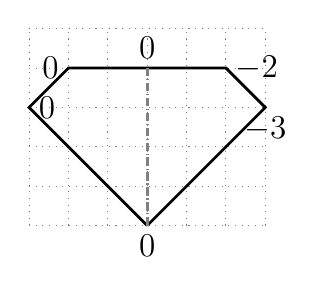
\begin{tikzpicture}[scale=0.5]
   	 \draw[dotted,step=1,gray,] (-3,-3) grid (3,2); \draw[line width = 1pt] (0,-3) --
     (-3,0) -- (-2,1)--(2,1)--
 	 (3,0)--(0,-3); \draw[densely dashdotted, gray, line width = 1.2pt] (0,-3) -- (0,1);
 	 \node at (0,-3) [below] {\large{$0$}};
 	 \node at (-3,0) [right] {\large{$0$}};
 	 \node at (-2,1) [left] {\large{$0$}};
 	 \node at (2,1) [right] {\large{$-2$}};
 	 \node at (3,0) [below] {\large{$-3$}};
 	 \node at (0,1) [above] {\large{$0$}};
	\end{tikzpicture}
	\caption*{$\Phi_0$}
\end{subfigure}
\begin{subfigure}[b]{0.30\textwidth}
	\centering
 	 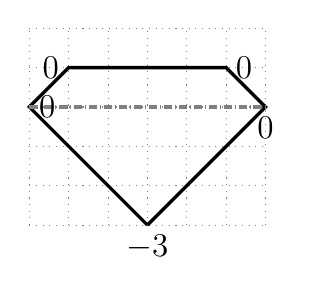
\begin{tikzpicture}[scale=0.5]
 	   \draw[dotted,step=1,gray] (-3,-3) grid (3,2); \draw[line width = 1.2pt] (0,-3) --
 	   (-3,0) -- (-2,1)--(2,1)--
 	   (3,0)--(0,-3); \draw[densely dashdotted, gray,line width = 1.2pt] (-3,0) -- (3,0);
 	 \node at (0,-3) [below] {\large{$-3$}};
 	 \node at (-3,0) [right] {\large{$0$}};
 	 \node at (-2,1) [left] {\large{$0$}};
 	 \node at (2,1) [right] {\large{$0$}};
 	 \node at (3,0) [below] {\large{$0$}};
	\end{tikzpicture}
	\caption*{$\Phi_1$}
\end{subfigure}
\begin{subfigure}[b]{0.30\textwidth}
	\centering
 	 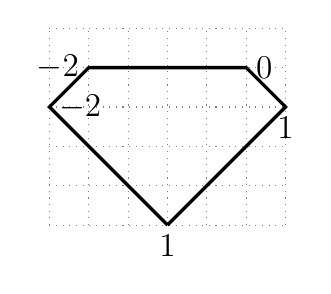
\begin{tikzpicture}[scale=0.5]
 	   \draw[dotted,step=1,gray] (-3,-3) grid (3,2); \draw[line width = 1.2pt] (0,-3) --
 	   (-3,0) -- (-2,1)--(2,1)--
 	   (3,0)--(0,-3);
 	 \node at (0,-3) [below] {\large{$1$}};
 	 \node at (-3,0) [right] {\large{$-2$}};
 	 \node at (-2,1) [left] {\large{$-2$}};
 	 \node at (2,1) [right] {\large{$0$}};
 	 \node at (3,0) [below] {\large{$1$}};
	\end{tikzpicture}
	\caption*{$\Phi_\infty$}
\end{subfigure}
\begin{subfigure}[b]{0.40\textwidth}
	\centering
 	 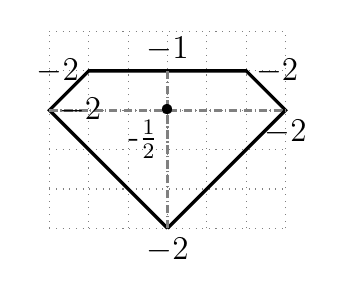
\begin{tikzpicture}[scale=0.5]
 	   \draw[dotted,step=1,gray] (-3,-3) grid (3,2); \draw[line width = 1.2pt] (0,-3) --
 	   (-3,0) -- (-2,1)--(2,1)--
 	   (3,0)--(0,-3); \draw[densely dashdotted, gray,line width = 1.2pt] (-3,0) -- (3,0); \draw[densely dashdotted, gray,line width = 1.2pt] (0,-3) -- (0,1) ;
 	 \node at (0,-3) [below] {\large{$-2$}};
 	 \node at (-3,0) [right] {\large{$-2$}};
 	 \node at (-2,1) [left] {\large{$-2$}};
 	 \node at (2,1) [right] {\large{$-2$}};
 	 \node at (3,0) [below] {\large{$-2$}};
 	 \node at (0,0) [below left] {\large{-$\frac{1}{2}$}};
 	 \node at (0,1) [above] {\large{$-1$}};
 	 \draw (0,0) node {\textbullet};
	\end{tikzpicture}
	\caption*{$\deg \Phi $}
\end{subfigure}
}
\end{figure}
We now find the unique candidate vector field \(\xi \in N_\mathbb{R}\) for a \(K\)-stable pair \((X,\xi)\). We see that $\deg \Phi$ is symmetric with respect to reflection $\sigma$ along the vertical axis. Hence, we have  \(\xi = \xi_2e_2\) for some \(\xi_2 \in \mathbb{R}\) and must find a solution $\xi_2$ to $F_{X,\xi_2e_2}=0$, which is equivalent to $F_{X,\xi_2e_2}(e_2)=0$. Indeed, we have 
\[F_{X,\xi_2e_2}(e_1) = F_{X,\sigma^*\xi_2e_2}(\sigma^*e_1)= F_{X,\xi_2e_2}(-e_1)= -F_{X,\xi_2e_2}(e_1).\]
Hence, $F_{X,\xi_2e_2}(e_1)=0$ and the claim follows by linearity.

By (\ref{eq:futaki-character}) the vanishing of $F_{X,\xi_2e_2}(e_2)$ is equivalent to that of
\[0=g(\xi_2) := \int_{\Box} u_2 \cdot \deg \bar \Phi(u) \cdot e^{u_2 \xi_2}\, du = \int_{\Delta_0} u_2 \cdot e^{u_2 \xi_2}\, du.\] Where the integral on the right hand side can be solved analytically. We obtain
\[
\frac{1}{\xi_{2}^{4}}\cdot\left({\left(2 \, \xi_{2}^{3} - 3 \, \xi_{2} - 3\right)} e^{\left(4 \, \xi_{2}\right)} + 12 \, \xi_{2} e^{\left(3 \, \xi_{2}\right)} + 3 \, \xi_{2} + 3\right) e^{\left(-3 \, \xi_{2}\right)}.
\]
Evaluating the exponential functions with a precision of 16 binary digits  and using elementary estimations it can be shown that \(g(0.514) <0\) and \(g(0.515)>0\). By the intermediate value theorem then \(0.514 < \xi_2 < 0.515\). It remains to check the positivity of the Donaldson-Futaki invariant for each degeneration. The degenerations of this threefold correspond to the polytopes:{
\begin{align*}
\Delta_0 &= \conv((-3,0,1),(-2,1,1),(2,1,-1),(3,0,-2),(0,-3,1),(0,1,1)); \\
\Delta_1 &= \conv((-3,0,1),(-2,1,1),(0,1,0),(2,1,1),(3,0,1),(0,-3,-2)); \\ 
\Delta_\infty &= \conv((-3,0,-1),(-2,1,-1),(2,1,1),(3,0,2),(0,-3,2),(0,0,-1),(0,1,-1)); \\
\Delta_y &= \conv((0, 0, -1/2), (3, 0, 1), (2, 1, 1), (0, 1, 0), (-2, 1, 1), (-3, 0, 1), (0, -3, 1)) \\ 
& \ \ \ ( \text{for } y 
\not \in \{0,1,\infty\} ).
\end{align*}}
In each case we have induced \(\CC^*\)-action given by \((0,0,1) \in N \times \ZZ \). Denote
\[
h_y(\xi_2) := (\vol \Delta_y) \cdot \DF_{(0,\xi_2)}(\X_{y,0,1}).
\]
Clearly positivity of \(h_y\) implies the positivity of \(\DF_\xi(\X_{y,0,1})\). 
Once more solving the integrals appearing in (\ref{eq:futaki-character}) analytically with $y \not \in \{0,1,\infty\}$  we obtain:
\begin{align*}
h_0(\xi_2) &= \frac{1}{3\xi_2^{4}}\cdot
{\left({\left(2   \xi_2^{3} - 3   \xi_2 - 3\right)} e^{4   \xi_2} + 3   {\left(3   \xi_2^{2} + 2\right)} e^{3   \xi_2} - 3   \xi_2 - 3\right)} e^{-3   \xi_2}
\\
h_1(\xi_2) &= \frac{1}{6   \xi_2^{4}}\cdot
{\left({\left(8   \xi_2^{3} + 6   \xi_2^{2} - 3\right)} e^{4   \xi_2} - 12   {\left(3   \xi_2^{2} - 3   \xi_2 + 1\right)} e^{3   \xi_2} + 12   \xi_2 + 15\right)} e^{-3   \xi_2} \\
h_\infty(\xi_2) &= -\frac{1}{6   \xi_2^{4}}\cdot
{\left(2   {\left(2   \xi_2^{3} - 3   \xi_2 - 3\right)} e^{4   \xi_2} - 3   {\left(3   \xi_2^{2} - 12   \xi_2 + 2\right)} e^{3   \xi_2} + 12   \xi_2 + 12\right)} e^{-3   \xi_2} \\
h_y(\xi_2) &= \frac{1}{6   \xi_2^{4}}\cdot{\left({\left(8   \xi_2^{3} + 6   \xi_2^{2} - 3\right)} e^{4   \xi_2 } - 3   {\left(3   \xi_2^{2} - 2\right)} e^{3   \xi_2} - 6   y - 3\right)} e^{-3   \xi_2} 
\end{align*}

Using the same precision as above for the  evaluations of the exponential functions at the lower and upper bounds for \(\xi_2\) gives estimates:
\begin{align*}
1.087 &< h_0(\xi_2) < 1.458 \\
2.178 &< h_1(\xi_2) < 2.470 \\
0.446 &< h_\infty(\xi_2) < 0.827 \\
4.151 &< h_y(\xi_2) < 4.309 \ \ \ \ \ \ \   \left( \text{for } y \not \in \{0,1,\infty\} \right)
\end{align*}
We can therefore conclude that the threefold 2.30 is \(K\)-stable, and must admit a non-trivial K\"ahler-Ricci soliton.
\end{example}

\begin{example}[3.23 -- Blowup of the quadric in a point and a line passing through]
\label{ex:assym}
We follow the calculations outlined in the above proof of Theorem~\ref{thm:sol}. As before we first have to find a closed form for $F_{X,\xi}(n)$ or $\nabla_n G(\xi)$, respectively. Then numerically we can find an approximation to \(\xi\) as the point:
\[
(x_0,x_1) = (0.26617786,  0.67164063).
\]
Setting \(\epsilon = 10^{-5}\), consider the square containing our approximation, given by:
\[
D = [x_0 - \epsilon,x_0+\epsilon] \times [x_1 - \epsilon, x_1 + \epsilon]
\]
Subdividing each edge of the boundary \(\partial D\) into line segments of length \(\epsilon/1500\), we use interval arithmetic to verify that the gradient of \(h\) is positive in the outer normal direction for each of these segments, in fact \(\nabla_n G > 5.536 \cdot 10^{-6}\) along \(\partial D\). Once again it remains to check the positivity of the Donaldson-Futaki invariant for each degeneration. The degenerations of this threefold correspond to the polytopes:
{
\
 \begin{align*}
\Delta_0 &= \conv((-3,0,1),(-2,1,1),(0,1,0),(0,1,1),(1,1,0),(2,0,-1),(2,-1,-1),\\
         &\qquad  (0,-3,1),(1,0,-1)); \\
\Delta_1 &= \conv((-3,0,1),(-2,1,1),(1,1,1),(2,0,1),(2,-1,0),(0,-3,-2),(0,1,0)); \\ 
\Delta_\infty &= \conv((-3,0,-1),(-2,1,-1),(0,1,0),(1,1,0),(2,0,1),(2,-1,2),(0,-3,2),\\
&\qquad (0,1,-1),(0,0,-1)) \\
\Delta_y &= \conv((0, 0, -1/2), (0, 1, 0), (1, 0, 0), (1, 1, 1), (2, 0, 1), (2, -1, 1), \\ & \qquad (-2, 1, 1), (-3, 0, 1), (0, -3, 1)) \ \ \  ( \text{for } y 
\not \in \{0,1,\infty\} ).
\end{align*}}
Interval arithmetic gives the following lower bounds on the Donaldson-Futaki invariants:
\begin{align*}
h_0(\xi_2) &> 1.2766 \\
h_1(\xi_2) &> 1.8401 \\
h_\infty(\xi_2) &> 0.1004 \\
h_y(\xi_2) &> 3.4443 \ \ \  ( \text{for } y 
\not \in \{0,1,\infty\} )
\end{align*}
We can therefore conclude that the threefold 3.23 is \(K\)-stable, and must admit a non-trivial K\"ahler-Ricci soliton. See also Appendix~\ref{App:code} for the SageMath code of the calculations.
\end{example}

\section{Barvinok Integration} \label{sec:barvinok}
The integral (ref) may be solved symbolically, outputting an exponential polynomial in \(\xi\). In practice however, the domain \(P\) can complicate the calculation for \(\dim X > 2\). To deal with this we developed a recursive algorithm, based on results of Barvinok \cite{Barvinok1992}, which reduces the integral to evaluations at the vertices of \(P\). We are interested in integrals of the following form:
\begin{equation} \label{eq:barintegral1}
\int_{P} l_1(x) e^{l_2(x)}
\end{equation}
for some linear functions \(l_1,l_2\). If we were working with surfaces, as is done earlier in \cite{cable2018classification}, then \(P\) is just an interval and the integral can be computed easily by hand. In theory one could subdivide and parameterize the domain for higher dimensions, but this quickly makes the process of integration a very tedious task for even mildly complicated domains \(P\).

In \cite{barvinok} Stoke's theorem is applied to a polytope domain. We may use this to iteratively reduce the dimension of our problem by rewriting the integral as an integral over the facets of \(P\).
\begin{lemma}[\cite{Barvinok1992}] \label{lem:bar}
Let \(\{\Gamma_i\}_i\) be the set of all facets of a polytope \(P\) and \(\mu_i\) be the Lebesgue measure on the affine hull of \(\Gamma_i\) induced from \(dx\) on \(\RR^n\). Denote by \(n_i\) the unit outer normal to \(\Gamma_i\). Let \(c \in \CC^n\) and \(\Lambda \in \RR^n\) such that \(\langle \lambda, c \rangle \neq 0\). Then
\[
\int_P e^{\langle c, x \rangle} dx = \frac{1}{\langle c , \lambda \rangle} \sum_i \int_{\Gamma_i} e^{\langle c, x \rangle} d \mu_i.
\]
\end{lemma}
To implement this in our situation we restate this in terms of measures induced by our lattice \(N \subset N_\RR\). Although in theory we could just apply an appropriate differential operator to find the relevant formula for reducing the integral (\ref{eq:barintegral1}), in practice we only needed to calculate integrals where \(l_1 = e_1*\), and so we use integration by parts:
\[
h
\]
and now we may directly use Lemma~\ref{lem:bar}.

Any facet \(F\) of a polytope \(P\) is given by some equation \(Ax + b = 0\), for some primitive element \(A \in W^*\) where we have ambient vector space \(W\) of \(P\). Denote \(W_F = \ker A\). Denote by \(p: W \to W_F\) the projection  represented as a matrix with rows forming a basis of primitive lattice elements of \(K_F\). Define \(P_F = p(F), c_F = p(c), \lambda_F = p(\lambda)\).

Call \(\lambda\) sufficiently general if after any sequence of facet inclusions \(F_1 \subset \dots F_r\) with \(F_1\) at least one-dimensional, \(\lambda_{F_1}\) is non-zero.

\begin{enumerate}
\item If \(c = 0\) we simply calculate \(\vol(P)\) and we're done
\item Choose \(\lambda\)
\item 
\end{enumerate}
\begin{example}
example of Barvinok algorithm
\end{example}	

\chapter{The Greatest Lower Bound on Ricci curvature for complexity one $T$-varieties} \label{chap:R(X)}
\chaptermark{Shortened chapter header}
One approach to the equation \ref{eq:KEmetric} is the continuity path method, where for \(t \in [0,1]\) one considers solutions \(\omega_t\) to the continuity path:
\[
\Ric(\omega_t) = t\omega_t + (1-t) \omega.
\]
By \cite{Yau1977} there is always a solution for \(t = 0\). However, Tian \cite{tian1992stability} showed that for some \(t\) sufficiently close to \(1\) there may not be a solution for certain Fano manifolds. It is natural to ask for the supremum of permissible \(t\), which turns out to be independent of the choice of \(\omega\).
\begin{definition}
Let \((X,\omega)\) be a K\"ahler manifold with \(\omega \in 2 \pi c_1(X)\). Define:
\[
R(X) := \sup ( t \in [0,1]   : \exists \ \omega_t \in 2 \pi c_1(X)  \ \Ric( \omega_t) = t \omega_t + (1-t) \omega ).
\]
\end{definition}
This invariant was first discussed, although not explicitly defined, by Tian in \cite{Tian87}. It was first explicitely defined by Rubenstein in \cite{rubinstein2008} and was further studied by Szekelyhidi in \cite{szekelyhidi2011}. It is sometimes referred to as the greatest lower bound on Ricci curvature.

In \cite{rubinstein2008} Rubenstein showed relation between \(R(X)\) and Tian's alpha invariant \(\alpha(X)\), and in \cite{rubinstein2009} conjectured that \(R(X)\) characterizes the \(K\)-semistability of \(X\). This conjecture was later verified by Li in \cite{li2017}.

In \cite{li2011} Li  determined a simple formula for \(R(X_\Delta)\), where \(X_\Delta\) is the polarized toric Fano manifold determined by a reflexive lattice polytope \(\Delta\). This result was later recovered in \cite{datar2016kahler}, by Datar and Sz\'ekelyhidi, using notions of \(G\)-equivariant \(K\)-stability. Using this same method we obtain an effective formula for manifolds with a torus action of complexity one, in terms of the combinatorial data of its divisorial polytope. Previously \(R(X)\) has been calculated for group compactifications by Delcroix \cite{delcroix2017} and for homogeneous toric bundles by Yao \cite{yao2017}.

We determine a formula for \(R(X)\) when \(X\) is a complexity one Fano \(T\)-variety. Similar to toric varieties there exists a combinatorial description for \(X\), see Section~\ref{prelim:Tvar} for more details. We have mutually dual character and cocharacter lattices \(M = \Hom(T,\CC^*), \ N = \Hom(\CC^*,T)\) respectively. Central to the combinatorial description is the moment map \(\mu: X \to M \otimes \RR \). It has image a convex lattice polytope, \(\Box\). The push-forward of the Liouville measure under \(\mu\) is known as the Duistermaat-Heckman measure on \(\Box\), which we denote \(\nu\).

By \cite{ilten2015} we know that if the weighted barycenter \(\bc_\nu(\Box)\) coincides with the origin then \(X\) is \(K\)-stable and so \(R(X) = 1\) (see Section~\ref{prelim:twisted}). Moreover it is shown that there are finitely many normal equivariant toric degenerations of \(X\) and that the corresponding lattice polytopes \(\Delta_1,\dots,\Delta_m \subseteq M'_\RR := M_\RR \times \RR\) may be described using the combinatorial data for \(X\).

Suppose now \(\bc_\nu(\Box) \neq 0\). Let \(q\) be the intersection of the ray generated by \(-\bc_\nu(\Box)\) with \(\partial \Box\). Consider the halfspace \(H := N_\RR \times \RR^+ \subset N'_\RR\). Let \(q_i\) be the point of intersection of \(\partial \Delta_i\) with the ray generated by \(-\bc(\Delta_i)\), where \(\bc(\Delta_i)\) is the barycenter of \(\Delta_i\). This is well defined since \(\pi(\bc(\Delta_i)) = \bc_\nu(\Box)\), where \(\pi\) is the projection to \(M_\RR\). Let \(F_i\) be  the face of \(\Delta_i\) in which \(q_i\) lies, and let \(S\) be the set of indices \(i\) for which all outer normals to \(F_i\) lie in \(H\). We may now state our result:
\begin{theorem}[{\cite[Theorem 1.1]{cable2019greatest}}] \label{thm:R(X)} Let \(X\) be a complexity one Fano \(T\)-variety as above. If \(\bc_\nu(\Box) = 0\) then \(R(X) = 1\). Otherwise:
\[
R(X) = \min \  \left\lbrace \frac{|q|}{|q-\bc_\nu(\Box)|}  \ \right\rbrace \cup \ \left\lbrace \frac{|q_i|}{|q_i - \bc(\Delta_i)|} \right\rbrace_{i \in S} .
\]
\end{theorem}
\begin{corollary}[{\cite[Corollary 1.2f]{cable2019greatest}}] \label{cor:R(X)}
In the table below we calculate \(R(X)\) for \(X\) a Fano threefold  admitting a \(2\)-torus action appearing in the list of Mori and Mukai \cite{mori1981classification}. We include only those where \(R(X) <1\). Note all admit a K\"ahler-Ricci soliton by Theorem~\ref{thm:sol}.
\end{corollary}
\begin{table}[h] \centering
\captionsetup{width=.95\linewidth}
\caption{Calculations for complexity \(1\) threefolds appearing in the list of Mori and Mukai for which \(R(X) <1\)}
\begin{tabular}{l l}
\hline
X & R(X) \\
\hline
2.30 & \(23/29\) \\
2.31 & \(23/27\) \\
3.18 & \(48/55\) \\
3.21 & \(76/97\) \\
3.22 & \(40/49\) \\
3.23 & \(168/221\) \\
3.24 & \(21/25\) \\
4.5* & \(64/69\) \\
4.8 & \(76/89\) \\
\hline
\end{tabular}
\label{table:name}
\end{table}

Here we prove Theorem~\ref{thm:R(X)}. Let \(X\) be a \(T\)-variety of complexity one associated to a divisorial polytope \(\Psi: \Box \to \div(\PP^1)\), see Section~\ref{prelim:Tvar}. Recall the definition of \(R(X)\) from Section~\ref{content:R(X)}.
It follows from Theorem~\ref{thm:sze} that:
\begin{align*}
R(X) = \inf_{(\X,\L)}( \sup(t | \DF_t(\X,\L) \ge 0) ),
\end{align*}
where \((\X,\L)\) varies over all special test configurations for \((X,L)\). We will calculate \(R(X)\) by considering first the product configurations and then the non-product ones. To calculate the values \(\sup(t | \DF_t(\X,\L) \ge 0)\) for a given configuration we need to first consider some elementary convex geometry.
\section{A short digression into convex geometry}
Our result relies on an observation regarding certain families of piecewise affine functions on convex polytopes. Let \(V\) be a real vector space and \(P \subset V\) be a convex polytope containing the origin, with \(\dim P = \dim V\). Fix some point \(b \in \text{int}(P)\). Let \(q \in \partial P\) be the intersection of \(\partial P\) with the ray \(\tau = \RR^+ (-b)\). Suppose \(n \in V^\vee\) is an outer normal to a face containing \(q\).

For \(a \in \partial P\) write \(\mathcal{N}(a) = \{w\in V^\vee \ | \langle a,w \rangle = \max_{x \in P} \langle x,c \rangle \}\). For \(w \in \mathcal{N}(a) \) let \(\Pi(a,w)\) be the affine hyperplane tangent to \(P\) at \(a\) with normal \(w\). For \(w \in \inte(\tau^\vee) \) there is a well-defined point of intersection of \(\Pi(a,w)\) and \(\tau\) which we denote \(p_w\). See Figure 2 for a schematic.
\begin{figure}[h]
\diagram1
\caption{An Example in \(V \cong \RR^2\)}
\label{schematic}
\end{figure}
\begin{lemma} \label{R(X):Lemma3.1}
Fix \(w \in \inte(\tau^\vee) \backslash (\RR^+ n)\). For \(s \in [0,1]\) set \(w(s) := sn + (1-s)w\). As \(n \in \tau^\vee \) we may consider \(p(s) := p_{w(s)}\). For \(0 \le s' < s \le 1\) we then have:
\[
\frac{|p(s)|}{|p(s)-b|} < \frac{|p(s')|}{|p(s')-b|}.
\]
\end{lemma}
\begin{proof}
Without loss of generality we may assume \(s' = 0\). For \(s \in [0,1]\) the points \(p(s), q,b\) are collinear, so \(|p(s)|= |p(s)-q|+|q|\) and \(|p(s)-b| =|p(s)-q| +|q| + |b| \). Therefore:
\[
\frac{|p(s)|}{|p(s) - b|} = \frac{|p(s)-q|+|q|}{|p(s)-q| +|q| + |b|}.
\]
Hence it is enough for \(|p(s)-q| < |p(0)-q|\) whenever \(s >0\). Since \(q \neq 0\) is fixed this is equivalent to:
\[
\frac{|p(s) - q|}{|q|} < \frac{|p(0) - q|}{|q|}.
\]
For each \(s \in [0,1]\) choose \(a(s) \in \partial P\) such that \(w(s) \in \mathcal{N}(a(s))\). Write \(a = a(0)\) for convenience. We then have:
\[
\frac{|p(s)-q|}{|q|} = \frac{\langle a(s)-q, w \rangle }{\langle q,w \rangle}.
\]
Note \(n \in \mathcal{N}(q)\). Now \(\langle a(s)-q,n \rangle \le 0\)  and \( \langle a(s) - q,w \rangle \le \langle a - q,w \rangle\). Clearly we have \(\langle q , n \rangle > 0\). Then:
\begin{align*}
\frac{\langle a(s) - q, w(s) \rangle }{\langle q, w(s) \rangle} &= \frac{s\langle a(s)-q, n \rangle + (1-s)\langle a(s)-q,w \rangle}{s \langle q , n \rangle + (1-s) \langle q, w \rangle} \\ &\le \frac{(1-s)\langle a-q, w \rangle }{s \langle q , n \rangle + (1-s) \langle q, w \rangle} \\ &< \frac{\langle a-q, w \rangle }{\langle q,w \rangle}.
\end{align*}
\end{proof}
\begin{corollary}
Let \(V,P,b,q,\tau,n\) be as in the introduction to this section. Fix some open halfspace \(H \subset V^\vee\) given by \(u \ge 0\) for some \(u \in V \backslash \{0\}\). This defines a projection map \(\pi: V \to V/\langle u \rangle.\) Consider the function \(F_b: V^\vee \times  [0,1] \to \RR\) given by:
\[
F_b(w,t) := t \langle b,w \rangle+ (1-t) \max_{x \in P} \langle x, w \rangle
\]
For any \(W \subseteq V^\vee\) containing \(n\) we have:
\begin{equation} \label{R(X):1}
\sup (t \in [0,1] \ | \ \forall_{w \in W} \  F_b(t,w) \ge 0) = \frac{|q|}{|q-b|}.
\end{equation}
If for some choice of \(n\) we have \(n \not\in H\) then:
\begin{equation} \label{R(X):2}
\sup (t \in [0,1] \ | \ \forall_{w \in H} \  F_b(t,w) \ge 0) = \frac{|\tilde{q}|}{|\tilde{q} - \pi(b)|},
\end{equation}
where \(\tilde{q}\) is the intersection of the ray \(\pi(\tau)\) with the boundary of \(\pi(P)\).
\end{corollary}
\begin{proof}
Note that:
\[
\sup (t \in [0,1] \ | \ \forall_{w \in W} \  F_b(t,w) \ge 0) = \inf_{w \in W} \sup (t \in [0,1] \ | \  F_b(t,w) \ge 0).
\]
Moreover \(\sup (t \in [0,1] \ | \  F_b(t,w) \ge 0) = 1 > F_b(t,n)\) for \(\langle b,w \rangle \ge 0\), so without loss of generality we may assume \(W \subseteq \inte(\tau^\vee)\). For \(w \in W\) then:
\begin{align*}
\sup (t \in [0,1] \ | \  F_b(t,w) \ge 0) &= \frac{\max_{x \in P} \langle x, w \rangle}{ \max_{x \in P} \langle x, w \rangle - \langle b, w \rangle } \\ &= \frac{ \langle a,w \rangle}{\langle a ,w \rangle - \langle b,w \rangle} \\ &= \frac{ \langle p_w,w \rangle}{\langle p_w ,w \rangle - \langle b,w \rangle} = \frac{|p_w|}{|p_w-b|}.
\end{align*}
Hence:
\[
\sup (t \in [0,1] \ | \ \forall_{w \in W} \  F_b(t,w) \ge 0) = \inf_{w \in W} \frac{|p_w|}{|p_w-b|}.
\]
Now for \(w \in W\) consider the continuity path \(w(s) = sn + (1-s)w\). By Lemma \ref{R(X):Lemma3.1} if \(n \in W\) then the above infimum is attained when \(s=1\) and we obtain (\ref{R(X):1}). Otherwise the infimum is attained at some \(w \in \partial W\). For (\ref{R(X):2}) restricting \(F_b\) to \(\partial H \times [0,1]\) gives:
\begin{align*}
F_b(w,t) =  t \langle \pi(b) ,w \rangle+ (1-t) \max_{x \in \pi(P)} \langle x, w \rangle.
\end{align*}
Applying (\ref{R(X):1}) to the polytope \(\pi(P)\) in the vector space \(\partial H\) we obtain (\ref{R(X):2}).
\end{proof}
\section{Proof of Theorem 4}
\subsection{Product Configurations}
If \((\X,\L)\) is a product configuration then we have \(\X_0 \cong X\). Assuming \(X\) is non-toric, the maximality of \(T\) in \(\Aut(X)\) ensures that the restriction of \(\lambda\) to \(\X_0\) is a one parameter subgroup of \(T\), given by a choice of \(w \in N\).
We then have:
\begin{align*}
\DF_t(\X,\L)(w) &=   \DF(\X,\L)(w) + \frac{(1-t)}{V} \int_{X} (\max \theta_w - \theta_w) \omega^n \\ &= \langle  \bc(\Psi), w \rangle + \frac{(1-t)}{\vol \Psi} \int_\Box \max_{x \in \Box} \langle x,w \rangle  - \langle \cdot, w \rangle d \eta \\
&= t \langle  \bc(\Psi), w \rangle + (1-t)\max_{x \in \Box} \langle x,w \rangle.
\end{align*}
Let \(q \in N_\RR\) be the point of intersection of the ray generated by \(-\bc(\Psi)\) with \(\partial \Box\). Applying (\ref{R(X):1}), we obtain:
\[
\sup(t | \DF_t(\X,\L) \ge 0) = \frac{|q|}{|q-\bc_\nu(\Box)|}.
\]
\subsection{Non-Product Configurations}
Recall from \ref{subsec:IS} the description of special non-product test configurations in complexity one of Ilten and S{\"u}{\ss}. Let \((\X,\L)\) be a special non-product test configuration with toric special fiber \(X_{\Delta_y}\) and induced \(\CC^*\)-action \(v' = (-v,1) \). We then have:
\begin{proposition}
\[
\DF_t( \X, \L )  = t \langle \bc(\Delta_y), v' \rangle + (1-t) \max_{x \in \Delta_y} \langle x, v' \rangle.
\]
\end{proposition}
\begin{proof}
In \cite{ilten2015} the formula \(\DF(\X,\L) = \langle \bc(\Delta_y),v'\rangle\) is given. Note that the Hamiltonian function, by definition, satisfies \(\theta_w(x) = \langle \mu(x),w \rangle\). We may then calculate the remaining integrals on the image of the moment map, \(\Delta_y\).
\end{proof}
By \cite{ilten2015} there are a finite number of possible special fibers \(\X_0\) of special test configurations of \((X,L)\). Label the corresponding polytopes \(\Delta_1,\dots,\Delta_m\). Set \(H := N_\RR \times \RR^+\).
\begin{proposition}
For any non-product configuration \((\X,\L)\) with special fiber one of the \(\Delta_i\) above, let \(\sigma_i\) be the cone of outer normals to \(\Delta_i\) at the unique point of intersection of \(\partial \Delta_i\) with the ray generated by \(-\bc(\Delta_i)\). Denote this point of intersection by \(q_i\). Then:
\[
\sup(t | \DF_t(\X,\L) \ge 0) =\begin{cases} 
     \frac{|q_i|}{|q_i - \bc(\Delta_i)|} & \sigma_i \cap H \neq \emptyset ;\\ \\
      \frac{|q|}{|q-\bc_\nu(\Box)|} & \sigma_i \cap H = \emptyset.
   \end{cases}
\]
\end{proposition}
\begin{proof}
Extend \(\DF_t(\X,\L)\) linearly to the whole of \(N_\RR \times \RR\). In the case \(\sigma_i \cap H \neq \emptyset\) we may apply (1) from Corollary 2 with \(P = \Delta_i\) and \(b = \bc(\Delta_i)\). Otherwise we may apply (\ref{R(X):2}), noting that \(\pi(\Delta_i) = \Box\) and \(\pi(\bc(\Delta_i)) = \bc_\nu( \Box)\).
\end{proof}
\begin{proof}[Proof of Theorem~\ref{thm:R(X)}]
With Remark 2 in mind, observe that a special test configuration must either be product or non-product. Any non-product configurations \(\Delta_i\) with \(\sigma_i \cap H \neq \emptyset\) have their contribution to the infimum already accounted for and we may exclude them. The result follows.
\end{proof}
\begin{proof}[of Corollary~\ref{cor:R(X)}]
We leave it to the reader to check that for each threefold we have \(n_i \notin H\) for every \(\Delta_i\) associated to a special test configuration. The divisorial polytopes and Duistermaat-Heckman measures may be found in \cite{suss2013fano}. We may then calculate \(R(X)\) using just the base polytope \(\Box\) and its Duistermaat-Heckman barycenter.
\end{proof}

%\chapter{K\"ahler-Einstein metrics on symmetric general arrangement varieties} \label{chap:gav}
In this chapter we use equivariant methods to find new K\"ahler-Einstein metrics on some complexity two \(T\)-varieties. The first examples we are interested in are some hypersurfaces of  bidegree \((\alpha,\beta)\). Consider the following varieties:
\[
X_{\alpha,\beta}^{2n-1} := V \left( \sum_{i=0}^n x_i^\alpha y_i^\beta \right) \subseteq \PP^n \times \PP^n
\]
%
%
Let \(a = \alpha/d, b = \beta/d\), where \(d = \text{gcd}(\alpha,\beta)\). There is a \(T = (\CC^*)^n\)-action on \(X_{\alpha,\beta}^{2n-1}\) specified by weights \((0|b I_n|0|-a I_n)\) on the homogeneous coordinates. Our first result is the following:
\begin{theorem}[{\cite[Theorem 1.1]{cable2019general}}]\label{thm:KE1}
\(X_{1,2}^5\) and \( X_{1,3}^5\) admit \(T\)-invariant K\"ahler-Einstein metrics
\end{theorem}
Note that \(X_{1,2}^5\) and \(X_{1,3}^5\ \) appear in the classification of \cite{hausen2018torus} as varieties \(4E, 4F\) respectively. Note also that \(X_{1,1}^{2n-1}\) is the flag manifold of type \((1,n-1)\) and is known to be K\"ahler-Einstein as a homogeneous manifold, see remarks immediately preceeding \cite[Theorem 3]{Matsushima} for example. Our method of proof also allows us to calculate the topological orbit space of the compact torus action on these varieties:
\begin{corollary}[{\cite[corollary 1.5]{cable2019general}}]\label{cor:topquot}
Let \(K\) be the maximal compact torus of \(T\). There is a homeomorphism:
\[
X_{\alpha,\beta}^{2n-1}/K \cong S^{n-1} \ast \PP^{n-1}.
\]
Where the later is the topological join of the \((n-1)\)-sphere and complex projective \((n-1)\)-space. In particular, this shows that the \(K\)-orbit space of the flag manifold \(F(1,n-1,\CC^n) = X_{1,1}^{2n-1}\) is of this form.
\end{corollary}
Our third example is an iterated blow-up of the even-dimensional quadric hypersurface. Consider the following representation:
\begin{align*}
Q^{2n} &:= V \left( \sum_{i=0}^{n} x_{2i}x_{2i+1} \right) \subset \PP^{2n+1}.
\end{align*}
Let \(Z_i := V(x_{2i},x_{2i+1}) \subset Q^{2n}\) for \(i=0,\dots,n\). Let \(W^{2n}\) denote the wonderful compactification of the arrangement of subvarieties of \(Q\) built by \(Z_0,\dots,Z_n\). We will show that \(W^{2n}\) is Fano in Section~\ref{subsec:wonderful}. Our second result is the following:
\begin{theorem}[{\cite[Theorem 1.2]{cable2019general}}]\label{thm:KE2}
\(W^6\) admits a \(T'\)-invariant K\"ahler-Einstein metric.
\end{theorem}
Note that these examples admit additional symmetries. There is a natural \(S_{n+1}\)-action on \(X^{2n-1}_{\alpha,\beta}\) permuting the indices of variables. By results of \cite{li06}, the \(S_{n+1}\)-action on \(Q^{2n}\) permuting the \(Z_i\) induces an action on \(W^{2n}\).
\section{Chow quotient calculations}
We now calculate the Chow quotient pairs of our examples. As discussed in \ref{basics:Chowquotients}, the Chow quotient coincides with the GIT limit quotient.
\subsection{Bidegree $(\alpha,\beta)$ hypersurfaces} \label{subsec:hypersurfaces}
For the varieties \(X_{\alpha,\beta}^{2n-1}\) we use the Kempf-Ness theorem to calculate GIT quotients. The inverse system is simple enough in this case to then deduce the Chow quotient pair and in addition prove Corollary~\ref{cor:topquot}. Fix natural numbers \(n,\alpha,\beta>0\), and consider:
\[
X = X_{\alpha,\beta}^{2n-1} := V \left( \sum_{i=0}^n x_i^\alpha y_i^\beta \right) \subseteq \PP^n \times \PP^n.
\]
Let \(a = \alpha/d, b = \beta/d\), where \(d = \text{gcd}(\alpha,\beta)\) and let \(T\) be the \(n\)-torus acting with weights \((0|b I_n|0|-a I_n)\). Let \(K\) denote the maximal compact torus in \(T\).
First we calculate our GIT and Chow quotients. Let \(L\) be the restriction of \(  \mathcal{O}(1,1)\) to \(X\). Using (\ref{eq:mu}) we can explicitely give a moment map for the torus action:
\[
([x],[y]) \mapsto \frac{ \sum |x_iy_j|^2( b e_i - a e_j)}{\sum |x_iy_j|^2}.
\]
Where we take \(e_0 := 0\). The moment image polytope \(P\) is the convex hull of the vectors \(\{ b e_i - a e_j \}_{i,j}\). Consider a boundary point \(u \in \partial P\). In this case we show that the moment fibre of \(u\) is contained in one \(T\)-orbit, and so the GIT quotient is just contraction to a point. The key observation here is the following:
%
%
%
\begin{lemma}\label{lem:X}
Suppose \(\mu([x],[y]) = \mu([x'],[y'])\) and for each \(j\) we have
\[
x_jy_j = {x'}_j{y'}_j = 0.
\]
Then for each \(j\) we have \(x_i=0 \iff {x'}_i = 0\) and \(y_i = 0 \iff {y'}_i = 0 \).
\end{lemma}
%
%
%
\begin{proof}
Suppose first \(i>0\). We have:
\[
A \sum_{j=0}^n |x_iy_j|^2 - B\sum_{j=0}^n  |x_jy_i|^2  = C \sum_{j=0}^n  |{x'}_i{y'}_j|^2 - D \sum_{j=0}^n  |{x'}_j{y'}_i|^2.
\] 
For positive constants \(A,B,C,D\). The conclusion follows by considering signs. Suppose now \(i =0\). By applying the affine linear functional \(l(w) := w \cdot \left( \sum e_j \right) - (b-a)\) to  \(\mu(x,y) = \mu(x',y')\) we obtain:
\[
 E \sum_{j=1}^n  |x_jy_0|^2  - F \sum_{j=0}^n |x_0y_j|^2 =  G \sum_{j=1}^n  |{x'}_j{y'}_0|^2 - H \sum_{j=0}^n  |{x'_0}{y'_j}|^2.
\]
For positive constants \(E,F,G,H\). Again by signs we obtain the result.
\end{proof}
%
%
%
\begin{lemma} \label{lem:3.2}
For \(u \in \partial P\) the moment fibre \(\mu^{-1}(u)\) is contained in one \(T\)-orbit.
\end{lemma}
%
%
%
\begin{proof}
Suppose \(\mu([x],[y]) = \mu([{x'}],[{y'}]) \in \partial P\). Since \( (\beta - \alpha)e_i \in P^\circ\) then \(x_iy_i = {x'}_i{y'}_i = 0\) for each \(i>0\). By the defining equation of \(X\) then also \(x_0y_0 = x_0y_0 = 0\). Applying Lemma~\ref{lem:X} we are done.
\end{proof}
%
%
%
Now consider moment fibres of points in the interior of \(P\). We calculate the associated GIT quotient by selecting an appropriate rational map, as in Lemma~\ref{lem:catquot}.
\begin{lemma} \label{lem:3.3}
For \(u \in P^\circ\) the topological quotient \(\mu^{-1}(u) \to \mu^{-1}(u)/K \) is:
\[
\mu^{-1}(u) \to \PP^{n-1}; \ \ ([x],[y]) \mapsto (x_1^a y_1^b: \dots : x_n^a y_n^b ).
\]
\end{lemma}
%
%
%
\begin{proof}
The map is clearly \(K\)-invariant. If \((x,y), ({x'},{y'}) \in \mu^{-1}(u)\) Then for any representatives \(x,y,{x'},{y'}\) we have:
\[
(x_1^a y_1^b: \dots : x_n^a y_n^b) = ({x'_1}^a {y'_1}^b: \dots : {x'_n}^a {y'_n}^b)
\]
Fix a representative \(x\) of \([x]\). Pick a representative \(y\) of \([y]\) such that \(|x||y| = 1\). For any representatives \({x'},{y'}\) of \([x'],[y']\) respectively, there is \(\lambda \in \CC^*\) such that \( x_i^a y_i^b = \lambda {{x'_i}}^a {{y'_i}}^b\) for \(i>0\). Now, by Lemma~\ref{lem:X} we may pick a representative \({x'}\) such that \(x_0 = {{x'_0}}\).

Pick a representative \(y'\) such that \(\lambda = 1\). Note that rescaling our chosen \(y'\) by an element of \(S^1\) does not change anything here. By the defining equation of \(X\) then  \(x_0^\alpha y_0^\beta = {x'_0}^\alpha {y_0'}^\beta \). Applying Lemma~\ref{lem:X} we have \(\nu \in \CC^*\) such that \(y_0 = \nu {y'}_0\). As \(x_0 = {x'}_0\) then \(\nu \in S^1\), and we may rescale \({y'}\) by \(1/\nu\) so that \({y'}_0 = y_0\).

If \(x_iy_i = 0\) then by Lemma~\ref{lem:X} we can pick \(t \in \CC^*\) such that \(x_i = t^\beta x_i', \ y_i = t^{-\alpha} x_i'\). Suppose now \(x_iy_i \neq 0\). Then \(x_i,y_i,{x'_i},{y'_i} \neq 0\). Pick \(t\) such that \(t^a = {y'_i}/y_i\). Now \(x_i^a = t^{a b} {x'_i}^a\). Hence there exists some \(a\)th root of unity, say \(\xi\), such that \(x_i = \xi t^b {x'_i}\).

Since \(a,b\) are coprime we may pick another \(a\)th root of unity \(\gamma\) such that \(\gamma^b = \xi\). Picking \(s\) such that \(s^d = \gamma t\) we obtain \(x_i = s^\beta {x'}_i\) and \(y_i = s^{-\alpha} {y'_i}\). We then have
\[
([x],[y]) \in T \cdot ([x'],[y']) \ \cap \ \mu^{-1}(u) = S \cdot ([x'],[y']).
\]
Thus we have described a closed map with fibres precisely the \(S\)-orbits of \(\mu^{-1}(u)\). This must be the topological quotient of the \(S\)-action.
\end{proof}
%
%
%
By Lemma~\ref{lem:catquot}, we see for any \(u \in P^\circ\) the GIT quotient, according to the associated linearization of \(L\), is given by:
\[
([x],[y]) \mapsto (x_1^a y_1^b: \dots : x_n^a y_n^b).
\]
This implies the Chow quotient is given by the same formula. We may now calculate the boundary divisor of this quotient. Fix some homogeneous coordinates \(z_1,\dots,z_n\) on \(\PP^{n-1}\). For \(\gamma \in \QQ\) define the \(\QQ\)-divisor \(B_\gamma := \gamma \sum_i H_i\), where \(H_1,\dots,H_n\) are the coordinate hyperplanes of \(\PP^{n-1}\) and \(H_0\) is the hyperplane \(V( \sum_{i=1}^n z_i)\). We will prove the following:
\begin{lemma}\label{lem:1.4}
The Chow quotient pair of \(X_{\alpha,\beta}^{2n-1}\) by \(T\) is \((\PP^{n-1},B_\gamma)\) with \(\gamma = \max \left(\frac{a-1}{a}, \frac{b - 1}{b} \right)\).
\end{lemma}
\begin{proof}
From the above discussion we know the Chow quotient map is given by:
\[
X \to \PP^{n-1}; \ \ ([x],[y]) \mapsto (x_1^a y_1^b: \dots : x_n^a y_n^b )
\]
Suppose that \(Z\) is a prime divisor on the quotient, and \(D\) is a component of \(q^{-1}(Z)\). If \(D\) intersects the open set where \(x_i,y_i \neq 0\), then \(t_i^a = t_i^b = 1\) for any \(t\) in the generic stabilizer of \(D\). As \(a,b\) are coprime this would imply \(t_i = 1\). Suppose \(D\) is a component of \(q^{-1}(Z)\) for some \(Z\) not of the form \(H_j\). Then for each \(i\), \(D\) intersects the open set where \(x_i,y_i \neq 0\), so \(D\) has trivial generic stabilizer.

Now consider the prime divisor \(H_j\) on the quotient, for some fixed \(j\). The irreducible components of \(q^{-1}(H_i)\) are given by the homogeneous ideals \((x_j^a)\), \((y_j^b)\). The generic stabilizer of the first is a cyclic group of order \(a\), generated by the element \(t \in T\) with \(t_i = 1\) for \(i \neq j\) and \(t_j\) a primitive \(a\)th root of unity. By symmetry the generic stabilizer of the second is a cyclic group of order \(b\). This gives the required boundary divisor.
\end{proof}
\begin{proof}[Proof of Corollary~\ref{cor:topquot}]
By \ref{lem:3.2} and \ref{lem:3.3} we see that the \(T\)-action on \(X^{2n-1}_{\alpha,\beta}\) has almost trivial variation of GIT, as defined in \cite[Definition 2.7]{suess18-2}, with \(Y = \PP^{n-1}\). The result follows by \cite[Proposition 2.9]{suess18-2}.
\end{proof}
\begin{proof}[Proof of Theorem \ref{thm:KE2}]
By Lemma~\ref{lem:1.4} the Chow quotient pairs of \(X_{1,2}^{5},X_{1,3}^{5}\) by their torus action are \((\PP^2,B_{\nicefrac{1}{2}}), (\PP^2,B_{\nicefrac{2}{3}})\) respectively. By Lemma~\ref{lem:alph} and Theorem~\ref{thm:SU} then \(\alpha_{S_4}(X_{1,2}^{5}),\alpha_{S_4}(X_{1,3}^{5}) > 5/6\). Apply Theorem~\ref{thm:tcrit}.
\end{proof}
\subsection{$W^{2n}$: a wonderful compactification on the quadric} \label{subsec:wonderful}
Using results of \cite{kirwan} we may obtain the Chow quotient of \(W^{2n}\) from that of \(Q^{2n}\). We construct \(W^{2n}\) as a \textit{wonderful compactification} of an arrangement on an even dimensional quadric. We show that this compactification is Fano and we calculate the Chow quotient pair with respect to an induced torus action. First recall the notion of wonderful compactifications of arrangements of subvarieties, as introduced in \cite{li06}.
\begin{definition}
Let \(X\) be a nonsingular algebraic variety. An arrangement of subvarieties of \(X\) is a finite collection \(\mathcal{S}\) of subvarieties closed under pairwise scheme-theoretic intersection. A building set of \(\mathcal{S}\) is a subset \(\mathcal{G} \subset \mathcal{S}\) such that for any \(S \in \mathcal{S} \backslash \mathcal{G}\) the minimal elements of \(\{G \in \mathcal{G} | G \supset S\}\) intersect transversally and the intersection is \(S\). We will say that \(\mathcal{S}\) is built by \(\mathcal{G}\) if \(\mathcal{G}\) is a building set for \(\mathcal{S}\).
\end{definition}
Let \(X\) be a nonsingular projective variety, and \(V_1,\dots,V_k\) a collection of subvarieties such any non-empty subset of \(\{V_1,\dots, V_k\}\) forms a building set for an arrangement of subvarieties.
\begin{theorem}[{\cite[Theorem 1.3]{li06}}] \label{thm:wonderful}
Let \(X,V_1,\dots,V_k\) be as above. Consider the iterated blowup
\[
W := \Bl_{\tilde{V}_k} \Bl_{\tilde{V}_{k-1}} \dots \Bl_{\tilde{V}_2} \Bl_{V_1} X
\]
Then:
\begin{itemize}
\item each blowup is along a nonsingular variety;
\item \(W\) is isomorphic to the blowup along the ideal \(I_1 I_2 \cdots I_k\), where \(I_i\) is the homogeneous ideal corresponding to \(V_i\) for each \(i\).
\end{itemize}
\end{theorem}
Following \cite{li06}, we will call \(W\) the wonderful compactification of the arrangement built by \(V_1,\dots,V_k\). Note that the composition \(\pi: W \to X\) is independent of the ordering of the \(V_i\).


Let \(W\) be the wonderful compactification of the arrangement of subvarieties of \(Q\) built by \(Z_0,\dots,Z_n\), where \(Z_i := V(x_{2i},x_{2i+1}) \subseteq Q\).
\begin{lemma}
\(W\) is Fano.
\end{lemma}
\begin{proof}
By adjunction it is enough to show that \(-K_B - W\) is ample, where \(B\) is the wonderful compactification of the arrangement of subvarieties of \(\PP^{2n+1}\) built by \(V_0,\dots,V_n\), where \(V_i := V(x_{2i},x_{2i+1}) \subseteq \PP^{2n+1}\).

For each \(i\) pick \(\sigma_i \in S_n\) such that \(\sigma_i(1) = i\). Each \(\sigma_i\) corresponds to a sequence of blowups whose composition is independent of \(i\), as in Theorem~\ref{thm:wonderful}. Denote by \( \psi_i: \Bl_{V_i} \to \PP^{2n+1}\) the first blowup of this sequence, and \(\pi_i: B \to \Bl_{V_i}\) the composition of the remaining blowups, so that the wonderful compactification is given by the composition \(\pi_i \circ \psi_i\). Denote the exceptional divisor of \(\psi_i\) by \(E_i\).

Consider the divisor \(D_i := \psi_i^* \mathcal{O}(1) - E_i\) on \(\Bl_{V_i} \PP^{2n+1}\). Note that \(D_i\) is nef, since for any curve \(C\) in \(\Bl_{V_i} \PP^{2n+1}\) we may pick a hyperplane \(H \subset \PP^{2n+1} \) such that \(C \not\subset \tilde{H}\) but \(Z_i \subset \tilde{H}\), whereupon \((\pi^* \mathcal{O}(1) - E_i) \cdot C = \tilde{H} \cdot C \ge 0\).
Now
\[
-K_B - W \sim  \sum_{i=0}^{n-1} \pi_i^* D_i + (\pi_0 \circ \psi_0)^* \mathcal{O}(n).
\]
It is easy to see that the divisors \((\pi \circ \psi)^* \mathcal{O}(n), \ \pi_0^* D_0, \dots, \pi_{n-1}^* D_{n-1} \) span a full dimensional subcone of the nef cone of \(B\), and that \(-K_B - W\) is clearly on the interior of this cone.
\end{proof}
By construction there is a natural morphism \(\pi: W \to Q\) which is a composition of blowups, each centered at a smooth subvariety by Theorem~\ref{thm:wonderful}. Fix the line bundle \(L = \mathcal{O}(1)_{|Q} \) on \(Q\). Recall that there is an \(n\)-torus \(T\) acting on \(Q\) prescribed by \(\deg x_{2i} = e_{i+1}, \deg x_{2i+1} = -e_{i+1}\). This torus action may be extended to the compactification \(W\). These torus actions are not effective, but we may quotient by the global stabilizer, a cyclic group of order  two generated by \(-\text{Id} = (-1,\dots,-1) \in T\), to obtain the action of an effective torus \(T'\) on \(Q\) and \(W\). Quotienting does not affect the calculation of GIT quotients. In \cite{suess18-2} the GIT quotients \(q: Q \to Q \sslash T'\) were determined. They are either trivial contractions to a point, or of the following form:
\begin{equation} \label{blowupquot}
Q \to \PP^{n-1}; \ \ [x] \mapsto (x_1x_2:\dots :x_{2n-1}x_{2n}).
\end{equation}
The Chow quotient is also then given by (\ref{blowupquot}). Following \cite{kirwan}, there is an ample line bundle \(\tilde{L}\) on \(W\) such that any linearization of \(\tilde{L}\) is a lift of a linearization of \(L\). Moreover, given a linearization, it can  be shown that \(W^{ss} \subset \pi^{-1}(X^{ss})\). By \cite[Lemma 3.11]{kirwan} the GIT quotients of \(W\) given by a linearization of \(\tilde{L}\) are precisely the restrictions of compositions \(q \circ \pi\), where \(q\) is the GIT quotient map for \(Q\) given by the corresponding linearization of \(L\). We can conclude that the Chow quotient is the restriction of a composition of the blowup map \(\pi\) followed by the map (\ref{blowupquot}).

We now calculate the boundary divisor of this quotient.
\begin{lemma}\label{lem:1.6}
The Chow quotient pair of \(W^{2n}\) by its \(T'\)-action is \((\PP^{n-1},B_{\nicefrac{1}{2}})\).
\end{lemma}
\begin{proof}
From the formula (\ref{blowupquot}) it is easy to calculate that the boundary divisor of the Chow quotient pair of \(Q\) is trivial. Therefore the only chance for \(m_Z >1\) occurs at the exceptional loci of blowups. If we construct \(W\) with the following sequence of blowups
\[
W = \Bl_{\tilde{Z}_{n}} \dots \Bl_{\tilde{Z}_1} \Bl_{Z_0} Q
\]
The exceptional divisor of the composition of blowup maps is of the form \(E_{n-1} + \dots + E_0\), where \(E_i\) is the exceptional divisor of the \((i+1)\)th blowup in the sequence. By symmetry it is enough to calculate the generic stabilizer of \(E_0\). Consider \(\Bl_{Z_0}Q\), realized as a subvariety of \(Q \times \PP^1 \), given by the additional equation \(vx_0 - ux_1\), where \(u,v\) are the homogeneous variables in the second factor.

There is an induced \(T\)-action on \(\Bl_{Z_0}\), under which the equation \(vx_0 - ux_1\) must be homogeneous with respect to the induced grading of the character lattice of \(T\). This implies that \(\deg u = \deg v + 2e_1\), and we see that the generic stabilizer of the \(T' = T/ \langle \pm \text{Id} \rangle \)-action on the exceptional divisor must be a cyclic group of order \(2\), generated by the element \((-1,1,\dots,1) + \langle \pm \text{Id} \rangle\). 
\end{proof}
\begin{proof}[Proof of Theorem \ref{thm:KE2}]
By Lemma~\ref{lem:1.4} the Chow quotient pair of \(W^6\) by its effective torus action is \((\PP^2,B_{\nicefrac{1}{2}})\). By Lemma~\ref{lem:alph} and Theorem~\ref{thm:SU} then \(\alpha_{S_4}(W^6) > 6/7\). Apply Theorem~\ref{thm:tcrit}.
\end{proof}
\section{Log canonical thresholds and Tian's criterion}
We will use a version of \textit{Tian's criterion} mentioned briefly in the introduction to this thesis. This is a sufficient condition for the existence of a K\"ahler-Einstein metric on a K\"ahler manifold. In order to use this criterion we must first recall the definition of the log canonical threshold, Tian's alpha invariant, and their relation.
\subsection{Log canonical thresholds}
Here we recall the definition of the global log canonical threshold of of a log pair, which features in Theorem~\ref{thm:SU} and Lemma~\ref{lem:alph}. Recall that a log pair \((Y,D)\) consists of a normal variety \(Y\) and a \(\QQ\)-divisor \(D\), where the coefficients of the irreducible components of \(D\) lie in \([0,1]\). The canonical divisor of such a pair is \(K_Y+D\). A pair \((Y,D)\) is called smooth if \(Y\) is smooth and \(D\) is a simple normal crossings divisor. A log resolution of a log pair \((Y,D)\) is a birational map \(\pi: \tilde{Y} \to Y\) such that \((\tilde{Y},\varphi^*D)\) is smooth.

\begin{definition}
Suppose \(\pi: \tilde{Y} \to Y\) is a log resolution of a pair \((Y,D)\). Write \(D = \sum a_i D_i\) for prime \(D_i\) and rational \(a_i\). Then:
\[
\pi^*(K_Y+ D) - K_{\tilde{Y}}\sim_{\QQ} \sum_i a_i \tilde{D_i} + \sum_j b_j E_j
\]
where \(\tilde{D_i}\) is the proper transform of \(D_i\) and the \(E_j\) are the \(\pi\)-exceptional divisors. We say \((Y,D)\) is log canonical at \(P \in Y\) if we have \(a_i \le 1 \) for \(P \in D_i\), and \(b_j \le 1\) for \(E_j\) such that \(\pi(E_j) = P\). This condition is independent of the choice of resolution. If \((Y,D)\) is log canonical at all \(P  \in Y\) then we say \((Y,D)\) is (globally) log canonical.
\end{definition}
\begin{example} \label{examplelct}
Consider the pair \(Y = \PP^2\) and \(D = \sum a_i L_i\) where \(L_i\) are all lines through a point \(P \in Y\). Blowing up at \(P\) we obtain the following:
\[
\pi^*(K_Y+D) - K_{\tilde{Y}} \sim_{\QQ} (\deg D - 1) E + \sum a_i \tilde{L}_i
\]
Where \(E\) is the exceptional divisor  of the blow-up. Therefore \((Y,D)\) is log-canonical whenever we have \(\deg D \le 2\) and all \(a_i \le 1\).
\end{example}
Recall the following consequence of the main theorem of \cite{demailly2001}, as stated in the proof of \cite[Lemma 5.1]{cheltsov08}. This allows us to degenerate a pair under a \(\CC^*\)-action if we want to show it is log canonical.
\begin{proposition} \label{degenpair}
Let \((Y,D)\) be a log pair. Suppose \(\{ D_t | t \in \CC\}\) is a family of \(\QQ\)-divisors such that \(D_t \sim_\QQ D\), \(D_1 = D\), and for \(t \neq 0\) there exists \(\phi_t \in \Aut(X)\) such that \(D_t = \phi_t(D)\). Then \((Y,D)\) is log canonical if \((Y,D_0)\) is.
\end{proposition}
Now we recall the definition of the global log canonical threshold of a pair, as given in \cite{suess18-2}.
\begin{definition}
The global \(G\)-equivariant log canonical threshold of a log pair \((Y,B)\)  is defined to be:
\[
\glct_{G}(Y,B) := \sup \{ \lambda | (Y,B+ \lambda D) \text{ log canonical } \forall D \in | -K_X - B |_{\QQ}^G \}
\]
When \(B\) is trivial we will suppress it in our notation, writing \(\glct_G(X)\) for the \(G\)-equivariant log canonical threshold of a normal variety \(X\).
\end{definition}
\subsection{Tian's alpha invariant and criterion} \label{prelim:alphainvariant}
Here we recall the definition of Tian's alpha invariant and its relation to the global log canonical threshold. We extend a result by Demailley finite groups to a finite group semi-direct product an algebraic torus, which we will need for calculations later in this chapter. The paper \cite{cheltsov08} serves as a good reference for the definitions in this section.

Tian's alpha invariant is a generalization of the complex singularity exponent of a polynomial \(f \in \CC[z_1,\dots,z_n]\), defined as follows:
\[
c_O(f) := \sup \{ \epsilon | \ |f|^{-2 \epsilon} \text{ integrable  in a neighborhood of } O \in \CC^n \} .
\]
Let \(X\) be a complex manifold. Let \(G \subset \Aut( X)\) be a compact group of automorphisms acting on \(X\). Let \(L\) be a \(G\)-invariant line bundle on \(X\), equipped with a \(G\)-invariant singular Hermitian metric \(h\). Locally \(L \cong U \times \CC\) and on \(U\) we can write \(||\xi||_h^2 = |\xi|^2 e^{-2 \phi(x)}\) for \(z \in U, \xi \in L_z\), where \(\xi \in L_z \cong \CC\). Assume \(\phi\) is a locally integrable function for the Lebesgue measure, and that the curvature form \(\Theta{L,h} := \frac{i}{\pi} \partial \bar{\partial} \phi\) is non-negative as a \((1,1)\)-current. We say that locally \(h = e^{-2 \phi}\).
\begin{definition}
For any compact \(G\)-stable subset \(K \subset X\), the complex singularity exponent of \(h\) is defined to be:
\[
c_K(h) = \sup \{ \epsilon | \ \forall x \in K \ h^\epsilon = e^{-2 \epsilon \phi} \text{ is integrable in a neighbourhood of } x\}
\]
Tian's alpha invariant is then the value
\[
\alpha_{G,K}(L) := \inf_{\{h \text{ is } G-\text{equivariant } : \ \Theta_{L,h} \ge 0\}} c_K(h)
\]
Where \(h\) runs over all Hermitian metrics on \(L\) such that \(\Theta_{L,h} \ge 0\).
\end{definition}
Recall Tian's criterion:
\begin{theorem}[Tian's Criterion]\label{thm:tcrit}
Let \(X\) be a Fano manifold and \(G \subset \Aut(X)\) reductive group of symmetries. If
\[
\alpha_{G} (X) > \frac{\dim(X)}{\dim(X) + 1}
\]
Then \(X\) admits a \(G\)-invariant K\"ahler-Einstein metric.
\end{theorem}
In Demailley's appendix of \cite{cheltsov08} it is shown that \(\glct_{G}(X) = \alpha_G(X)\) for \(G \subseteq \Aut(X)\) a finite subgroup. The same proof may be easily extended to our setting, where \(G\) is the semidirect product of a torus \(T\) and a finite subgroup  \(H\) of the normalizer of \(T\) in \(\Aut(X)\). We outline one way of doing this in the following lemma.
\begin{lemma}
Suppose that \(X\) is a \(T\)-variety and \(H\) is a finite subgroup of the normalizer \( \mathcal{N}_{\Aut(X)}(T)\). Then \(\glct_{HT}(X) = \alpha_{HT}(X)\).
\end{lemma}
\begin{proof}
One may define the log canonical threshold of a linear system \(|\Sigma| \subset |mL|\) for any Hermitian line bundle \(L\) on \(X\), see remarks succeeding \cite[Definition A.2]{cheltsov08}. Note by definition if \(D \in |\Sigma|\) then \(\lct(\frac{1}{m} D) \le \lct( \frac{1}{m} |\Sigma|)\) with equality when \(\Sigma\) is one-dimensional. As stated in \cite[(A.1)]{cheltsov08}, we have:
\[
\alpha_{HT}(L) = \inf_{m \in \mathbb{Z}_{>0}} \inf_{|\Sigma| \subset |mL|, \Sigma^{HT} = \Sigma} \lct ( \frac{1}{m} |\Sigma| ) 
\]
Clearly we have the inequality:
\[
\alpha_{HT}(L)  \le \inf_{m \in \mathbb{Z}_{>0}} \inf_{D \in |mL|^{HT}} \lct (\frac{1}{m} D) 
\]
Now suppose \(|\Sigma| \subset |mL|\) such that \(|\Sigma|^{HT} = |\Sigma|\). Take \(D \in |\Sigma|\). We may repeatedly degenerate \(D\) along \(\CC^*\)-actions to obtain \(D' \in |mL|^{T}\), with \(\lct(\frac{1}{m}D') \le \lct(\frac{1}{m}D) \le \lct( \frac{1}{m}|\Sigma|)\) by Proposition~\ref{degenpair}. Let \(r = |H|\). Since \(H\) normalizes \(T\), we may take \(D'':= \sum_{h \in H} h \cdot D''\), and then:
\[
\lct(\frac{1}{m r }D'') \le \lct( \frac{1}{mr} | r\Sigma|) = \lct( \frac{1}{m}|\Sigma|).
\]
Then we have:
\[
\alpha_{HT}(L) = \inf_{m \in \mathbb{Z}_{>0}} \inf_{D \in |mL|^{HT}} \lct (\frac{1}{m} D).
\]
In particular when \(L = -K_X\) the left hand side is equal to \(\glct_{HT}(X)\).
\end{proof}
As a consequence we may check Tian's criterion on the Chow quotient pair, for a symmetric \(T\)-variety. Let \(X\) be a symmetric \(T\)-variety. Let \(\pi:X \dashrightarrow Y\) be the Chow quotient map by the torus action with boundary divisor \(B := \sum_Z \frac{m_Z-1}{m_Z} \cdot Z.\), see \ref{}. Since \(H\) is in the normalizer of \(T\), then its action descends to \(Y\). The action of \(H\) extends to the whole of \(Y\). S{\"u}{\ss}, showed that the global log canonical threshold of \(X\) with respect to \(HT\) coincides with that of the pair \((Y,B)\) with respect to \(H\):
\begin{theorem}[ {\cite[Theorem 1.2]{Su13}}]\label{thm:SU}
Let \(X\) be a symmetric log terminal Fano \(T\)-variety. Assume that the Chow quotient \(\pi:X \dashrightarrow Y\) is surjective. Then:
\[
\glct_{HT}(X) = \min \{1, \glct_H(Y,B) \}.
\]
\end{theorem}
%
%
%
%
%
%
%
%
%
%
%
%
%
%
%
%
%
%
\subsection{Log canonical threshold bounds}
We now turn to our examples. We begin by calculating a bound on the log canonical threshold of a candidate log pair for the Chow quotient pair of our examples. We do this by degenerating along a \(\CC^*\)-action.

Let \(Y = \PP^2\), with projective coordinates \(x_1,x_2,x_3\), and consider the boundary divisor \(B_\gamma  := \gamma \sum_{i=0}^3  H_i\), where \(H_1,H_2,H_3\) are the coordinate hyperplanes, and \(H_0 = V (\sum_i x_i) \). Consider the subgroup \(G \cong S_4\) of \(\text{Aut}(Y)\) permuting the hyperplanes \(H_0,\dots,H_3\).

We provide the following lower bound on the global log canonical threshold of the pair \((\PP^2,B_\gamma)\), by considering degenerations under a \(\CC^*\)-action. 
\begin{lemma}\label{lem:alph}
Consider a log pair \((\PP^2,B_\gamma)\), where \(B_\gamma = \gamma \sum_i H_i\). We then have:
\[
\glct_{S_4}(\PP^2, B_\gamma) \ge
\begin{cases}
\infty, & \text{for } \gamma \ge \frac{3}{4};\\
\frac{2(1-\gamma)}{3-4\gamma}, & \text{for } \frac{3}{4} \ge \gamma \ge \frac{1}{2};\\
\frac{1}{3-4 \gamma} & \text{for } \frac{1}{2} \ge \gamma.
\end{cases}
\]
\end{lemma}
\begin{proof} \

To show \(\glct_{G}(Y,B_\gamma) \ge \lambda\) it is sufficient to show that \(B_\gamma+\lambda D\) is log canonical for any \( D \in |-K_Y - B_\gamma|_{\QQ}^G\). Fix such a \(D\) and take \(P \in Y\). At most two of the \(H_i\) pass through \(P\), so without loss of generality suppose \(H_0,H_3\) do not. Modify \(B_\gamma+\lambda D\) by removing any components supported at \(H_0,H_3\), to obtain a divisor \(D'\). Note \(B_\gamma+\lambda D\) is log canonical at \(P\) if \(D'\) is globally log canonical. Note also that although \(D'\) may not be \(G\)-invariant, it is still invariant under the involution \(\sigma \) swapping \(x_1\) and \(x_2\). Finally note \(D' \ge \gamma H_1 + \gamma H_2\).

Consider the \(\CC^*\)-action \(t \cdot [x_1:x_2:x_3] = [ t x_1: t x_2 : x_3]\). By \ref{degenpair}, \(D'\) is log canonical if \(D_0' := \lim_{t \to 0} \left( t \cdot D' \right) \) is log canonical. This \(\CC^*\)-action commutes with \(\sigma \), and so \(D_0'\) is invariant under \(\sigma\). Moreover is is clear that each component of \(D_0'\) must be a line through the point \([0,0,1]\). By \(\sigma\)-invariance \(D_0'\) must be of the form:
\[
D_0' = \gamma (H_1+H_2) + a V (x_1+x_2) + b V(x_1-x_2) + \sum_i c_i (L_i + \sigma L_i)
\]
Where \(a + b + \sum_i 2 c_i \le 2 \gamma + 3\lambda - 4 \gamma \lambda\). This is a divisor of the form described in Example \ref{examplelct}. It is therefore log canonical iff the following inequalities hold:
\begin{align*}
2\gamma + 3 \lambda - 4\gamma \lambda &< 2 \\
3\gamma - 4\gamma \lambda &\le 1
\end{align*}
Basic manipulation of inequalities gives our bounds on the global threshold.
\end{proof}

%\chapter{Conclusions and further work}

-R(X) modified

- alpha(X) higher dimensions
\appendix
\chapter{Threefold Data}
\label{appendix1}
\renewcommand{\thefootnote}{\fnsymbol{footnote}} 
\setcounter{footnote}{0}
In this Appendix we...

Key:

{\setlength{\parindent}{0pt}
\newpage
\begin{landscape}
%
%
%
%
%
%
%
%
%
%
%
%
%
\begin{tabularx}{\linewidth}{clcc}
\toprule
\midrule
\textbf{Name:} & \ 2.30 \hspace{0.3\linewidth} & \textbf{Description:} & Blow up of $Q$ in a point\\
\midrule
{\small $ \sigma = \begin{pmatrix} -1 & 0 \\ 0 & 1 \end{pmatrix}$ }, & \( g(\xi) = \frac{1}{\xi_{2}^{4}}\cdot\left({\left(2 \, \xi_{2}^{3} - 3 \, \xi_{2} - 3\right)} e^{\left(4 \, \xi_{2}\right)} + 12 \, \xi_{2} e^{\left(3 \, \xi_{2}\right)} + 3 \, \xi_{2} + 3\right) e^{\left(-3 \, \xi_{2}\right)} \), & $ R(X) = 23/29$ , & $\xi \sim (0,0.51489)$
\end{tabularx}
\begin{figure}[H]
\centering

\label{fig:data230b}
\resizebox{!}{0.25\textheight}{
\begin{subfigure}[b]{0.25\linewidth}
\centering
  \begin{tikzpicture}[scale=\tfl]
   	 \draw[dotted,step=1,gray,] (-3,-3) grid (3,2); \draw[line width = 1pt] (0,-3) --
     (-3,0) -- (-2,1)--(2,1)--
 	 (3,0)--(0,-3); \draw[densely dashdotted, gray, line width = 1.2pt] (0,-3) -- (0,1);
 	 \node at (0,-3) [below] {\large{$0$}};
 	 \node at (-3,0) [right] {\large{$0$}};
 	 \node at (-2,1) [left] {\large{$0$}};
 	 \node at (2,1) [right] {\large{$-2$}};
 	 \node at (3,0) [below] {\large{$-3$}};
 	 \node at (0,1) [above] {\large{$0$}};
	\end{tikzpicture}
	\caption*{$\Phi_0$}
\end{subfigure}
\begin{subfigure}[b]{0.25\linewidth}
	\centering
 	 \begin{tikzpicture}[scale=\tfl]
 	   \draw[dotted,step=1,gray] (-3,-3) grid (3,2); \draw[line width = 1.2pt] (0,-3) --
 	   (-3,0) -- (-2,1)--(2,1)--
 	   (3,0)--(0,-3); \draw[densely dashdotted, gray,line width = 1.2pt] (-3,0) -- (3,0);
 	 \node at (0,-3) [below] {\large{$-3$}};
 	 \node at (-3,0) [right] {\large{$0$}};
 	 \node at (-2,1) [left] {\large{$0$}};
 	 \node at (2,1) [right] {\large{$0$}};
 	 \node at (3,0) [below] {\large{$0$}};
	\end{tikzpicture}
	\caption*{$\Phi_1$}
\end{subfigure}
\begin{subfigure}[b]{0.25\linewidth}
	\centering
 	 \begin{tikzpicture}[scale=\tfl]
 	   \draw[dotted,step=1,gray] (-3,-3) grid (3,2); \draw[line width = 1.2pt] (0,-3) --
 	   (-3,0) -- (-2,1)--(2,1)--
 	   (3,0)--(0,-3);
 	 \node at (0,-3) [below] {\large{$1$}};
 	 \node at (-3,0) [right] {\large{$-2$}};
 	 \node at (-2,1) [left] {\large{$-2$}};
 	 \node at (2,1) [right] {\large{$0$}};
 	 \node at (3,0) [below] {\large{$1$}};
	\end{tikzpicture}
	\caption*{$\Phi_\infty$}
\end{subfigure}
\begin{subfigure}[b]{0.25\linewidth}
	\centering
 	 \begin{tikzpicture}[scale=\tfl]
 	   \draw[dotted,step=1,gray] (-3,-3) grid (3,2); \draw[line width = 1.2pt] (0,-3) --
 	   (-3,0) -- (-2,1)--(2,1)--
 	   (3,0)--(0,-3); \draw[densely dashdotted, gray,line width = 1.2pt] (-3,0) -- (3,0); \draw[densely dashdotted, gray,line width = 1.2pt] (0,-3) -- (0,1) ;
 	 \node at (0,-3) [below] {\large{$-2$}};
 	 \node at (-3,0) [right] {\large{$-2$}};
 	 \node at (-2,1) [left] {\large{$-2$}};
 	 \node at (2,1) [right] {\large{$-2$}};
 	 \node at (3,0) [below] {\large{$-2$}};
 	 \node at (0,0) [below left] {\large{-$\frac{1}{2}$}};
 	 \node at (0,1) [above] {\large{$-1$}};
 	 \draw (0,0) node {\textbullet};
	\end{tikzpicture}
	\caption*{$\deg \Phi $}
\end{subfigure}
}
\end{figure}
\begin{center}
\begin{tabularx}{\linewidth}{ccc@{\hspace{5ex}}c@{\hspace{5ex}}c}
\toprule
\(y\) & \(\text{Vert}(\Delta_y)\) & \(n_y\) & \( h_y(\xi_2)\) & \( h_y(\xi_2) >\) \\
\midrule
\(0\) & \( \scalemath{0.8}{ \begin{pmatrix} 0 & 3 & -3 & 2 & -2 & 0 \\
-3 & 0 & 0 & 1 & 1 & 1 \\
1 & -2 & 1 & -1 & 1 & 1 \end{pmatrix}} \)& \(\scalemath{0.8}{ \colvec{1\\-1\\-2} }\) &   \(\frac{{\left({\left(2 \, \xi_{2}^{3} - 3 \, \xi_{2} - 3\right)} e^{\left(4 \, \xi_{2}\right)} + 3 \, {\left(3 \, \xi_{2}^{2} + 2\right)} e^{\left(3 \, \xi_{2}\right)} - 3 \, \xi_{2} - 3\right)} e^{\left(-3 \, \xi_{2}\right)}}{3 \, \xi_{2}^{4}}\) & \(1.087\) \\ \midrule
\(1\) & \( \scalemath{0.8}{ \begin{pmatrix} -3 & 0 & 3 & 2 & 0 & -2 \\
0 & -3 & 0 & 1 & 1 & 1 \\
1 & -2 & 1 & 1 & 0 & 1 \end{pmatrix}} \)& \(\scalemath{0.8}{ \colvec{0\\1\\-2} }\) & \(\frac{{\left({\left(8 \, \xi_{2}^{3} + 6 \, \xi_{2}^{2} - 3\right)} e^{\left(4 \, \xi_{2}\right)} - 12 \, {\left(3 \, \xi_{2}^{2} - 3 \, \xi_{2} + 1\right)} e^{\left(3 \, \xi_{2}\right)} + 12 \, \xi_{2} + 15\right)} e^{\left(-3 \, \xi_{2}\right)}}{6 \, \xi_{2}^{4}}\) & \(2.178\) \\ \midrule
\(\infty\) & \( \scalemath{0.8}{ \begin{pmatrix} -3 & 0 & 2 & 0 & 0 & -2 & 3 \\
0 & -3 & 1 & 0 & 1 & 1 & 0 \\
-1 & 2 & 1 & -1 & -1 & -1 & 2 \end{pmatrix}} \)& \(\scalemath{0.8}{ \colvec{0\\1\\0} }\) & \(-\frac{{\left(2 \, {\left(2 \, \xi_{2}^{3} - 3 \, \xi_{2} - 3\right)} e^{\left(4 \, \xi_{2}\right)} - 3 \, {\left(3 \, \xi_{2}^{2} - 12 \, \xi_{2} + 2\right)} e^{\left(3 \, \xi_{2}\right)} + 12 \, \xi_{2} + 12\right)} e^{\left(-3 \, \xi_{2}\right)}}{6 \, \xi_{2}^{4}}\) & \(0.4465\) \\ \midrule
\(\notin \{0,1,\infty\} \) & \( \scalemath{0.8}{ \begin{pmatrix} 0 & 0 & -3 & 2 & 0 & -2 & 3 \\
0 & -3 & 0 & 1 & 1 & 1 & 0 \\
-\frac{1}{2} & 1 & 1 & 1 & 0 & 1 & 1 \end{pmatrix}} \)& \ & \(\frac{{\left({\left(8 \, \xi_{2}^{3} + 6 \, \xi_{2}^{2} - 3\right)} e^{\left(4 \, \xi_{2}\right)} - 3 \, {\left(3 \, \xi_{2}^{2} - 2\right)} e^{\left(3 \, \xi_{2}\right)} - 6 \, \xi_{2} - 3\right)} e^{\left(-3 \, \xi_{2}\right)}}{6 \, \xi_{2}^{4}}\) & \(4.151\) \\ \midrule
\midrule
\end{tabularx}
\end{center}
\newpage
%
%
%
%
%
%
%
\begin{tabularx}{\linewidth}{clcc}
\toprule
\midrule
\textbf{Name:} & \ 2.31 \hspace{0.3\linewidth} & \textbf{Description:} & Blow up of $Q$ in a line\\
\midrule
{\small $ \sigma = \begin{pmatrix} 0 & 1 \\ 1 & 0 \end{pmatrix}$ }, & \( g(\xi_1,\xi_1)=  \ {\mapsto}\ -\frac{{\left(9 \, \xi_{1}^{2} - 8 \, {\left(\xi_{1}^{2} - \xi_{1}\right)} e^{\left(5 \, \xi_{1}\right)} + {\left(3 \, \xi_{1}^{2} - 5 \, \xi_{1} - 3\right)} e^{\left(4 \, \xi_{1}\right)} + 9 \, \xi_{1} + 3\right)} e^{\left(-3 \, \xi_{1}\right)}}{2 \, \xi_{1}^{4}} \), & $ R(X) = 23/27$ , & $\xi \sim (0.28550,0.28550)$
\end{tabularx}
\begin{figure}[H]
\centering
\label{fig:data231}
\resizebox{!}{0.25\textheight}{
\begin{subfigure}[b]{0.25\linewidth}
\centering
  \begin{tikzpicture}[scale=\tfl]
   	 \draw[dotted,step=1,gray,] (-3,-3) grid (3,2); \draw[line width = 1pt] (0,-3) --
     (-3,0) -- (-1,2)--(0,2)--
 	 (2,0)--(2,-1) -- (0,-3); \draw[densely dashdotted, gray, line width = 1.2pt] (0,-3) -- (0,2);
 	 \node at (0,-3) [below] {\large{$0$}};
 	 \node at (-3,0) [left] {\large{$0$}};
 	 \node at (-1,2) [above] {\large{$0$}};
 	 \node at (0,2) [above] {\large{$0$}};
 	 \node at (2,0) [right] {\large{$-2$}};
 	 \node at (2,-1) [right] {\large{$-2$}};
 	 \draw (0,0) node {\textbullet};
	\end{tikzpicture}
	\caption*{$\Phi_0$}
\end{subfigure}
\begin{subfigure}[b]{0.25\linewidth}
	\centering
 	 \begin{tikzpicture}[scale=\tfl]
 	   \draw[dotted,step=1,gray] (-3,-3) grid (3,2); \draw[line width = 1pt] (0,-3) --
     (-3,0) -- (-1,2)--(0,2)--
 	 (2,0)--(2,-1) -- (0,-3); \draw[densely dashdotted, gray,line width = 1.2pt] (-3,0) -- (2,0);
 	 \node at (0,-3) [below] {\large{$-3$}};
 	 \node at (-3,0) [left] {\large{$0$}};
 	 \node at (-1,2) [above] {\large{$0$}};
 	 \node at (0,2) [above] {\large{$0$}};
 	 \node at (2,0) [right] {\large{$0$}};
 	 \node at (2,-1) [right] {\large{$-1$}};
 	 \draw (0,0) node {\textbullet};
	\end{tikzpicture}
	\caption*{$\Phi_1$}
\end{subfigure}
\begin{subfigure}[b]{0.25\linewidth}
	\centering
 	 \begin{tikzpicture}[scale=\tfl]
 	   \draw[dotted,step=1,gray] (-3,-3) grid (3,2); \draw[line width = 1pt] (0,-3) --
     (-3,0) -- (-1,2)--(0,2)--
 	 (2,0)--(2,-1) -- (0,-3); \draw[densely dashdotted, gray,line width = 1.2pt] (-1,2) -- (2,-1);
 	 \node at (0,-3) [below] {\large{$1$}};
 	 \node at (-3,0) [left] {\large{$-2$}};
 	 \node at (-1,2) [left] {\large{$-2$}};
 	 \node at (0,2) [right] {\large{$-2$}};
 	 \node at (2,0) [right] {\large{$0$}};
 	 \node at (2,-1) [right] {\large{$1$}};
 	 \draw (0,0) node {\textbullet};
	\end{tikzpicture}
	\caption*{$\Phi_\infty$}
\end{subfigure}
\begin{subfigure}[b]{0.25\linewidth}
	\centering
 	 \begin{tikzpicture}[scale=\tfl]
 	   \draw[dotted,step=1,gray] (-3,-3) grid (3,2); \draw[line width = 1pt] (0,-3) --
     (-3,0) -- (-1,2)--(0,2)--
 	 (2,0)--(2,-1) -- (0,-3); \draw[densely dashdotted, gray, line width = 1.2pt] (0,-3) -- (0,2);  \draw[densely dashdotted, gray,line width = 1.2pt] (-3,0) -- (2,0); \draw[densely dashdotted, gray,line width = 1.2pt] (-1,2) -- (2,-1);
 	 \node at (0,-3) [below] {\large{$-2$}};
 	 \node at (-3,0) [left] {\large{$-2$}};
 	 \node at (-1,2) [left] {\large{$-2$}};
 	 \node at (0,2) [right] {\large{$-2$}};
 	 \node at (2,0) [right] {\large{$-2$}};
 	 \node at (2,-1) [right] {\large{$-2$}};
 	 \node at (1,0) {\large{$-1$}};
 	 \node at (0,1) {\large{$-1$}};
 	 \node at (0,0) [left] {\large{$-\frac{1}{2}$}};
 	 \draw (0,0) node {\textbullet};
	\end{tikzpicture}
	\caption*{$\deg \Phi $}
\end{subfigure}
}
\end{figure}
\begin{center}
\begin{tabularx}{\linewidth}{ccc@{\hspace{5ex}}c@{\hspace{5ex}}c}
\toprule
\(y\) & \(\text{Vert}(\Delta_y)\) & \(n_y\) & \( h_y(\xi_2)\) & \( h_y(\xi_2) >\) \\
\midrule
\(0\) & \( \scalemath{0.8}{ \begin{pmatrix} 0 & 1 & 2 & -3 & 0 & 2 & -1 \\
-3 & 0 & -1 & 0 & 2 & 0 & 2 \\
1 & -1 & -1 & 1 & 1 & -1 & 1 \end{pmatrix}} \)& \(\scalemath{0.8}{ \colvec{-2\\3\\-4} }\) &   \(\frac{{\left(12 \, \xi_{2}^{2} + {\left(4 \, \xi_{2}^{2} + 2 \, \xi_{2} - 3\right)} e^{\left(4 \, \xi_{2}\right)} + 10 \, \xi_{2} + 3\right)} e^{\left(-3 \, \xi_{2}\right)}}{8 \, \xi_{2}^{4}}\) & \(1.9509\) \\ \midrule
\(1\) & \( \scalemath{0.8}{ \begin{pmatrix} -3 & 0 & -1 & 2 & 0 & 2 & 0 \\
0 & -3 & 2 & -1 & 2 & 0 & 1 \\
1 & -2 & 1 & 0 & 1 & 1 & 0 \end{pmatrix}} \)& \(\scalemath{0.8}{ \colvec{a\\b\\c} }\) & \(-\frac{{(6  \xi_2^2 - 16  {(\xi_2^2 - \xi_2)} e^{(5  \xi_2)} + {(2  \xi_2^2 - 12  \xi_2 - 3)} e^{(4  \xi_2)} + 8  \xi_2 + 3)} e^{(-3  \xi_2)}}{8  \xi_2^{4}}\) & \(1.9410\) \\ \midrule
\(\infty\) & \( \scalemath{0.8}{ \begin{pmatrix} -3 & 0 & 0 & 2 & 0 & -1 & 2 \\
0 & -3 & 2 & 0 & 0 & 2 & -1 \\
-1 & 2 & -1 & 1 & -1 & -1 & 2 \end{pmatrix}} \)& \(\scalemath{0.8}{ \colvec{a\\b\\c} }\) & \(\frac{{(3  \xi_2^2 - {(3  \xi_2^2 + 4  \xi_2 + 2)} e^{(4  \xi_2)} + 4  \xi_2 + 4  e^{(5  \xi_2)} - 4  e^{(3  \xi_2)} + 2)} e^{(-3  \xi_2)}}{4  \xi_2^4}\) & \(0.4632\) \\ \midrule
\(\notin \{0,1,\infty\} \) & \( \scalemath{0.8}{ \begin{pmatrix} 0 & 0 & -3 & 2 & 2 & 1 & 0 & -1 & 0 \\
0 & -3 & 0 & -1 & 0 & 0 & 2 & 2 & 1 \\
-\frac{1}{2} & 1 & 1 & 1 & 1 & 0 & 1 & 1 & 0 \end{pmatrix}} \)& \(\scalemath{0.8}{ \colvec{a\\b\\c} }\) & \(\frac{{(6  \xi_2^2 + 4  {(2  \xi_2^2 - 2  \xi_2 + 1)} e^{(5  \xi_2)} - {(2  \xi_2^2 - 3  \xi_2 + 2)} e^{(4  \xi_2)} + 5  \xi_2 - 4 \, e^{(3 \, \xi_2)} + 2)} e^{(-3 \, \xi_2)}}{4 \, \xi_2^4}\) & \(4.370\) \\ \midrule
\midrule
\end{tabularx}
\end{center}
\newpage
%
%
%
%
%
%
%
\begin{tabularx}{\linewidth}{clcc}
\toprule
\midrule
\textbf{Name:} & \ 3.18 \hspace{0.3\linewidth} & \textbf{Description:} & Blow up of $Q$ in a point and a conic\\
\midrule
{\small $ \sigma = \begin{pmatrix} -1 & 0 \\ 0 & 1 \end{pmatrix}$ }, & \( g(0,\xi_2) = -\frac{{\left(4 \, \xi_{2}^{2} - {\left(3 \, \xi_{2}^{3} + \xi_{2}^{2} - 6 \, \xi_{2} - 6\right)} e^{\left(3 \, \xi_{2}\right)} - 24 \, \xi_{2} e^{\left(2 \, \xi_{2}\right)} - 6\right)} e^{\left(-2 \, \xi_{2}\right)}}{2 \, \xi_{2}^{4}} \), & $ R(X) = 48/55$ , & $\xi \sim (0,0.37970)$
\end{tabularx}
\begin{figure}[H]
\centering
\label{fig:data318}
\resizebox{!}{0.25\textheight}{
\begin{subfigure}[b]{0.25\linewidth}
\centering
  \begin{tikzpicture}[scale=\tfl]
   	 \draw[dotted,step=1,gray,] (-3,-3) grid (3,2); \draw[line width = 1pt] (-1,-2) --
     (-3,0) -- (-2,1)--(2,1)--
 	 (3,0)--(1,-2) -- (-1,-2);
 	 \draw[densely dashdotted, gray, line width = 1.2pt] (1,-2) -- (1,1);
 	 \draw[densely dashdotted, gray, line width = 1.2pt] (-1,-2) -- (-1,1);
 	 \node at (1,-2) [below] {\large{$-1$}};
 	 \node at (-1,-2) [below] {\large{$0$}};
 	 \node at (-3,0) [below] {\large{$0$}};
 	 \node at (-2,1) [above] {\large{$0$}};
 	 \node at (-1,1) [above] {\large{$0$}};
 	 \node at (1,1) [above] {\large{$-1$}};
 	 \node at (2,1) [right] {\large{$-2$}};
 	 \node at (3,0) [below] {\large{$-3$}};
 	 \draw (0,0) node {\textbullet};
	\end{tikzpicture}
	\caption*{$\Phi_0$}
\end{subfigure}
\begin{subfigure}[b]{0.25\linewidth}
	\centering
 	 \begin{tikzpicture}[scale=\tfl]
 	   \draw[dotted,step=1,gray] (-3,-3) grid (3,2); \draw[line width = 1pt] (-1,-2) --
     (-3,0) -- (-2,1)--(2,1)--
 	 (3,0)--(1,-2) -- (-1,-2);
 	  	 \draw[densely dashdotted, gray, line width = 1.2pt] (-3,0) -- (3,0);
 	 \node at (1,-2) [below] {\large{$-2$}};
 	 \node at (-1,-2) [below] {\large{$-2$}};
 	 \node at (-3,0) [below] {\large{$0$}};
 	 \node at (-2,1) [left] {\large{$0$}};
 	 \node at (2,1) [right] {\large{$0$}};
 	 \node at (3,0) [below] {\large{$0$}};
 	 \draw (0,0) node {\textbullet};
	\end{tikzpicture}
	\caption*{$\Phi_1$}
\end{subfigure}
\begin{subfigure}[b]{0.25\linewidth}
	\centering
 	 \begin{tikzpicture}[scale=\tfl]
 	   \draw[dotted,step=1,gray] (-3,-3) grid (3,2); \draw[line width = 1pt] (-1,-2) --
     (-3,0) -- (-2,1)--(2,1)--
 	 (3,0)--(1,-2) -- (-1,-2);
 	 \node at (1,-2) [below] {\large{$1$}};
 	 \node at (-1,-2) [below] {\large{$0$}};
 	 \node at (-3,0) [below] {\large{$-2$}};
 	 \node at (-2,1) [left] {\large{$-2$}};
 	 \node at (2,1) [right] {\large{$0$}};
 	 \node at (3,0) [below] {\large{$1$}};
 	 \draw (0,0) node {\textbullet};
	\end{tikzpicture}
	\caption*{$\Phi_\infty$}
\end{subfigure}
\begin{subfigure}[b]{0.25\linewidth}
	\centering
 	 \begin{tikzpicture}[scale=\tfl]
 	   \draw[dotted,step=1,gray] (-3,-3) grid (3,2); \draw[line width = 1pt] (-1,-2) --
     (-3,0) -- (-2,1)--(2,1)--
 	 (3,0)--(1,-2) -- (-1,-2); \draw[densely dashdotted, gray,line width = 1.2pt] (-3,0) -- (3,0);
 	  	 \draw[densely dashdotted, gray, line width = 1.2pt] (1,-2) -- (1,1);
 	 \draw[densely dashdotted, gray, line width = 1.2pt] (-1,-2) -- (-1,1);
 	 \node at (1,-2) [below] {\large{$0$}};
 	 \node at (-1,-2) [below] {\large{$0$}};
 	 \node at (-3,0) [below] {\large{$0$}};
 	 \node at (-2,1) [left] {\large{$0$}};
 	 \node at (-1,1) [above] {\large{$1/2$}};
 	 \node at (1,1) [above] {\large{$1/2$}};
 	 \node at (2,1) [right] {\large{$0$}};
 	 \node at (3,0) [below] {\large{$0$}};
 	 \node at (1,0) {\large{$1$}};
 	 \node at (-1,0) {\large{$1$}};
 	 \draw (0,0) node {\textbullet};
	\end{tikzpicture}
	\caption*{$\deg \Phi $}
\end{subfigure}
}
\end{figure}
\begin{center}
\begin{tabularx}{\linewidth}{ccc@{\hspace{3ex}}c@{\hspace{2ex}}c}
\toprule
\(y\) & \(\text{Vert}(\Delta_y)\) & \(n_y\) & \( h_y(\xi_2)\) & \( h_y(\xi_2) >\) \\
\midrule
\(0\) & \( \scalemath{0.8}{ \begin{pmatrix} -1 & 3 & -3 & 1 & 1 & -1 & 2 & -2 \\
-2 & 0 & 0 & -2 & 1 & 1 & 1 & 1 \\
1 & -2 & 1 & 0 & 0 & 1 & -1 & 1 \end{pmatrix}} \)& \(\scalemath{0.8}{ \colvec{a\\b\\c} }\) &   \( \frac{{\left(3 \, \xi_{2}^{2} + 2 \, {\left(\xi_{2}^{3} - 3 \, \xi_{2} - 3\right)} e^{\left(3 \, \xi_{2}\right)} + 6 \, {\left(3 \, \xi_{2}^{2} + 2\right)} e^{\left(2 \, \xi_{2}\right)} - 6\right)} e^{\left(-2 \, \xi_{2}\right)}}{6 \, \xi_{2}^{4}}\) & \(0.3681\) \\ \midrule
\(1\) & \( \scalemath{0.8}{ \begin{pmatrix} -3 & -1 & 3 & 2 & 1 & 1 & -2 & -1 \\
0 & -2 & 0 & 1 & 1 & -2 & 1 & 1 \\
1 & -1 & 1 & 1 & \frac{1}{2} & -1 & 1 & \frac{1}{2} \end{pmatrix}} \)& \(\scalemath{0.8}{ \colvec{a\\b\\c} }\) & \( \frac{{\left(12 \, \xi_{2}^{2} - {\left(14 \, \xi_{2}^{3} + 15 \, \xi_{2}^{2} - 6\right)} e^{\left(3 \, \xi_{2}\right)} + 24 \, {\left(3 \, \xi_{2}^{2} - 3 \, \xi_{2} + 1\right)} e^{\left(2 \, \xi_{2}\right)} + 6 \, \xi_{2} - 30\right)} e^{\left(-2 \, \xi_{2}\right)}}{12 \, \xi_{2}^{4}}\) & \(2.516\) \\
\midrule
\(\infty\) & \( \scalemath{0.8}{ \begin{pmatrix} -3 & -1 & 1 & 2 & -1 & 1 & 1 & -1 & -2 & 3 \\
0 & -2 & -2 & 1 & 0 & 0 & 1 & 1 & 1 & 0 \\
-1 & 1 & 2 & 1 & -1 & 0 & 0 & -1 & -1 & 2 \end{pmatrix}} \)& \(\scalemath{0.8}{ \colvec{a\\b\\c} }\) & \(\frac{{\left(9 \, \xi_{2}^{2} - 2 \, {\left(\xi_{2}^{3} - 3 \, \xi_{2} - 3\right)} e^{\left(3 \, \xi_{2}\right)} + 6 \, {\left(\xi_{2}^{2} - 6 \, \xi_{2} + 1\right)} e^{\left(2 \, \xi_{2}\right)} - 12\right)} e^{\left(-2 \, \xi_{2}\right)}}{6 \, \xi_{2}^{4}}\) & \(1.013\) \\ \midrule
\(\notin \{0,1,\infty\} \) & \( \scalemath{0.8}{ \begin{pmatrix} -1 & -1 & -3 & 2 & 1 & 3 & 1 & -2 & -1 & 1 \\
0 & -2 & 0 & 1 & 1 & 0 & 0 & 1 & 1 & -2 \\
0 & 1 & 1 & 1 & \frac{1}{2} & 1 & 0 & 1 & \frac{1}{2} & 1 \end{pmatrix}} \)& \(\scalemath{0.8}{ \colvec{a\\b\\c} }\) & \(\frac{{\left(12 \, \xi_{2}^{2} + {\left(14 \, \xi_{2}^{3} + 15 \, \xi_{2}^{2} - 6\right)} e^{\left(3 \, \xi_{2}\right)} - 12 \, {\left(2 \, \xi_{2}^{2} - 1\right)} e^{\left(2 \, \xi_{2}\right)} - 6 \, \xi_{2} - 6\right)} e^{\left(-2 \, \xi_{2}\right)}}{12 \, \xi_{2}^{4}}\) & \(3.946\) \\ \midrule
\midrule
\end{tabularx}
\end{center}
\newpage
%
%
%
%
%
%
%
\begin{tabularx}{\linewidth}{clcc}
\toprule
\midrule
\textbf{Name:} & \ 3.21 \hspace{0.3\linewidth} & \textbf{Description:} & Blow up of \(\PP^1 \times \PP^2\) in curve of bidegree \((2,1)\).\\
\midrule
{\small $ \sigma = \begin{pmatrix} 0 & 1 \\ 1 & 0 \end{pmatrix}$ }, & \( g(\xi_1,\xi_1) = \frac{{\left(\xi_{1}^{3} - \xi_{1}^{2} + 4 \, {\left(\xi_{1}^{2} - \xi_{1}\right)} e^{\left(3 \, \xi_{1}\right)} + 6 \, {\left(2 \, \xi_{1} - 1\right)} e^{\xi_{1}} - 2 \, \xi_{1} + 6\right)} e^{\left(-\xi_{1}\right)}}{\xi_{1}^{4}} \), & $ R(X) = 76/97$ , & $\xi \sim (-0.69622,-0.69622)$
\end{tabularx}
\begin{figure}[H]
\centering
\label{fig:data321}
\resizebox{!}{0.25\textheight}{
\begin{subfigure}[b]{0.25\linewidth}
\centering
  \begin{tikzpicture}[scale=\tfl]
   	 \draw[dotted,step=1,gray,] (-3,-3) grid (3,3); \draw[line width = 1pt] (3,-3) --
     (1,-2) -- (-2,1)--(-3,3)--
 	 (-1,3)--(3,-1) -- (3,-3);
 	 \draw[densely dashdotted, gray, line width = 1.2pt] (-1,0) -- (-1,3);
 	 \node at (-1,0) [above] {\large{$0$}};
 	 \node at (-2,1) [below] {\large{$0$}};
 	 \node at (-3,3) [left] {\large{$0$}};
 	 \node at (-1,3) [right] {\large{$0$}};
 	 \node at (3,-1) [right] {\large{$-2$}};
 	 \node at (3,-3) [right] {\large{$-2$}};
 	 \node at (1,-2) [left] {\large{$-1$}};
 	 \draw (0,0) node {\textbullet};
	\end{tikzpicture}
	\caption*{$\Phi_0$}
\end{subfigure}
\begin{subfigure}[b]{0.25\linewidth}
	\centering
 	 \begin{tikzpicture}[scale=\tfl]
   	 \draw[dotted,step=1,gray,] (-3,-3) grid (3,3); \draw[line width = 1pt] (3,-3) --
     (1,-2) -- (-2,1)--(-3,3)--
 	 (-1,3)--(3,-1) -- (3,-3);
 	 \draw[densely dashdotted, gray, line width = 1.2pt] (0,-1) -- (3,-1);
 	 \node at (0,-1) [left] {\large{$0$}};
 	 \node at (1,-2) [left] {\large{$0$}};
 	 \node at (3,-3) [right] {\large{$0$}};
 	 \node at (3,-1) [right] {\large{$0$}};
 	 \node at (-1,3) [right] {\large{$-2$}};
 	 \node at (-3,3) [left] {\large{$-2$}};
 	 \node at (-2,1) [left] {\large{$-1$}};
 	 \draw (0,0) node {\textbullet};
	\end{tikzpicture}
	\caption*{$\Phi_1$}
\end{subfigure}
\begin{subfigure}[b]{0.25\linewidth}
	\centering
 	 \begin{tikzpicture}[scale=\tfl]
   	 \draw[dotted,step=1,gray,] (-3,-3) grid (3,3); \draw[line width = 1pt] (3,-3) --
     (1,-2) -- (-2,1)--(-3,3)--
 	 (-1,3)--(3,-1) -- (3,-3);
 	 \draw[densely dashdotted, gray, line width = 1.2pt] (3,-3) -- (-3,3);
 	 \node at (-2,1) [left] {\large{$-1$}};
 	 \node at (-3,3) [left] {\large{$0$}};
 	 \node at (-1,3) [right] {\large{$0$}};
 	 \node at (3,-1) [right] {\large{$0$}};
 	 \node at (3,-3) [right] {\large{$0$}};
 	 \node at (1,-2) [below] {\large{$-1$}};
 	 \draw (0,0) node {\textbullet};
	\end{tikzpicture}
	\caption*{$\Phi_\infty$}
\end{subfigure}
\begin{subfigure}[b]{0.25\linewidth}
	\centering
 	 \begin{tikzpicture}[scale=\tfl]
   	 \draw[dotted,step=1,gray,] (-3,-3) grid (3,3); \draw[line width = 1pt] (3,-3) --
     (1,-2) -- (-2,1)--(-3,3)--
 	 (-1,3)--(3,-1) -- (3,-3);
 	 \draw[densely dashdotted, gray, line width = 1.2pt] (3,-3) -- (-3,3);
 	 \draw[densely dashdotted, gray, line width = 1.2pt] (-1,0) -- (-1,3);
 	 \draw[densely dashdotted, gray, line width = 1.2pt] (0,-1) -- (3,-1);
 	 \node at (-2,1) [left] {\large{$0$}};
 	 \node at (-3,3) [left] {\large{$0$}};
 	 \node at (-1,3) [right] {\large{$0$}};
 	 \node at (3,-1) [right] {\large{$-2$}};
 	 \node at (3,-3) [right] {\large{$-3$}};
 	 \node at (1,-2) [below] {\large{$0$}};
 	 \node at (0,-1) [below] {\large{$1/2$}};
 	 \node at (-1,0) [left] {\large{$1/2$}};
 	 \node at (1,-1) {\large{$1$}};
 	 \node at (-1,1) {\large{$1$}};
 	 \draw (0,0) node {\textbullet};
	\end{tikzpicture}
	\caption*{$\deg \Phi $}
\end{subfigure}
}
\end{figure}
\begin{center}
\begin{tabularx}{\linewidth}{ccc@{\hspace{3ex}}c@{\hspace{2ex}}c}
\toprule
\(y\) & \(\text{Vert}(\Delta_y)\) & \(n_y\) & \( h_y(\xi_2)\) & \( h_y(\xi_2) \in\) \\
\midrule
\(0\) & \( \scalemath{0.8}{ \begin{pmatrix} -2 & 1 & -3 & 3 & 1 & -1 & 3 & -1 & 0 \\
1 & -1 & 3 & -1 & -2 & 3 & -3 & 0 & -1 \\
1 & -1 & 1 & -1 & 0 & 1 & -1 & 1 & 0 \end{pmatrix}} \)& \(\scalemath{0.8}{ \colvec{a\\b\\c} }\) &   \(-\frac{{\left(\xi_{2}^{3} - \xi_{2}^{2} - 2 \, {\left(2 \, \xi_{2}^{2} - 4 \, \xi_{2} + 3\right)} e^{\xi_{2}} - 2 \, \xi_{2} + 6\right)} e^{\left(-\xi_{2}\right)}}{2 \, \xi_{2}^{4}}\) & \(0.6910\) \\ \midrule
\(1\) & \( \scalemath{0.8}{ \begin{pmatrix} -3 & -2 & 3 & 1 & 3 & -1 & -1 & 0 & -1 \\
3 & 1 & -3 & -2 & -1 & 1 & 3 & -1 & 0 \\
-1 & 0 & 1 & 1 & 1 & -1 & -1 & 1 & 0 \end{pmatrix}} \)& \(\scalemath{0.8}{ \colvec{a\\b\\c} }\) & \(-\frac{{\left(\xi_{2}^{3} - \xi_{2}^{2} - 2 \, {\left(2 \, \xi_{2}^{2} - 4 \, \xi_{2} + 3\right)} e^{\xi_{2}} - 2 \, \xi_{2} + 6\right)} e^{\left(-\xi_{2}\right)}}{2 \, \xi_{2}^{4}}\) & \(0.6910\) \\ \midrule
\(\infty\) & \( \scalemath{0.8}{ \begin{pmatrix} -3 & -2 & -1 & 3 & 1 & 3 & 0 & -1 \\
3 & 1 & 3 & -3 & -2 & -1 & -1 & 0 \\
1 & 0 & 1 & 1 & 0 & 1 & -\frac{1}{2} & -\frac{1}{2} \end{pmatrix}} \)& \(\scalemath{0.8}{ \colvec{a\\b\\c} }\) & \(\frac{{\left(5 \, \xi_{2}^{3} + 9 \, \xi_{2}^{2} + 6 \, {\left(8 \, \xi_{2}^{2} - 4 \, \xi_{2} + 1\right)} e^{\left(3 \, \xi_{2}\right)} - 24 \, {\left(6 \, \xi_{2}^{2} - 8 \, \xi_{2} + 5\right)} e^{\xi_{2}} - 66 \, \xi_{2} + 114\right)} e^{\left(-\xi_{2}\right)}}{24 \, \xi_{2}^{4}}\) & \(0.6910\) \\ \midrule
\(\infty\) & \( \scalemath{0.8}{ \begin{pmatrix} -1 & -3 & -2 & 0 & 3 & 1 & -1 & 3 & 1 & -1 \\
1 & 3 & 1 & -1 & -1 & -1 & 3 & -3 & -2 & 0 \\
0 & 1 & 1 & \frac{1}{2} & 1 & 0 & 1 & 1 & 1 & \frac{1}{2} \end{pmatrix}} \)& \(\scalemath{0.8}{ \colvec{a\\b\\c} }\) & \(-\frac{{\left(19 \, \xi_{2}^{3} - 33 \, \xi_{2}^{2} - 6 \, {\left(8 \, \xi_{2}^{2} - 4 \, \xi_{2} + 1\right)} e^{\left(3 \, \xi_{2}\right)} + 24 \, {\left(2 \, \xi_{2}^{2} - 1\right)} e^{\xi_{2}} + 18 \, \xi_{2} + 30\right)} e^{\left(-\xi_{2}\right)}}{24 \, \xi_{2}^{4}}\) & \(3.907\) \\ \midrule
\midrule
\end{tabularx}
\end{center}
\newpage
%
%
%
%
%
%
%
\begin{tabularx}{\linewidth}{clcc}
\toprule
\midrule
\textbf{Name:} & \ 3.22 \hspace{0.3\linewidth} & \textbf{Description:} & Blow up of \(\PP^1 \times \PP^2\) in \(\{0\} \times \PP^2\)\\
\midrule
{\small $ \sigma = \begin{pmatrix} -1 & 0 \\ 0 & 1 \end{pmatrix}$ }, & \( g(0,\xi_2) = \frac{{\left(9 \, \xi_{2}^{3} + 9 \, \xi_{2}^{2} + {\left(\xi_{2}^{3} + 3 \, \xi_{2}^{2} - 24\right)} e^{\left(2 \, \xi_{2}\right)} + 24 \, {\left(\xi_{2} + 1\right)} e^{\xi_{2}}\right)} e^{\left(-\xi_{2}\right)}}{2 \, \xi_{2}^{4}} \), & $ R(X) = 40/49$ , & $\xi \sim (0,0.91479)$
\end{tabularx}
\begin{figure}[H]
\centering

\label{fig:data322}
\resizebox{!}{0.25\textheight}{
\begin{subfigure}[b]{0.25\linewidth}
\centering
  \begin{tikzpicture}[scale=\tfl]
   	 \draw[dotted,step=1,gray,] (-3,-3) grid (3,2); \draw[line width = 1pt] (-3,-1) --
     (-3,0) -- (-1,1)--(1,1)--
 	 (3,0)--(3,-1) -- (-3,-1);
 	 \draw[densely dashdotted, gray, line width = 1.2pt] (0,-1) -- (0,1);
 	 \node at (-3,-1) [below] {\large{$0$}};
 	 \node at (-3,0) [above] {\large{$0$}};
 	 \node at (-1,1) [above] {\large{$0$}};
 	 \node at (0,1) [above] {\large{$0$}};
 	 \node at (1,1) [above] {\large{$-1$}};
 	 \node at (3,0) [above] {\large{$-3$}};
 	 \node at (3,-1) [below] {\large{$-3$}};
 	 \node at (0,-1) [below] {\large{$0$}};
 	 \draw (0,0) node {\textbullet};
	\end{tikzpicture}
	\caption*{$\Phi_0$}
\end{subfigure}
\begin{subfigure}[b]{0.25\linewidth}
	\centering
 	 \begin{tikzpicture}[scale=\tfl]
 	   \draw[dotted,step=1,gray] (-3,-3) grid (3,2); \draw[line width = 1pt] (-3,-1) --
     (-3,0) -- (-1,1)--(1,1)--
 	 (3,0)--(3,-1) -- (-3,-1);
 	 \draw[densely dashdotted, gray, line width = 1.2pt] (-3,0) -- (3,0);
 	 \node at (-3,-1) [below] {\large{$0$}};
 	 \node at (-3,0) [above] {\large{$0$}};
 	 \node at (-1,1) [above] {\large{$-1$}};
 	 \node at (1,1) [above] {\large{$-1$}};
 	 \node at (3,0) [above] {\large{$0$}};
 	 \node at (3,-1) [below] {\large{$0$}};
 	 \draw (0,0) node {\textbullet};
	\end{tikzpicture}
	\caption*{$\Phi_1$}
\end{subfigure}
\begin{subfigure}[b]{0.25\linewidth}
	\centering
 	 \begin{tikzpicture}[scale=\tfl]
 	   \draw[dotted,step=1,gray] (-3,-3) grid (3,2); \draw[line width = 1pt] (-3,-1) --
     (-3,0) -- (-1,1)--(1,1)--
 	 (3,0)--(3,-1) -- (-3,-1);
 	 \node at (-3,-1) [below] {\large{$-2$}};
 	 \node at (-3,0) [above] {\large{$-2$}};
 	 \node at (-1,1) [above] {\large{$-1$}};
 	 \node at (1,1) [above] {\large{$0$}};
 	 \node at (3,0) [above] {\large{$1$}};
 	 \node at (3,-1) [below] {\large{$1$}};
 	 \draw (0,0) node {\textbullet};
	\end{tikzpicture}
	\caption*{$\Phi_\infty$}
\end{subfigure}
\begin{subfigure}[b]{0.25\linewidth}
	\centering
 	 \begin{tikzpicture}[scale=\tfl]
 	   \draw[dotted,step=1,gray] (-3,-3) grid (3,2); \draw[line width = 1pt] (-3,-1) --
     (-3,0) -- (-1,1)--(1,1)--
 	 (3,0)--(3,-1) -- (-3,-1);
 	 \draw[densely dashdotted, gray, line width = 1.2pt] (0,-1) -- (0,1);
 	 \draw[densely dashdotted, gray, line width = 1.2pt] (-3,0) -- (3,0);
 	 \node at (-3,-1) [below] {\large{$-2$}};
 	 \node at (-3,0) [above] {\large{$-2$}};
 	 \node at (-1,1) [left] {\large{$-2$}};
 	 \node at (0,1) [above] {\large{$-\nicefrac{1}{2}$}};
 	 \node at (1,1) [right] {\large{$-2$}};
 	 \node at (3,0) [above] {\large{$-2$}};
 	 \node at (3,-1) [below] {\large{$-2$}};
 	 \node at (0,0) [left] {\large{$-\nicefrac{1}{2}$}};
 	 \node at (0,-1) [below] {\large{$-\nicefrac{1}{2}$}};
 	 \draw (0,0) node {\textbullet};
	\end{tikzpicture}
	\caption*{$\deg \Phi $}
\end{subfigure}
}
\end{figure}
\begin{center}
\begin{tabularx}{\linewidth}{ccc@{\hspace{5ex}}c@{\hspace{5ex}}c}
\toprule
\(y\) & \(\text{Vert}(\Delta_y)\) & \(n_y\) & \( h_y(\xi_2)\) & \( h_y(\xi_2) >\) \\
\midrule
\(0\) & \( \scalemath{0.8}{ \begin{pmatrix} 3 & -3 & 3 & -3 & 1 & 0 & 0 & -1 \\
0 & 0 & -1 & -1 & 1 & -1 & 1 & 1 \\
-2 & 1 & -2 & 1 & 0 & 1 & 1 & 1 \end{pmatrix}} \)& \(\scalemath{0.8}{ \colvec{a\\b\\c} }\) &   \(\frac{9 \, \xi_{2}^{2} + {\left(\xi_{2}^{3} + 3 \, \xi_{2}^{2} - 24\right)} e^{\xi_{2}} + 24 \, \xi_{2} + 24}{3 \, \xi_{2}^{4}}\) & \(0.8323\) \\ \midrule
\(1\) & \( \scalemath{0.8}{ \begin{pmatrix} -3 & -1 & -3 & 3 & 1 & 3 & 0 & 0 \\
0 & 1 & -1 & 0 & 1 & -1 & -1 & 1 \\
1 & 0 & 1 & 1 & 0 & 1 & -\frac{1}{2} & -\frac{1}{2} \end{pmatrix}} \)& \(\scalemath{0.8}{ \colvec{a\\b\\c} }\) & \(-\frac{{\left(27 \, \xi_{2}^{3} + {\left(\xi_{2}^{3} - 24 \, \xi_{2} - 96\right)} e^{\left(2 \, \xi_{2}\right)} + 24 \, {\left(3 \, \xi_{2}^{2} + 5 \, \xi_{2} + 4\right)} e^{\xi_{2}}\right)} e^{\left(-\xi_{2}\right)}}{12 \, \xi_{2}^{4}}\) & \(2.164\) \\ \midrule
\(\infty\) & \( \scalemath{0.8}{ \begin{pmatrix} -3 & -3 & 3 & 1 & -1 & 0 & 0 & 0 & 3 \\
0 & -1 & 0 & 1 & 1 & 0 & -1 & 1 & -1 \\
-1 & -1 & 2 & 1 & 0 & -1 & -1 & 0 & 2 \end{pmatrix}} \)& \(\scalemath{0.8}{ \colvec{a\\b\\c} }\) & \( \frac{9 \, \xi_{2}^{2} + {\left(\xi_{2}^{3} + 3 \, \xi_{2}^{2} - 24\right)} e^{\xi_{2}} + 24 \, \xi_{2} + 24}{6 \, \xi_{2}^{4}}\) & \(0.4161\) \\ \midrule
\(\notin \{0,1,\infty\} \) & \( \scalemath{0.8}{ \begin{pmatrix} 0 & -3 & -3 & 3 & 1 & 0 & -1 & 3 & 0 \\
0 & -1 & 0 & -1 & 1 & 1 & 1 & 0 & -1 \\
-\frac{1}{2} & 1 & 1 & 1 & 1 & \frac{1}{2} & 1 & 1 & -\frac{1}{2} \end{pmatrix}} \)& \(\scalemath{0.8}{ \colvec{a\\b\\c} }\) & \(-\frac{{\left(27 \, \xi_{2}^{3} - {\left(5 \, \xi_{2}^{3} + 18 \, \xi_{2}^{2} + 24 \, \xi_{2} - 48\right)} e^{\left(2 \, \xi_{2}\right)} + 6 \, {\left(3 \, \xi_{2}^{2} - 4 \, \xi_{2} - 8\right)} e^{\xi_{2}}\right)} e^{\left(-\xi_{2}\right)}}{12 \, \xi_{2}^{4}}\) & \(3.419\) \\ \midrule
\midrule
\end{tabularx}
\end{center}
\newpage
%
%
%
%
%
%
%
\begin{tabularx}{\linewidth}{clcc}
\toprule
\midrule
\textbf{Name:} & \ 3.24 \hspace{0.3\linewidth} & \textbf{Description:} & Blow up of \(W\) in \((0:0:1:*:*:0)\).\\
\midrule
{\small $ \sigma = \begin{pmatrix} -1 & -1 \\ 1 & 0 \end{pmatrix}$ }, & \( g_1(0,\xi_2) = \xi_{2} \ {\mapsto}\ \frac{2 \, {\left({\left(\xi_{2}^{2} - 2\right)} e^{\left(3 \, \xi_{2}\right)} - 2 \, \xi_{2} + 4 \, e^{\left(2 \, \xi_{2}\right)} - 2\right)} e^{\left(-2 \, \xi_{2}\right)}}{\xi_{2}^{3}} \), & $ R(X) = 21/25$ , & $\xi \sim (0,0.43475)$
\end{tabularx}
\begin{figure}[H]
\centering


\label{fig:data324}
\resizebox{!}{0.25\textheight}{
\begin{subfigure}[b]{0.25\linewidth}
\centering
  \begin{tikzpicture}[scale=\tfl]
   	 \draw[dotted,step=1,gray,] (-3,-3) grid (3,2); \draw[line width = 1pt] (0,-2) --
     (-2,0) -- (-2,1)--(1,1)--
 	 (2,0)--(2,-2) -- (0,-2);
 	 \draw[densely dashdotted, gray, line width = 1.2pt] (0,-2) -- (0,1);
 	 \node at (0,-2) [below] {\large{$0$}};
 	 \node at (-2,0) [left] {\large{$-2$}};
 	 \node at (-2,1) [left] {\large{$-2$}};
 	 \node at (0,1) [above] {\large{$0$}};
 	 \node at (1,1) [right] {\large{$0$}};
 	 \node at (2,0) [right] {\large{$0$}};
 	 \node at (2,-2) [below] {\large{$0$}};
 	 \draw (0,0) node {\textbullet};
	\end{tikzpicture}
	\caption*{$\Phi_0$}
\end{subfigure}
\begin{subfigure}[b]{0.25\linewidth}
	\centering
 	 \begin{tikzpicture}[scale=\tfl]
 	   \draw[dotted,step=1,gray] (-3,-3) grid (3,2); \draw[line width = 1pt] (0,-2) --
     (-2,0) -- (-2,1)--(1,1)--
 	 (2,0)--(2,-2) -- (0,-2);
 	 \draw[densely dashdotted, gray, line width = 1.2pt] (-2,0) -- (2,0);
 	 \node at (0,-2) [below] {\large{$-2$}};
 	 \node at (-2,0) [left] {\large{$0$}};
 	 \node at (-2,1) [left] {\large{$0$}};
 	 \node at (1,1) [right] {\large{$0$}};
 	 \node at (2,0) [right] {\large{$0$}};
 	 \node at (2,-2) [below] {\large{$-2$}};
 	 \draw (0,0) node {\textbullet};
	\end{tikzpicture}
	\caption*{$\Phi_1$}
\end{subfigure}
\begin{subfigure}[b]{0.25\linewidth}
	\centering
 	 \begin{tikzpicture}[scale=\tfl]
 	   \draw[dotted,step=1,gray] (-3,-3) grid (3,2); \draw[line width = 1pt] (0,-2) --
     (-2,0) -- (-2,1)--(1,1)--
 	 (2,0)--(2,-2) -- (0,-2);
 	 \draw[densely dashdotted, gray, line width = 1.2pt] (2,-2) -- (-1,1);
 	 \node at (0,-2) [below] {\large{$0$}};
 	 \node at (-2,0) [left] {\large{$0$}};
 	 \node at (-2,1) [left] {\large{$0$}};
 	 \node at (-1,1) [above] {\large{$0$}};
 	 \node at (1,1) [right] {\large{$-2$}};
 	 \node at (2,0) [right] {\large{$-2$}};
 	 \node at (2,-2) [below] {\large{$0$}};
 	 \draw (0,0) node {\textbullet};
	\end{tikzpicture}
	\caption*{$\Phi_\infty$}
\end{subfigure}
\begin{subfigure}[b]{0.25\linewidth}
	\centering
 	 \begin{tikzpicture}[scale=\tfl]
 	   \draw[dotted,step=1,gray] (-3,-3) grid (3,2); \draw[line width = 1pt] (0,-2) --
     (-2,0) -- (-2,1)--(1,1)--
 	 (2,0)--(2,-2) -- (0,-2);
 	 \draw[densely dashdotted, gray, line width = 1.2pt] (0,-2) -- (0,1);
 	 \draw[densely dashdotted, gray, line width = 1.2pt] (-2,0) -- (2,0);
 	 \draw[densely dashdotted, gray, line width = 1.2pt] (2,-2) -- (-1,1);
 	 \node at (0,-2) [below] {\large{$-2$}};
 	 \node at (-2,0) [left] {\large{$-2$}};
 	 \node at (-2,1) [left] {\large{$-2$}};
 	 \node at (-1,1) [above] {\large{$-1$}};
 	 \node at (1,1) [right] {\large{$-2$}};
 	 \node at (2,0) [right] {\large{$-2$}};
 	 \node at (2,-2) [below] {\large{$-2$}};
 	 \node at (0,1) [above] {\large{$-1$}};
 	 \node at (0,0) [below left] {\large{$-\nicefrac{1}{2}$}};
 	 \draw (0,0) node {\textbullet};
	\end{tikzpicture}
	\caption*{$\deg \Phi $}
\end{subfigure}
}
\end{figure}
\begin{center}
\begin{tabularx}{\linewidth}{ccc@{\hspace{5ex}}c@{\hspace{5ex}}c}
\toprule
\(y\) & \(\text{Vert}(\Delta_y)\) & \(n_y\) & \( h_y(\xi_2)\) & \( h_y(\xi_2) >\) \\
\midrule
\(0\) & \( \scalemath{0.8}{ \begin{pmatrix} -3 & -2 & 2 & 1 & -1 & 0 \\ 0 & 1 & 1 & 0 & -3 & 1 \\ 1 & 1 & -1 & -2 & 1 & 1\end{pmatrix}} \)& \(\scalemath{0.8}{ \colvec{a\\b\\c} }\) &   \( \frac{2 \, {\left({\left(\xi_{2} - 1\right)} e^{\left(2 \, \xi_{2}\right)} + \xi_{2} + 1\right)} e^{\left(-2 \, \xi_{2}\right)}}{\xi_{2}^{3}}\) & \(0.8793\) \\ \midrule
\(1\) & \( \scalemath{0.8}{ \begin{pmatrix} -3 & -2 & 2 & 1 & -1 & 0 \\ 0 & 1 & 1 & 0 & -3 & 1 \\ 1 & 1 & -1 & -2 & 1 & 1\end{pmatrix}} \)& \(\scalemath{0.8}{ \colvec{a\\b\\c} }\) & \( -\frac{{\left(12 \, \xi_{2}^{2} - {\left(7 \, \xi_{2}^{3} + 3 \, \xi_{2}^{2} - 6 \, \xi_{2} + 6\right)} e^{\left(3 \, \xi_{2}\right)} + 12 \, {\left(2 \, \xi_{2}^{2} - 2 \, \xi_{2} + 1\right)} e^{\left(2 \, \xi_{2}\right)} + 12 \, \xi_{2} - 6\right)} e^{\left(-2 \, \xi_{2}\right)}}{6 \, \xi_{2}^{4}}\) & \(1.2944\) \\ \midrule
\(\infty\) & \( \scalemath{0.8}{ \begin{pmatrix} -3 & -2 & 2 & 1 & -1 & 0 \\ 0 & 1 & 1 & 0 & -3 & 1 \\ 1 & 1 & -1 & -2 & 1 & 1\end{pmatrix}} \)& \(\scalemath{0.8}{ \colvec{a\\b\\c} }\) & \( \frac{2 \, {\left({\left(\xi_{2} - 1\right)} e^{\left(2 \, \xi_{2}\right)} + \xi_{2} + 1\right)} e^{\left(-2 \, \xi_{2}\right)}}{\xi_{2}^{3}}\) & \(0.8793\) \\ \midrule
\(\notin \{0,1,\infty\} \) & \( \scalemath{0.8}{ \begin{pmatrix} -3 & -2 & 2 & 1 & -1 & 0 \\ 0 & 1 & 1 & 0 & -3 & 1 \\ 1 & 1 & -1 & -2 & 1 & 1\end{pmatrix}} \)& \(\scalemath{0.8}{ \colvec{a\\b\\c} }\) & \( \frac{{\left(12 \, \xi_{2}^{2} + {\left(7 \, \xi_{2}^{3} + 3 \, \xi_{2}^{2} - 6 \, \xi_{2} + 6\right)} e^{\left(3 \, \xi_{2}\right)} + 12 \, \xi_{2} - 12 \, e^{\left(2 \, \xi_{2}\right)} + 6\right)} e^{\left(-2 \, \xi_{2}\right)}}{6 \, \xi_{2}^{4}}\) & \(3.0544\) \\ \midrule
\midrule
\end{tabularx}
\end{center}
\newpage
%
%
%
%
%
%
%
\begin{tabularx}{\linewidth}{clcc}
\toprule
\midrule
\textbf{Name:} & \ 4.8 \hspace{0.3\linewidth} & \textbf{Description:} & Blow up of \((\PP^1)^3\) in a curve.\\
\midrule
{\small $ \sigma = \begin{pmatrix} -1 & 0 \\ 0 & 1 \end{pmatrix}$ }, & \( g(0,\xi_2) = \frac{{\left(4 \, \xi_{2}^{3} + 4 \, \xi_{2}^{2} + {\left(\xi_{2}^{3} + \xi_{2}^{2} - 2 \, \xi_{2} - 6\right)} e^{\left(2 \, \xi_{2}\right)} + 2 \, {\left(4 \, \xi_{2} + 3\right)} e^{\xi_{2}}\right)} e^{\left(-\xi_{2}\right)}}{\xi_{2}^{4}}\), & $ R(X) = 76/89$ , & $\xi \sim (0,0.62431)$
\end{tabularx}
\begin{figure}[H]
\centering


\label{fig:data48}
\resizebox{!}{0.25\textheight}{
\begin{subfigure}[b]{0.25\linewidth}
\centering
  \begin{tikzpicture}[scale=\tfl]
   	 \draw[dotted,step=1,gray,] (-3,-3) grid (3,2); \draw[line width = 1pt] (-2,-1) --
     (-2,0) -- (-1,1)--(1,1)--
 	 (2,0)--(2,-1) -- (-2,-1); \draw[densely dashdotted, gray, line width = 1.2pt] (0,-1) -- (0,1);
 	 \node at (-2,-1) [left] {\large{$-2$}};
 	 \node at (-2,0) [left] {\large{$-2$}};
 	 \node at (-1,1) [left] {\large{$-1$}};
 	 \node at (0,1) [above] {\large{$0$}};
 	 \node at (1,1) [right] {\large{$0$}};
 	 \node at (2,0) [right] {\large{$0$}};
 	 \node at (2,-1) [right] {\large{$0$}};
 	 \node at (0,-1) [below] {\large{$0$}};
 	 \draw (0,0) node {\textbullet};
	\end{tikzpicture}
	\caption*{$\Phi_0$}
\end{subfigure}
\begin{subfigure}[b]{0.25\linewidth}
	\centering
 	 \begin{tikzpicture}[scale=\tfl]
 	   \draw[dotted,step=1,gray] (-3,-3) grid (3,2); \draw[line width = 1pt] (-2,-1) --
     (-2,0) -- (-1,1)--(1,1)--
 	 (2,0)--(2,-1) -- (-2,-1);
 	 \draw[densely dashdotted, gray,line width = 1.2pt] (-2,0) -- (2,0); 
 	 \node at (-2,-1) [left] {\large{$0$}};
 	 \node at (-2,0) [left] {\large{$0$}};
 	 \node at (-1,1) [left] {\large{$-1$}};
 	 \node at (1,1) [right] {\large{$-1$}};
 	 \node at (2,0) [right] {\large{$0$}};
 	 \node at (2,-1) [right] {\large{$0$}};
 	 \draw (0,0) node {\textbullet};
	\end{tikzpicture}
	\caption*{$\Phi_1$}
\end{subfigure}
\begin{subfigure}[b]{0.25\linewidth}
	\centering
 	 \begin{tikzpicture}[scale=\tfl]
 	   \draw[dotted,step=1,gray] (-3,-3) grid (3,2); \draw[line width = 1pt] (-2,-1) --
     (-2,0) -- (-1,1)--(1,1)--
 	 (2,0)--(2,-1) -- (-2,-1);
 	 \draw[densely dashdotted, gray, line width = 1.2pt] (0,-1) -- (0,1);
 	 \node at (2,-1) [right] {\large{$-2$}};
 	 \node at (2,0) [right] {\large{$-2$}};
 	 \node at (1,1) [right] {\large{$-1$}};
 	 \node at (0,1) [above] {\large{$0$}};
 	 \node at (-1,1) [left] {\large{$0$}};
 	 \node at (-2,0) [left] {\large{$0$}};
 	 \node at (-2,-1) [left] {\large{$0$}};
 	 \node at (0,-1) [below] {\large{$0$}};
 	 \draw (0,0) node {\textbullet};
	\end{tikzpicture}
	\caption*{$\Phi_\infty$}
\end{subfigure}
\begin{subfigure}[b]{0.25\linewidth}
	\centering
 	 \begin{tikzpicture}[scale=\tfl]
 	   \draw[dotted,step=1,gray] (-3,-3) grid (3,2); \draw[line width = 1pt] (-2,-1) --
     (-2,0) -- (-1,1)--(1,1)--
 	 (2,0)--(2,-1) -- (-2,-1); \draw[densely dashdotted, gray,line width = 1.2pt] (-2,0) -- (2,0); \draw[densely dashdotted, gray,line width = 1.2pt] (0,-1) -- (0,1) ;
 	 \node at (-2,-1) [left] {\large{$-2$}};
 	 \node at (-2,0) [left] {\large{$-2$}};
 	 \node at (-1,1) [left] {\large{$-2$}};
 	 \node at (0,1) [above] {\large{$-1$}};
 	 \node at (1,1) [right] {\large{$-2$}};
 	 \node at (2,0) [right] {\large{$-2$}};
 	 \node at (2,-1) [right] {\large{$-2$}};
 	 \node at (0,-1) [below] {\large{$0$}};
  	 \node at (0,0) [right] {\large{$0$}};
 	 \draw (0,0) node {\textbullet};
	\end{tikzpicture}
	\caption*{$\deg \Phi $}
\end{subfigure}
}
\end{figure}
\begin{center}
\begin{tabularx}{\linewidth}{ccc@{\hspace{5ex}}c@{\hspace{5ex}}c}
\toprule
\(y\) & \(\text{Vert}(\Delta_y)\) & \(n_y\) & \( h_y(\xi_2)\) & \( h_y(\xi_2) >\) \\
\midrule
\(0\) & \( \scalemath{0.8}{ \begin{pmatrix} -3 & -2 & 2 & 1 & -1 & 0 \\ 0 & 1 & 1 & 0 & -3 & 1 \\ 1 & 1 & -1 & -2 & 1 & 1\end{pmatrix}} \)& \(\scalemath{0.8}{ \colvec{a\\b\\c} }\) &   \(\frac{4 \, \xi_{2}^{2} + {\left(\xi_{2}^{3} + \xi_{2}^{2} - 2 \, \xi_{2} - 6\right)} e^{\xi_{2}} + 8 \, \xi_{2} + 6}{2 \, \xi_{2}^{4}}\) & \(0.6636\) \\ \midrule
\(1\) & \( \scalemath{0.8}{ \begin{pmatrix} -3 & -2 & 2 & 1 & -1 & 0 \\ 0 & 1 & 1 & 0 & -3 & 1 \\ 1 & 1 & -1 & -2 & 1 & 1\end{pmatrix}} \)& \(\scalemath{0.8}{ \colvec{a\\b\\c} }\) & \(\frac{4 \, \xi_{2}^{2} + {\left(\xi_{2}^{3} + \xi_{2}^{2} - 2 \, \xi_{2} - 6\right)} e^{\xi_{2}} + 8 \, \xi_{2} + 6}{2 \, \xi_{2}^{4}}\) & \(0.6636\) \\ \midrule
\(\infty\) & \( \scalemath{0.8}{ \begin{pmatrix} -3 & -2 & 2 & 1 & -1 & 0 \\ 0 & 1 & 1 & 0 & -3 & 1 \\ 1 & 1 & -1 & -2 & 1 & 1\end{pmatrix}} \)& \(\scalemath{0.8}{ \colvec{a\\b\\c} }\) & \(-\frac{{\left(4 \, \xi_{2}^{3} + {\left(\xi_{2}^{3} - 6 \, \xi_{2} - 12\right)} e^{\left(2 \, \xi_{2}\right)} + 6 \, {\left(2 \, \xi_{2}^{2} + 3 \, \xi_{2} + 2\right)} e^{\xi_{2}}\right)} e^{\left(-\xi_{2}\right)}}{3 \, \xi_{2}^{4}}\) & \(1.103\) \\ \midrule
\(\notin \{0,1,\infty\} \) & \( \scalemath{0.8}{ \begin{pmatrix} -3 & -2 & 2 & 1 & -1 & 0 \\ 0 & 1 & 1 & 0 & -3 & 1 \\ 1 & 1 & -1 & -2 & 1 & 1\end{pmatrix}} \)& \(\scalemath{0.8}{ \colvec{a\\b\\c} }\) & \(-\frac{{\left(4 \, \xi_{2}^{3} - {\left(2 \, \xi_{2}^{3} + 3 \, \xi_{2}^{2} - 6\right)} e^{\left(2 \, \xi_{2}\right)} - 6 \, {\left(\xi_{2} + 1\right)} e^{\xi_{2}}\right)} e^{\left(-\xi_{2}\right)}}{3 \, \xi_{2}^{4}}\) & \(2.442\) \\ \midrule
\midrule
\end{tabularx}
\end{center}
%
%
%
%
%

%\begin{figure}[h]
%\centering
%
%\label{fig:data45*}
%\resizebox{!}{0.25\textheight}{
%\begin{subfigure}[b]{0.25\linewidth}
%\centering
%  \begin{tikzpicture}[scale=\tfl]
%   	 \draw[dotted,step=1,gray,] (-3,-3) grid (3,3); \draw[line width = 1pt] (3,-3) --
%     (1,-2) -- (-2,1)--(-3,3)--
% 	 (-2,3)--(3,-2) -- (3,-3); \draw[densely dashdotted, gray, line width = 1.2pt] (0,-3) -- (0,1);
% 	 \node at (3,-3) [below] {\large{$-2$}};
% 	 \node at (1,-2) [right] {\large{$0$}};
% 	 \node at (-2,1) [left] {\large{$0$}};
% 	 \node at (-3,3) [right] {\large{$0$}};
% 	 \node at (-2,3) [right] {\large{$-2$}};
% 	 \node at (3,-2) [right] {\large{$-2$}};
%	\end{tikzpicture}
%	\caption*{$\Phi_0$}
%\end{subfigure}
%\begin{subfigure}[b]{0.25\linewidth}
%	\centering
% 	 \begin{tikzpicture}[scale=\tfl]
% 	   \draw[dotted,step=1,gray] (-3,-3) grid (3,3); \draw[line width = 1pt] (3,-3) --
%     (1,-2) -- (-2,1)--(-3,3)--
% 	 (-2,3)--(3,-2) -- (3,-3); \draw[densely dashdotted, gray,line width = 1.2pt] (-3,0) -- (3,0);
% 	 \node at (3,-3) [below] {\large{$-2$}};
% 	 \node at (1,-2) [right] {\large{$0$}};
% 	 \node at (-2,1) [left] {\large{$0$}};
% 	 \node at (-3,3) [right] {\large{$0$}};
% 	 \node at (-2,3) [right] {\large{$-2$}};
% 	 \node at (3,-2) [right] {\large{$-2$}};
%	\end{tikzpicture}
%	\caption*{$\Phi_1$}
%\end{subfigure}
%\begin{subfigure}[b]{0.25\linewidth}
%	\centering
% 	 \begin{tikzpicture}[scale=\tfl]
% 	   \draw[dotted,step=1,gray] (-3,-3) grid (3,3); \draw[line width = 1pt] (3,-3) --
%     (1,-2) -- (-2,1)--(-3,3)--
% 	 (-2,3)--(3,-2) -- (3,-3);
% 	 \node at (3,-3) [below] {\large{$-2$}};
% 	 \node at (1,-2) [right] {\large{$0$}};
% 	 \node at (-2,1) [left] {\large{$0$}};
% 	 \node at (-3,3) [right] {\large{$0$}};
% 	 \node at (-2,3) [right] {\large{$-2$}};
% 	 \node at (3,-2) [right] {\large{$-2$}};
%	\end{tikzpicture}
%	\caption*{$\Phi_\infty$}
%\end{subfigure}
%\begin{subfigure}[b]{0.25\linewidth}
%	\centering
% 	 \begin{tikzpicture}[scale=\tfl]
% 	   \draw[dotted,step=1,gray] (-3,-3) grid (3,3); \draw[line width = 1pt] (3,-3) --
%     (1,-2) -- (-2,1)--(-3,3)--
% 	 (-2,3)--(3,-2) -- (3,-3); \draw[densely dashdotted, gray,line width = 1.2pt] (0,-1) -- (2,-1); \draw[densely dashdotted, gray,line width = 1.2pt] (-1,0) -- (-1,2) ; \draw[densely dashdotted, gray,line width = 1.2pt] (3,-3) -- (-3,3)
% 	 \node at (3,-3) [right] {\large{$-2$}};
% 	 \node at (1,-2) [below] {\large{$0$}};
% 	 \node at (-2,1) [left] {\large{$0$}};
% 	 \node at (-3,3) [left] {\large{$0$}};
% 	 \node at (-2,3) [above] {\large{$-2$}};
% 	 \node at (3,-2) [right] {\large{$-2$}};
% 	 \node at (2,-1) [right] {\large{$-\frac{3}{2}$}};
% 	 \node at (0,-1) [below left] {\large{$-\frac{3}{2}$}};
% 	 \node at (-1,2) [above] {\large{$-\frac{3}{2}$}};
% 	 \node at (-1,0) [left] {\large{$-\frac{3}{2}$}};
% 	 \draw (0,0) node {\textbullet};
%	\end{tikzpicture}
%	\caption*{$\deg \Phi $}
%\end{subfigure}
%}
%\end{figure}
\newpage
%
%
%
%
%
%
%
\begin{tabularx}{\linewidth}{clcc}
\toprule
\midrule
\textbf{Name:} & \ 3.23 \hspace{0.3\linewidth} & \textbf{Description:} & $ \begin{matrix}\text{Blow up of }Q \text{ in a point and strict} \\ \ \ \ \text{transform of line passing through.} \end{matrix} $ \\
\midrule
\ & \ & \ $ R(X) = 168/221$ , & $\xi \sim (0.26618,0.67164)$
\end{tabularx}
\begin{figure}[H]
\centering
\label{fig:data323}
\resizebox{!}{0.2\textheight}{
\begin{subfigure}[b]{0.25\linewidth}
\centering
  \begin{tikzpicture}[scale=\tfl]
   	 \draw[dotted,step=1,gray,] (-3,-3) grid (3,2); \draw[line width = 1pt] (0,-3) --
     (-3,0) -- (-2,1)--(1,1)--
 	 (2,0)--(2,-1) -- (0,-3);
 	 \draw[densely dashdotted, gray, line width = 1.2pt] (0,-3) -- (0,1);
 	 \node at (0,-3) [below] {\large{$0$}};
 	 \node at (-3,0) [right] {\large{$0$}};
 	 \node at (-2,1) [left] {\large{$0$}};
 	 \node at (1,1) [right] {\large{$-1$}};
 	 \node at (2,0) [right] {\large{$-2$}};
 	 \node at (2,-1) [right] {\large{$-2$}};
 	 \node at (0,1) [above] {\large{$0$}};
 	 \draw (0,0) node {\textbullet};
	\end{tikzpicture}
	\caption*{$\Phi_0$}
\end{subfigure}
\begin{subfigure}[b]{0.25\linewidth}
	\centering
 	 \begin{tikzpicture}[scale=\tfl]
 	   \draw[dotted,step=1,gray] (-3,-3) grid (3,2); \draw[line width = 1pt] (0,-3) --
     (-3,0) -- (-2,1)--(1,1)--
 	 (2,0)--(2,-1) -- (0,-3);
 	 \draw[densely dashdotted, gray, line width = 1.2pt] (-3,0) -- (2,0);
 	 \node at (0,-3) [below] {\large{$-3$}};
 	 \node at (-3,0) [left] {\large{$0$}};
 	 \node at (-2,1) [left] {\large{$0$}};
 	 \node at (1,1) [right] {\large{$0$}};
 	 \node at (2,0) [right] {\large{$0$}};
 	 \node at (2,-1) [right] {\large{$-1$}};
 	 \draw (0,0) node {\textbullet};
	\end{tikzpicture}
	\caption*{$\Phi_1$}
\end{subfigure}
\begin{subfigure}[b]{0.25\linewidth}
	\centering
 	 \begin{tikzpicture}[scale=\tfl]
 	   \draw[dotted,step=1,gray] (-3,-3) grid (3,2); \draw[line width = 1pt] (0,-3) --
     (-3,0) -- (-2,1)--(1,1)--
 	 (2,0)--(2,-1) -- (0,-3);
 	 \draw[densely dashdotted, gray, line width = 1.2pt] (2,-1) -- (0,1);
 	 \node at (0,-3) [below] {\large{$1$}};
 	 \node at (-3,0) [right] {\large{$-2$}};
 	 \node at (-2,1) [left] {\large{$-2$}};
 	 \node at (1,1) [right] {\large{$-1$}};
 	 \node at (0,1) [above] {\large{$-1$}};
 	 \node at (2,0) [right] {\large{$0$}};
 	 \node at (2,-1) [right] {\large{$1$}};
 	 \draw (0,0) node {\textbullet};
	\end{tikzpicture}
	\caption*{$\Phi_\infty$}
\end{subfigure}
\begin{subfigure}[b]{0.25\linewidth}
	\centering
 	 \begin{tikzpicture}[scale=\tfl]
 	   \draw[dotted,step=1,gray] (-3,-3) grid (3,2); \draw[line width = 1pt] (0,-3) --
     (-3,0) -- (-2,1)--(1,1)--
 	 (2,0)--(2,-1) -- (0,-3);
 	 \draw[densely dashdotted, gray, line width = 1.2pt] (0,-3) -- (0,1);
 	 \draw[densely dashdotted, gray, line width = 1.2pt] (-3,0) -- (2,0);
 	 \draw[densely dashdotted, gray, line width = 1.2pt] (2,-1) -- (0,1);
 	 \node at (0,-3) [below] {\large{$-2$}};
 	 \node at (-3,0) [right] {\large{$-2$}};
 	 \node at (-2,1) [left] {\large{$-2$}};
 	 \node at (1,1) [right] {\large{$-2$}};
 	 \node at (2,0) [right] {\large{$-2$}};
 	 \node at (2,-1) [right] {\large{$-2$}};
 	 \node at (0,1) [above] {\large{$-1$}};
 	 \node at (0,0) [below left] {\large{$-\nicefrac{1}{2}$}};
 	 \node at (1,0) [below] {\large{$-1$}};
 	 \draw (0,0) node {\textbullet};
	\end{tikzpicture}
	\caption*{$\deg \Phi $}
\end{subfigure}
}
\end{figure}
\begin{center}
\begin{tabularx}{\linewidth}{ccc@{\hspace{5ex}}c}
\toprule
\(y\) & \(\text{Vert}(\Delta_y)\) & \(n_y\) & \( h_y(\xi_2) > \) \\
\midrule
\(0\) & \( \scalemath{0.8}{ \begin{pmatrix} 0 & 2 & 1 & -3 & -2 & 0 & 1 & 0 & 2 \\
-3 & -1 & 0 & 0 & 1 & 1 & 1 & 1 & 0 \\
1 & -1 & -1 & 1 & 1 & 1 & 0 & 0 & -1 \end{pmatrix}} \)& \(\scalemath{0.8}{ \colvec{a\\b\\c} }\) & \(1.2766\) \\ \midrule
\(1\) & \( \scalemath{0.8}{ \begin{pmatrix} -3 & 0 & -2 & 2 & 1 & 2 & 0 \\
0 & -3 & 1 & 0 & 1 & -1 & 1 \\
1 & -2 & 1 & 1 & 1 & 0 & 0 \end{pmatrix}} \)& \(\scalemath{0.8}{ \colvec{a\\b\\c} }\) & \(1.8402\) \\ \midrule
\(\infty\) & \( \scalemath{0.8}{ \begin{pmatrix} -3 & 0 & 0 & 2 & 1 & 0 & -2 & 0 & 2 \\
0 & -3 & 0 & 0 & 1 & 1 & 1 & 1 & -1 \\
-1 & 2 & -1 & 1 & 0 & -1 & -1 & 0 & 2 \end{pmatrix}} \)& \(\scalemath{0.8}{ \colvec{a\\b\\c} }\) & \(0.1005\) \\ \midrule
\(\notin \{0,1,\infty\} \) & \( \scalemath{0.8}{ \begin{pmatrix} 0 & 0 & -3 & 2 & 1 & 1 & 2 & -2 & 0 \\
0 & -3 & 0 & -1 & 1 & 0 & 0 & 1 & 1 \\
-\frac{1}{2} & 1 & 1 & 1 & 1 & 0 & 1 & 1 & 0 \end{pmatrix}} \)& \(\scalemath{0.8}{ \colvec{a\\b\\c} }\) & \(3.4443\) \\ \midrule
\midrule
\end{tabularx}
\end{center}
\end{landscape}
}

%\chapter{SageMath Code}
\label{app:code}
\lstset{language=Python} 

\lstset{ 
  backgroundcolor=\color{lightgray},   % choose the background color; you must add \usepackage{color} or \usepackage{xcolor}; should come as last argument
  basicstyle=\scriptsize,        % the size of the fonts that are used for the code
  frame=single
  breaklines=true
  postbreak=\mbox{\textcolor{red}{$\hookrightarrow$}\space}
}

Here we include the library of functions written to obtain the results in Chapter 3. We give a brief description of the purpose of each function, and an explanation on the nature of inputs and outputs.

First we have some auxillary functions. The function projection returns maps used to descend from a polytope \(P\) to a facet \(F\) in the recursive integration algorithm described in section~\ref{sec:barvinok}.
\begin{lstlisting}
def projection(P,F):
    A = F.as_polyhedron().equations()[0].A()
    b = F.as_polyhedron().equations()[0].b()
    A = list(A)
    B = vector(QQ,A)
    B = denominator(B)*B
    A = list(B)
    B = matrix(ZZ,B)
    K = B.right_kernel()
    if P.dimension() == 1:
        K = matrix(ZZ,[0])
    else:
        K = matrix(ZZ,K.basis())
    return [K,A]
\end{lstlisting}
The functions acoeff and bcoeff calculate specific coefficients used at points where the Barvinok algorithm terminates. They take as input a face \(F\) of a polytope \(P\), together with a vector \(c \in N_\RR\) such that Y.
\begin{lstlisting}
def acoeff(F,c):
    v_0 = F.vertices()[0].vector(); v_0
    return exp(c.dot_product(v_0))

def bcoeff(F,v):
    u_0 = F.vertices()[0].vector()
    return v.dot_product(u_0)
\end{lstlisting}
The function relvolume is simply a modification of the SageMath polytope volume method so that we may use it to calculate relative volumes of the faces of \(P\).
\begin{lstlisting}
def relvolume(P):
    if P.dimension() == 0:
        return 1
    else:
        return P.volume()
\end{lstlisting}
The function intexp calculates the integral of \(e^{\langle c, x \rangle}\) over the polyhedron P recursively using the Barvinok method. It takes as input a polyhedron \(P\), a sufficiently general vector \(L\), and a vector \(c\) for the integrand. To optimize performance values obtained at faces are cached along the way.
\begin{lstlisting}
def intexp(P,L,c,face=None, cache=None):
    if face is None: face = tuple(range(P.n_vertices()))
    if cache is None:
        cache = {}
    if cache.has_key(frozenset(face)):
        return cache[frozenset(face)]
    I = 0
    if c.is_zero():
        cache[face]= relvolume(P)
        return relvolume(P)
    else:
        for F in P.faces(P.dimension() -1):
            ProjMatrix,A = projection(P,F)
            n_F = -F.ambient_Hrepresentation()[0].A()
            n_F = n_F/gcd(n_F)
            coeff = acoeff(F,c)*(1/L.dot_product(c))*(L.dot_product(n_F))
            c_F = ProjMatrix*c
            L_F = ProjMatrix*L
            v_0 = F.vertices()[0].vector(); v_0
            Vert = [ProjMatrix.transpose().solve_right(v.vector() - v_0)  for v in F.vertices() ]
            face_F = tuple([face[i] for i in F._ambient_Vrepresentation_indices])
            P_F = Polyhedron(vertices = Vert, backend="cdd")
            I = I + coeff*intexp(P_F,L_F,c_F,face_F,cache)
    cache[frozenset(face)]=I
    return I
\end{lstlisting}

The function intxexp calculates the integral of \(\langle x,v \rangle \cdot e^{\langle c,x \rangle}\) over the polyhedron \(P\) recursively using the Barvinok method. The input is a polyhedron \(P\),
a sufficiently general vector \(L\), and vectors \(c\) and \(v\) for the integrand. To optimize performance values obtained at faces are again cached along the way.
\begin{lstlisting}
def intxexp(P,L,c,v,face=None,cache=None,cache2=None):
    if face is None: face = tuple(range(P.n_vertices()))
    if cache2 is None:
        cache2 = {}
    if cache is None:
        cache = {}
    if cache.has_key(frozenset(face)):
        return cache[frozenset(face)] 
    I = 0
    if c.is_zero():
        if v.is_zero() : return 0
        for T in list(P.triangulate()):
            T = [P.Vrepresentation()[ZZ(t)].vector() for t in T]
            bary = sum(T)/len(T)
            T = Polyhedron(vertices = T)
            I = I + T.volume()*bary.dot_product(v)
    else:
        for F in P.faces(P.dimension() -1):
                ProjMatrix = projection(P,F)
                L_F  = ProjMatrix[0].insert_row(0,vector(ZZ,ProjMatrix[1])).transpose().solve_right(L)[1:]
                c_F = ProjMatrix[0]*c
                v_F = ProjMatrix[0]*v
                v_0 = F.vertices()[0].vector(); v_0
                Vert = [ProjMatrix[0].transpose().solve_right(w.vector() - v_0)  for w in F.vertices() ]
                face_F = tuple([face[i] for i in F._ambient_Vrepresentation_indices])
                P_F = Polyhedron(vertices = Vert,backend="cdd")
                n_F = -F.ambient_Hrepresentation()[0].A()
                n_F = n_F/gcd(n_F)
                I = I + (L.dot_product(n_F)/L.dot_product(c))*acoeff(F,c)*(intxexp(P_F,L_F,c_F,v_F,face_F,cache,cache2) + bcoeff(F,v)*intexp(P_F,L_F,c_F,face_F,cache2)) - L.dot_product(n_F)*(v.dot_product(L)/(L.dot_product(c)^2))*acoeff(F,c)*intexp(P_F,L_F,c_F,face_F,cache2)
    cache[frozenset(face)]=I
    return I
\end{lstlisting}

The function degenerations returns the list of degeneration polytopes (normal or otherwise) of a \(T\)-variety specified by a divisorial polytope. It takes inputs \(L\) and \(B\), where \(L\) is a list of matrices and \(B\) is the base polytope, referred to as \(\Box\) in this thesis. Each matrix in \(L\) represents a piecewise affine function on \(B\) in the following way: Suppose \(v_j\) are the columns of \(M\) in the list \(L\). We then form the piecewise affine function:
\[
\psi_M(x_1,\dots,x_n) := \min_j \{ (1,x_1,x_2,\dots,x_n) \cdot v_j \}
\]
\begin{lstlisting}
def degenerations(L,B):
    dim = L[0].nrows()
    genericfunction = matrix(QQ, dim, 1, lambda i, j: 0)
    L = L +[genericfunction]
    def shift(A,r):
        shift = matrix(QQ,  A.transpose().nrows() , 1, lambda i, j: r);
        zeroes = matrix(QQ, A.transpose().nrows(), A.nrows() -1 , lambda i, j: 0);
        return A + shift.augment(zeroes).transpose()
    def minsum(L):
        msCurrent = L[0]
        def minsum_step(A1,A2):
            C = matrix(QQ,A2.nrows(),1,lambda i, j: 0)
            for c in A1.columns():
                for d in A2.columns():
                    C = C.augment(d+c);
            return C.delete_columns([0])
        for l in L[1:]:
            msCurrent = minsum_step(msCurrent,l)
        return msCurrent
    def degenerations_step(L,k,B):
        up = shift(L[k],1)
        base = matrix(QQ, B.inequalities_list()[:]);
        low = L[:]; low.pop(k);
        low = minsum(low).transpose();
        up = up.transpose()
        base = base.augment(matrix(QQ,  base.nrows() , 1, lambda i, j: 0)).transpose()
        up = up.augment(matrix(QQ, up.nrows(), 1, lambda i, j: -1)).transpose()
        low = low.augment(matrix(QQ, low.nrows(), 1, lambda i, j: 1)).transpose()
        low = shift(low,1)
        P = Polyhedron(ieqs = [list(v) for v in up.augment(low.augment(base)).columns()])
        return P;
    Polyhedra = [];
    for k in range(len(L)):
        Polyhedra = Polyhedra + [degenerations_step(L,k,B)];
    return Polyhedra
\end{lstlisting}

\bibliography{mybib} 
\bibliographystyle{ieeetr}
\end{document}